%!TEX root=../master_thesis.tex
\chapter{Evaluation}
In this chapter we present the evaluation of the integration of \ac{RS} with \ac{RCL}.
First we present hypotheses on how the adapted system will perform with respect to different aspects compared to the current \ac{RCL} implementation.
Following we explain which tools we use and how the environment and benchmarked systems are configured.
After this we explain which metrics we plan to take from the benchmark data to test our hypotheses.
Closing this chapter we show and interpret the results with respect to our hypotheses.

\section{Hypotheses}
In this section we present and reason about the hypotheses we test in this evaluation.
The hypotheses are based on the theoretical thoughts presented in \cref{ch:background,ch:random_slicing}.

One variant in the implementation of \ac{RS} in \ac{RCL} having a big impact is the replication placement algorithm.
The aspects most interesting to examine in this evaluation are the impact on load balancing and throughput.
From the initial discussion Random Replication seems to be the most promising approach of the simple ones in those aspects.
Therefore we postulate the following hypotheses:
\begin{hypothesis}
\label{hyp:replication_load_balancing}
	The average divergence from optimal load balancing over all nodes for Random Replication is less than for Ring Rotation or Ring Jumping.
\end{hypothesis}
\begin{hypothesis}
\label{hyp:replication_throughput}
	With Random Replication the system has a higher average throughput than with Ring Rotation or Ring Jumping.
\end{hypothesis}

In the following when we speak of \ac{RS} we mean \ac{RS} with the best performing of the replication placement algorithms.
From Miranda et al.'s analysis of \ac{RS}\cite{Miranda2014} it follows that it performs better than the original Consistent hashing both with respect to load balancing as well as performance.
However, \ac{RCL} uses an implementation of Consistent Hashing that is quite different from the original one and the system architecture is built around that version.
Additionally, in the scope of this thesis \ac{RS} was integrated with \ac{RCL} in a prototyping manner as a proof of concept and misses much architectural planning and loses a lot of optimization.
For those reasons the hypotheses concerning the comparison of \ac{RCL} and \ac{RS} with \ac{RCL} and Consistent Hashing are more conservative.
With respect to load balancing we assume that the current \ac{RCL} implementation is already optimized.
As the replication placement strategy has a big impact on the load balance and we only use simple approaches we assume \ac{RCL} will perform slightly worse with \ac{RS} than with Consistent Hashing.
We quantify ``slightly worse'' as a 10 percent higher deviation from optimal load balance.
\begin{hypothesis}
\label{hyp:load_balancing}
Let $o$ be the optimal load balancing, $l_{CH}$ the average divergence from $o$ for Consistent Hashing, $l_{RS}$ the average divergence from $o$ for \ac{RS}.
Then $l_{RS} \leq 1.1\cdot l_{CH}$, meaning the average divergence is less than 10\% higher.
\end{hypothesis}
\begin{hypothesis}
\label{hyp:throughput}
While the system is running without cluster changes the throughput $t_{RS}$ with \ac{RS} is at least 90\% of $t_{CH}$ with Consistent Hashing ($t_{RS} \geq 0.9\cdot t_{CH}$).
\end{hypothesis}
\begin{hypothesis}
\label{hyp:handoff}
The recovery time after a handoff of \ac{RCL} is shorter with \ac{RS} than with Consistent Hashing.
\end{hypothesis}

\section{Setup}
In this section we describe the setup of the evaluation process in which we test the hypotheses.
First we shortly present the tools needed to evaluate \ac{RCL} and after this how the environment and execution run is setup.


\subsection{Tools}
As \ac{RCL} is only a framework and cannot be evaluated on its own an implementation using it as the backend is needed.
To this end we use the reference implementation rclref.
To execute the benchmark we use rcl\_bench.

\subsubsection{rclref}
rclref\footnote{\url{https://github.com/Tronso/rclref/tree/1e9e41e9c547da13cc200c620cb6b7e25b47b65d}} is a reference implementation demonstrating how \ac{RCL} can be used to build a distributed key-value store.
It was created by Riki Otaki in Google's Summer of Code 2020.
Two of its features are a consensus implementation and enabling read-repair.
It implements simple put and get request and enables the configuration of the storage to be in-memory or persistent on disk.
In the evaluation scenario we use in-memory storage.
As \ac{RCL} is simply a dependency that is started on application start we only need to change the dependency path between the \ac{RCL} versions.

\subsubsection{rcl\_bench}
rcl\_bench\footnote{\url{https://github.com/Tronso/rcl_bench/tree/5e3c433a3b8822fd92cf3b6892c291075c127e37}}\footnote{\url{https://github.com/Tronso/rcl_rs_bench/tree/4ef3ec5c322eb5c607a1931f8604303bf15b55ad}} is a simple benchmarking tool for \ac{RCL} applications.
It requests defined operations to nodes and records successful operations with a timestamp.
It uses a driver which implements the operations to be executed during the benchmark and has configurable settings on the percentage of each operation, duration of the benchmark, and number of concurrent workers.
The driver used here uses Riki Otaki's implementation of rclref operations\footnote{\url{https://github.com/wattlebirdaz/rcl_bench}} for an old version of rcl\_bench ported to the current version.

\subsection{Configurations}
In this section we describe different parameters of the setup and which values we choose for them.
First we describe the environment the evaluation is run on.
After that we explain some parameters of \ac{RCL} that are relevant for the evaluation.
Finally, we explain how the execution of the benchmarking process is set up.

\subsubsection{Environment Configuration}
The environment for the benchmarking process consists of two machines with four physical cores each which are connected on a local area network.
The first machine ($M_1$) consists of an Intel Core i5-7600K with 4 physical cores at 3.80GHz and 16GB memory.
The second machine ($M_2$) consists of an Intel Core i5-8250U with 4 physical cores at 1.60GHz and 8 GB memory.

\subsubsection{Riak Core Lite and rclref Configurations}
In rclref the relevant parameters are the values for the number of replicas $n$, the least amount of successful reads $r$, and the least amount of successful writes $w$.
As it is standard for the Dynamo architecture\cite{DeCandia2007} we set $(n, r, w) = (3, 2, 2)$.

In \ac{RCL} the relevant parameters differ between \ac{RS} and Consistent Hashing.
With Consistent Hashing the initial ring size is relevant while it is not needed with \ac{RS}.
Having 8 physical cores available and one being used by the benchmarking process there are a maximum of 7 nodes in the cluster.
Trading off between load balancing and file accesses the ring size is set to 64.

With \ac{RS} the only relevant parameter for the evaluation is the replication placement algorithm.
Since we compare all presented algorithms there will be a configuration for each of them.

\subsubsection{Execution Configuration}
To get a more fair comparison there will be different configurations for execution of the benchmarking process.
To minimize the non-deterministic impact of thread scheduling on the process only one erlang node is to be started for each physical node and an unnecessary background processes are shut down.
As 8 physical cores are available and one is reserved for the benchmarking tool the cluster can consist of a maximum of seven nodes.
As the $n$ value is set to 3 at minimum 3 nodes have to be a member of the cluster for the system to run properly.
This leads to the base configuration $C_0$ where on $M_1$ the rcl\_bench node as well as three rclref nodes are running.
To allow for perfect load balancing with Consistent Hashing a cluster size of a power of two is desirable.
To this end configuration $C_1$ in which one additional node jons the cluster on $M_2$ after the system is in configuration $C_0$.
In the final configuration $C_2$ the final three nodes join the cluster to reach of the maximum of seven nodes.

As the three nodes on $M_1$ are running in each configuration we start three workers in rcl\_bench that send requests to these nodes while nodes running on $M_2$ only get forwarded keys they are responsible for.
The operation mix consists of \lstinline!get_own_puts!, \lstinline!put!, and \lstinline!get! where \lstinline!get_own_puts! guarantees the get-request to be for a key owned by the node the request is sent to.
We run the benchmark with a read-heavy and write-heavy workload configuration.
According to Cooper et al.\cite{Cooper2010} a write-heavy workload consists of 50\% reads and 50\% writes while a read-heavy workload consists of 95\% reads and 5\% writes.
Of the reads in each configuration 50\% are reads on keys owned by the node.
This results in the workloads shown in \cref{tab:workloads}
One benchmark execution runs for 30 minutes.
The keys used for the operations are uniformally distributed between 0 and 100000.
\begin{table}
\begin{tabularx}{\textwidth}{|l|X|X|X|}
\hline
Workload & \lstinline!get! & \lstinline!get_own_puts! & \lstinline!put!\\\hline
write heavy & 25\% & 25\% & 50\%\\
read heavy & 47.5\% & 47.5\% & 5\%\\\hline
\end{tabularx}
\caption[Workloads]{Workloads}
\label{tab:workloads}
\end{table}

We define two types of benchmarking types.
The static benchmark starts with a fixed cluster configuration and runs without changes for the 30 minutes.
The dynamic benchmark starts in $C_0$, changes to $C_1$ after 10 minutes and changes to $C_2$ after an additional 10 minutes.
Therefore there are three static and one dynamic benchmark runs for the four \ac{RCL} configurations each with one read-heavy and one write-heavy run which results in 32 benchmark runs to be used for the evaluation.
An overview of the configuration parameters and their values can be found in \cref{tab:configurations}.
\begin{table}
\begin{tabularx}{\textwidth}{|l|X|}
\hline
Parameter & Values\\\hline
Riak Core Lite Configuration & ConsistentHashing, RandomSlicing\_Jumping, RandomSlicing\_Random, RandomSlicing\_Rotation\\
Cluster Configuration & C0, C1, C2, dynamic\\
Workload & read\_heavy, write\_heavy\\\hline
\end{tabularx}
\caption[Configuration Parameters]{Configuration Parameters}
\label{tab:configurations}
\end{table}


\section{Metrics}
To test the presented hypotheses some metrics can be taken directly from the benchmark results or rclref while others have to be computed.
An overview of all metrics and where they stem from can be found in \cref{tab:metrics}.

\begin{table}
\begin{tabularx}{\textwidth}{|l|X|X|}
\hline
ID & Description & Source\\\hline
D01 & Operations over time & Accumulated benchmark results\\
D02 & Average throughput & Total number of operations in D01 divided by execution time\\
D03 & Average throughput at handoff & Total number of operations in a sliding time window divided by window size.\\
D04 & Keys owned by node & rclref API\\
D05 & Optimal load & Total number of keys from D04 divided by number of nodes\\
D06 & Divergence from optimal load & Absolute difference of the number of keys owned by a node and optimal load.\\\hline

\end{tabularx}
\caption[Metrics]{Metrics}
\label{tab:metrics}
\end{table}


\section{Results}
In this section we present parts of the evaluation data representative for the typical behavior of the different \ac{RCL} Configurations.
The full data can be found in \cref{chp:evaluation_data}.
Additionally we will compare the data and qualitatively assert how it supports or contradicts our initial hypotheses.
We will also reason about causes for any unexpected results and other anomalies with a view of more technical details.

\subsection{Common Anomalies}
Before looking at the actual data we are showing and explaining unexpected behavior that is present to a more or lesser degree in all configurations.
Specific anomalies that only occurred in single runs are addressed in the according section.

\subsubsection{Decrease of Throughput}
Especially with Consistent Hashing it was expected for the throughput to be constant during a benchmark run as the system itself does not produce a growing overhead without changes to the cluster.
However, as \cref{fig:throughput_anomaly} shows exemplary, the throughput initially decreases steeply until after sometime it seems to decrease at a slower rate.
We assume the phase of decrease stems from growing ets tables used by rclref that fill with new keys.
The slower decrease stems from ets tables that grow because for each updated value on an existing key the vector clock associated with that key is updated.
Therefore the size of the table still grows however not as much as with freshly inserted keys.
\begin{figure}
\center
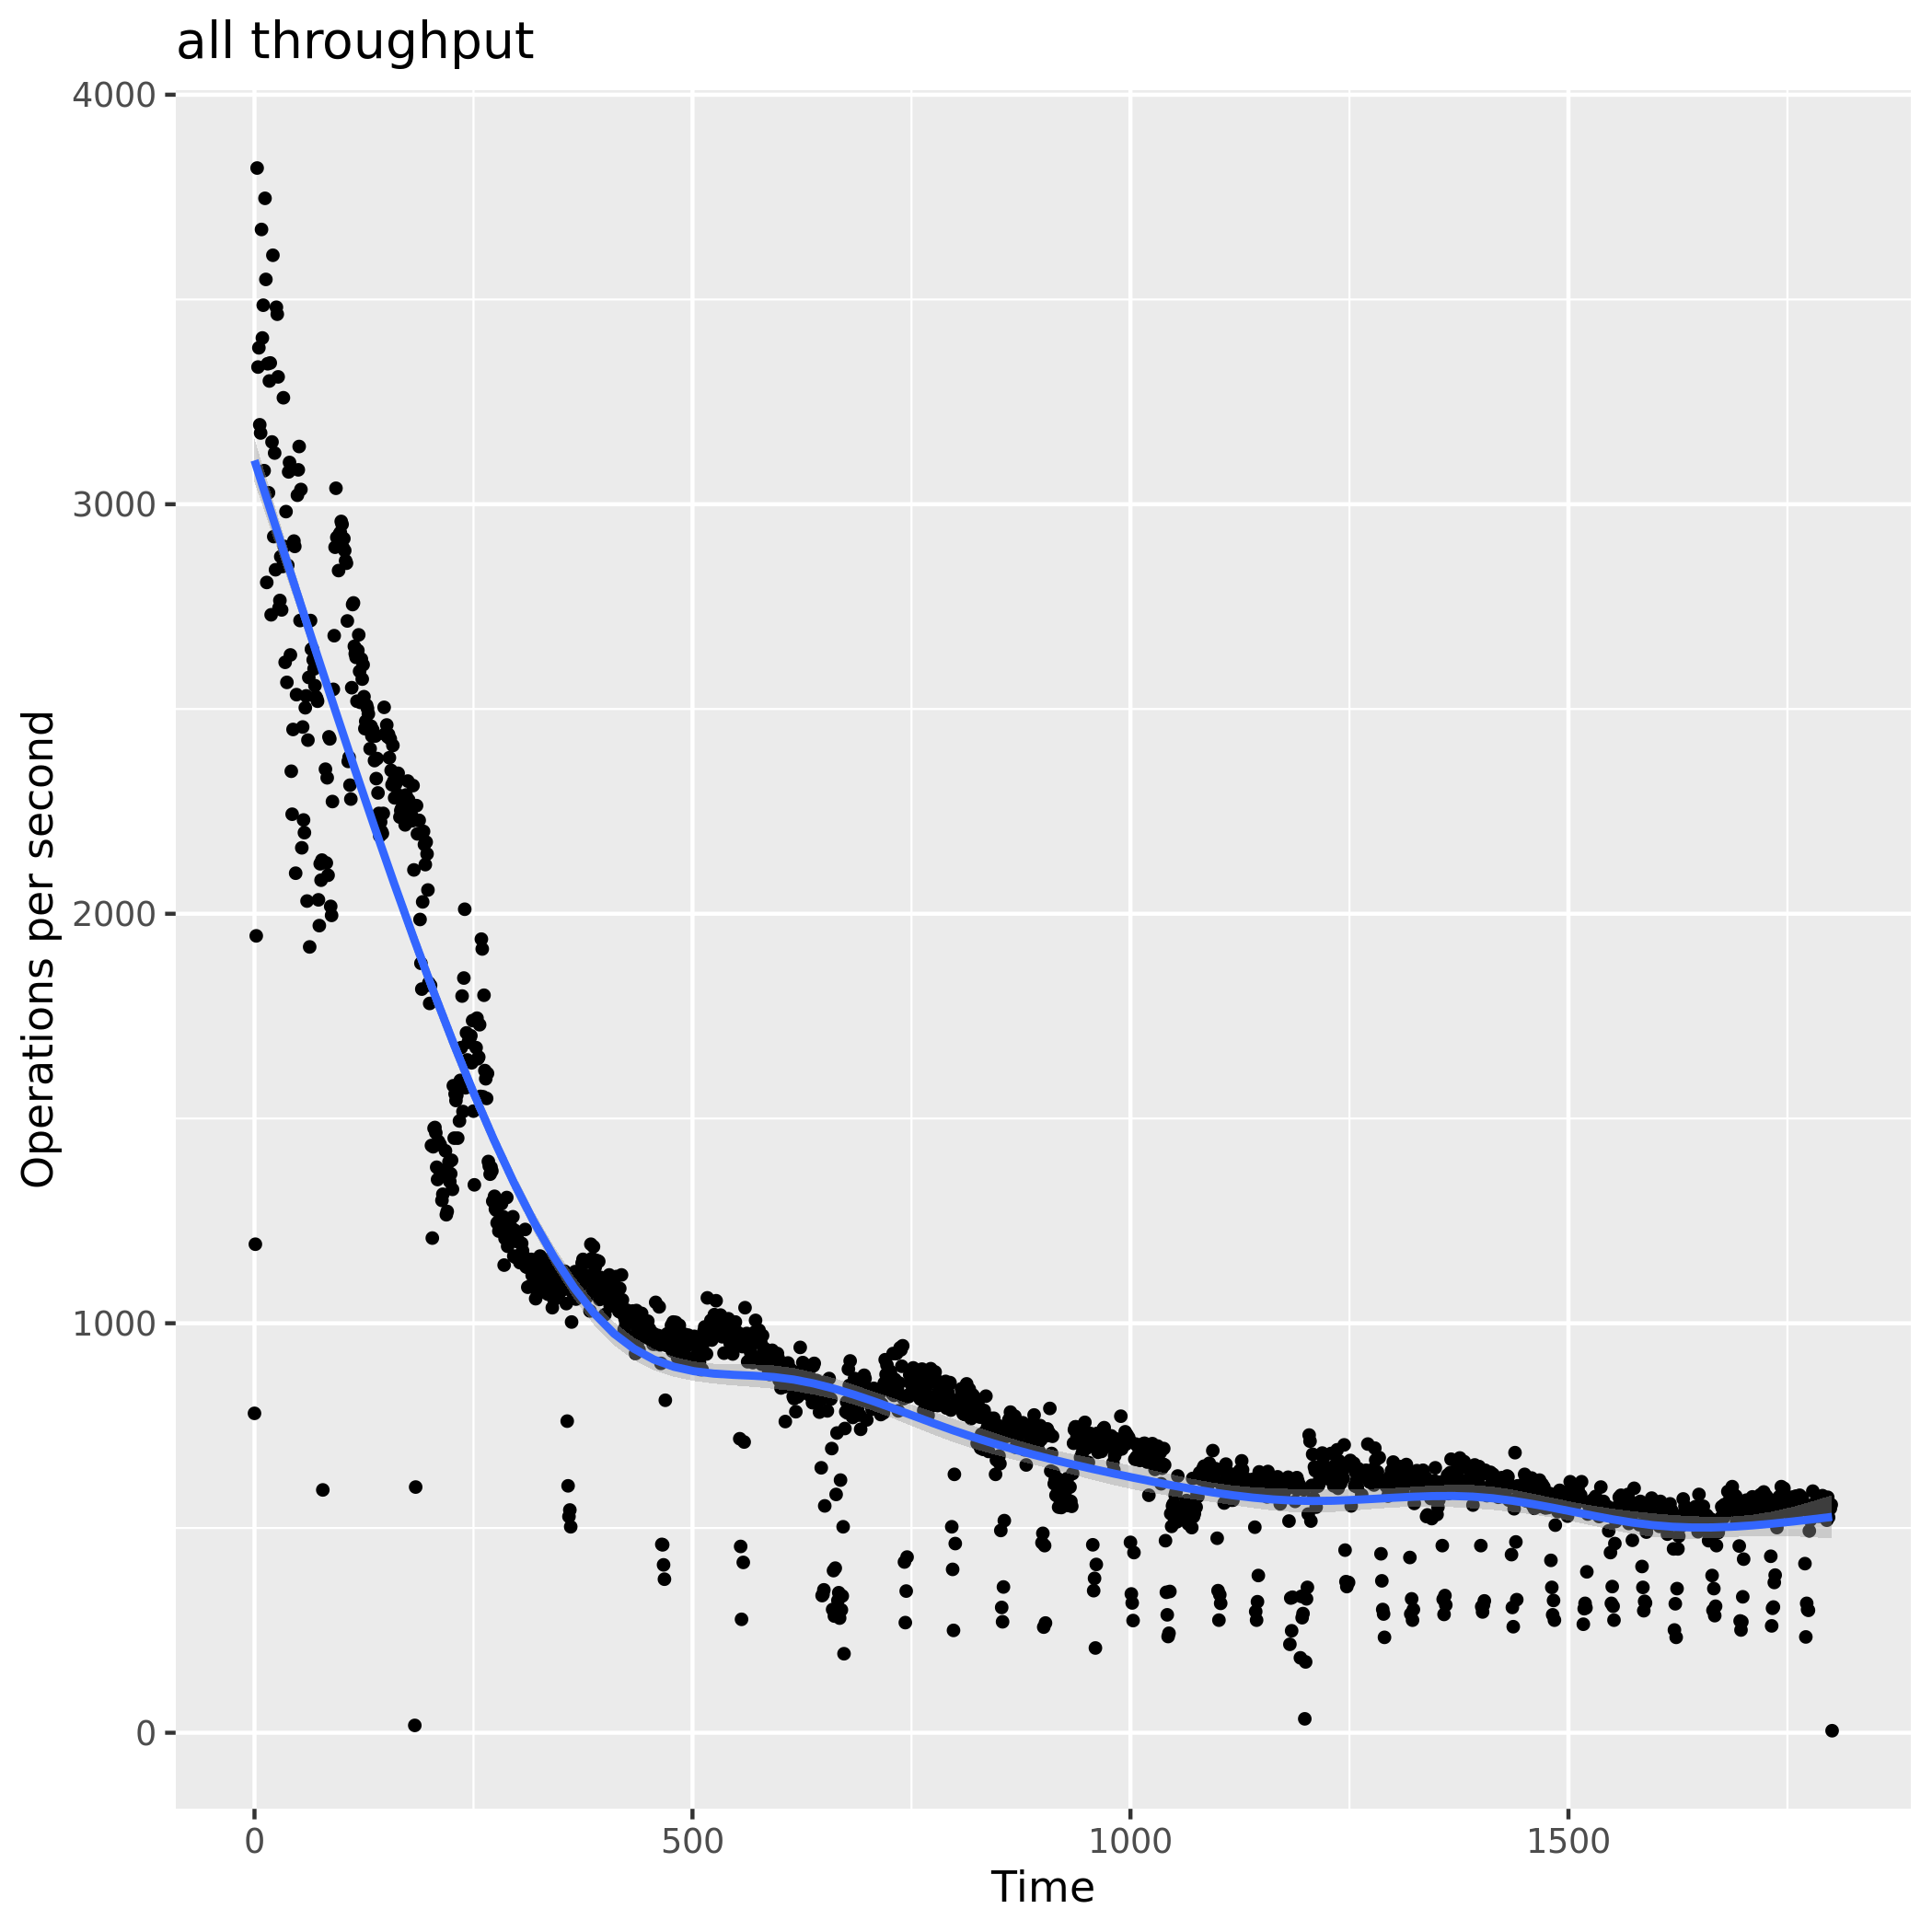
\includegraphics[width=0.5\textwidth]{ConsistentHashing_C1_write_heavy_throughput}
\caption[Throughput Anomaly]{Throughput Anomaly. The throughput shows a steep linear decrease before changing to a shallower linear decrease.}
\label{fig:throughput_anomaly}
\end{figure}

\subsubsection{High Throughput During Handoff}
We expected the benchmark to show a lower throughput and higher latency during the handoffs after a cluster change in the dynamic configuration.
However, as \cref{fig:handoff_anomaly} shows, shortly after the cluster changes at 600s and 1200s the throughput rises to rates much higher than before the change and the latency goes to 0.
This can be explained in one part by rclref vnodes are not handling requests during the handoff and just acknowledging it, and in another part that rclref uses one ets table per vnode and as a consequence of the cluster change there are new vnodes with empty ets tables.
\begin{figure}
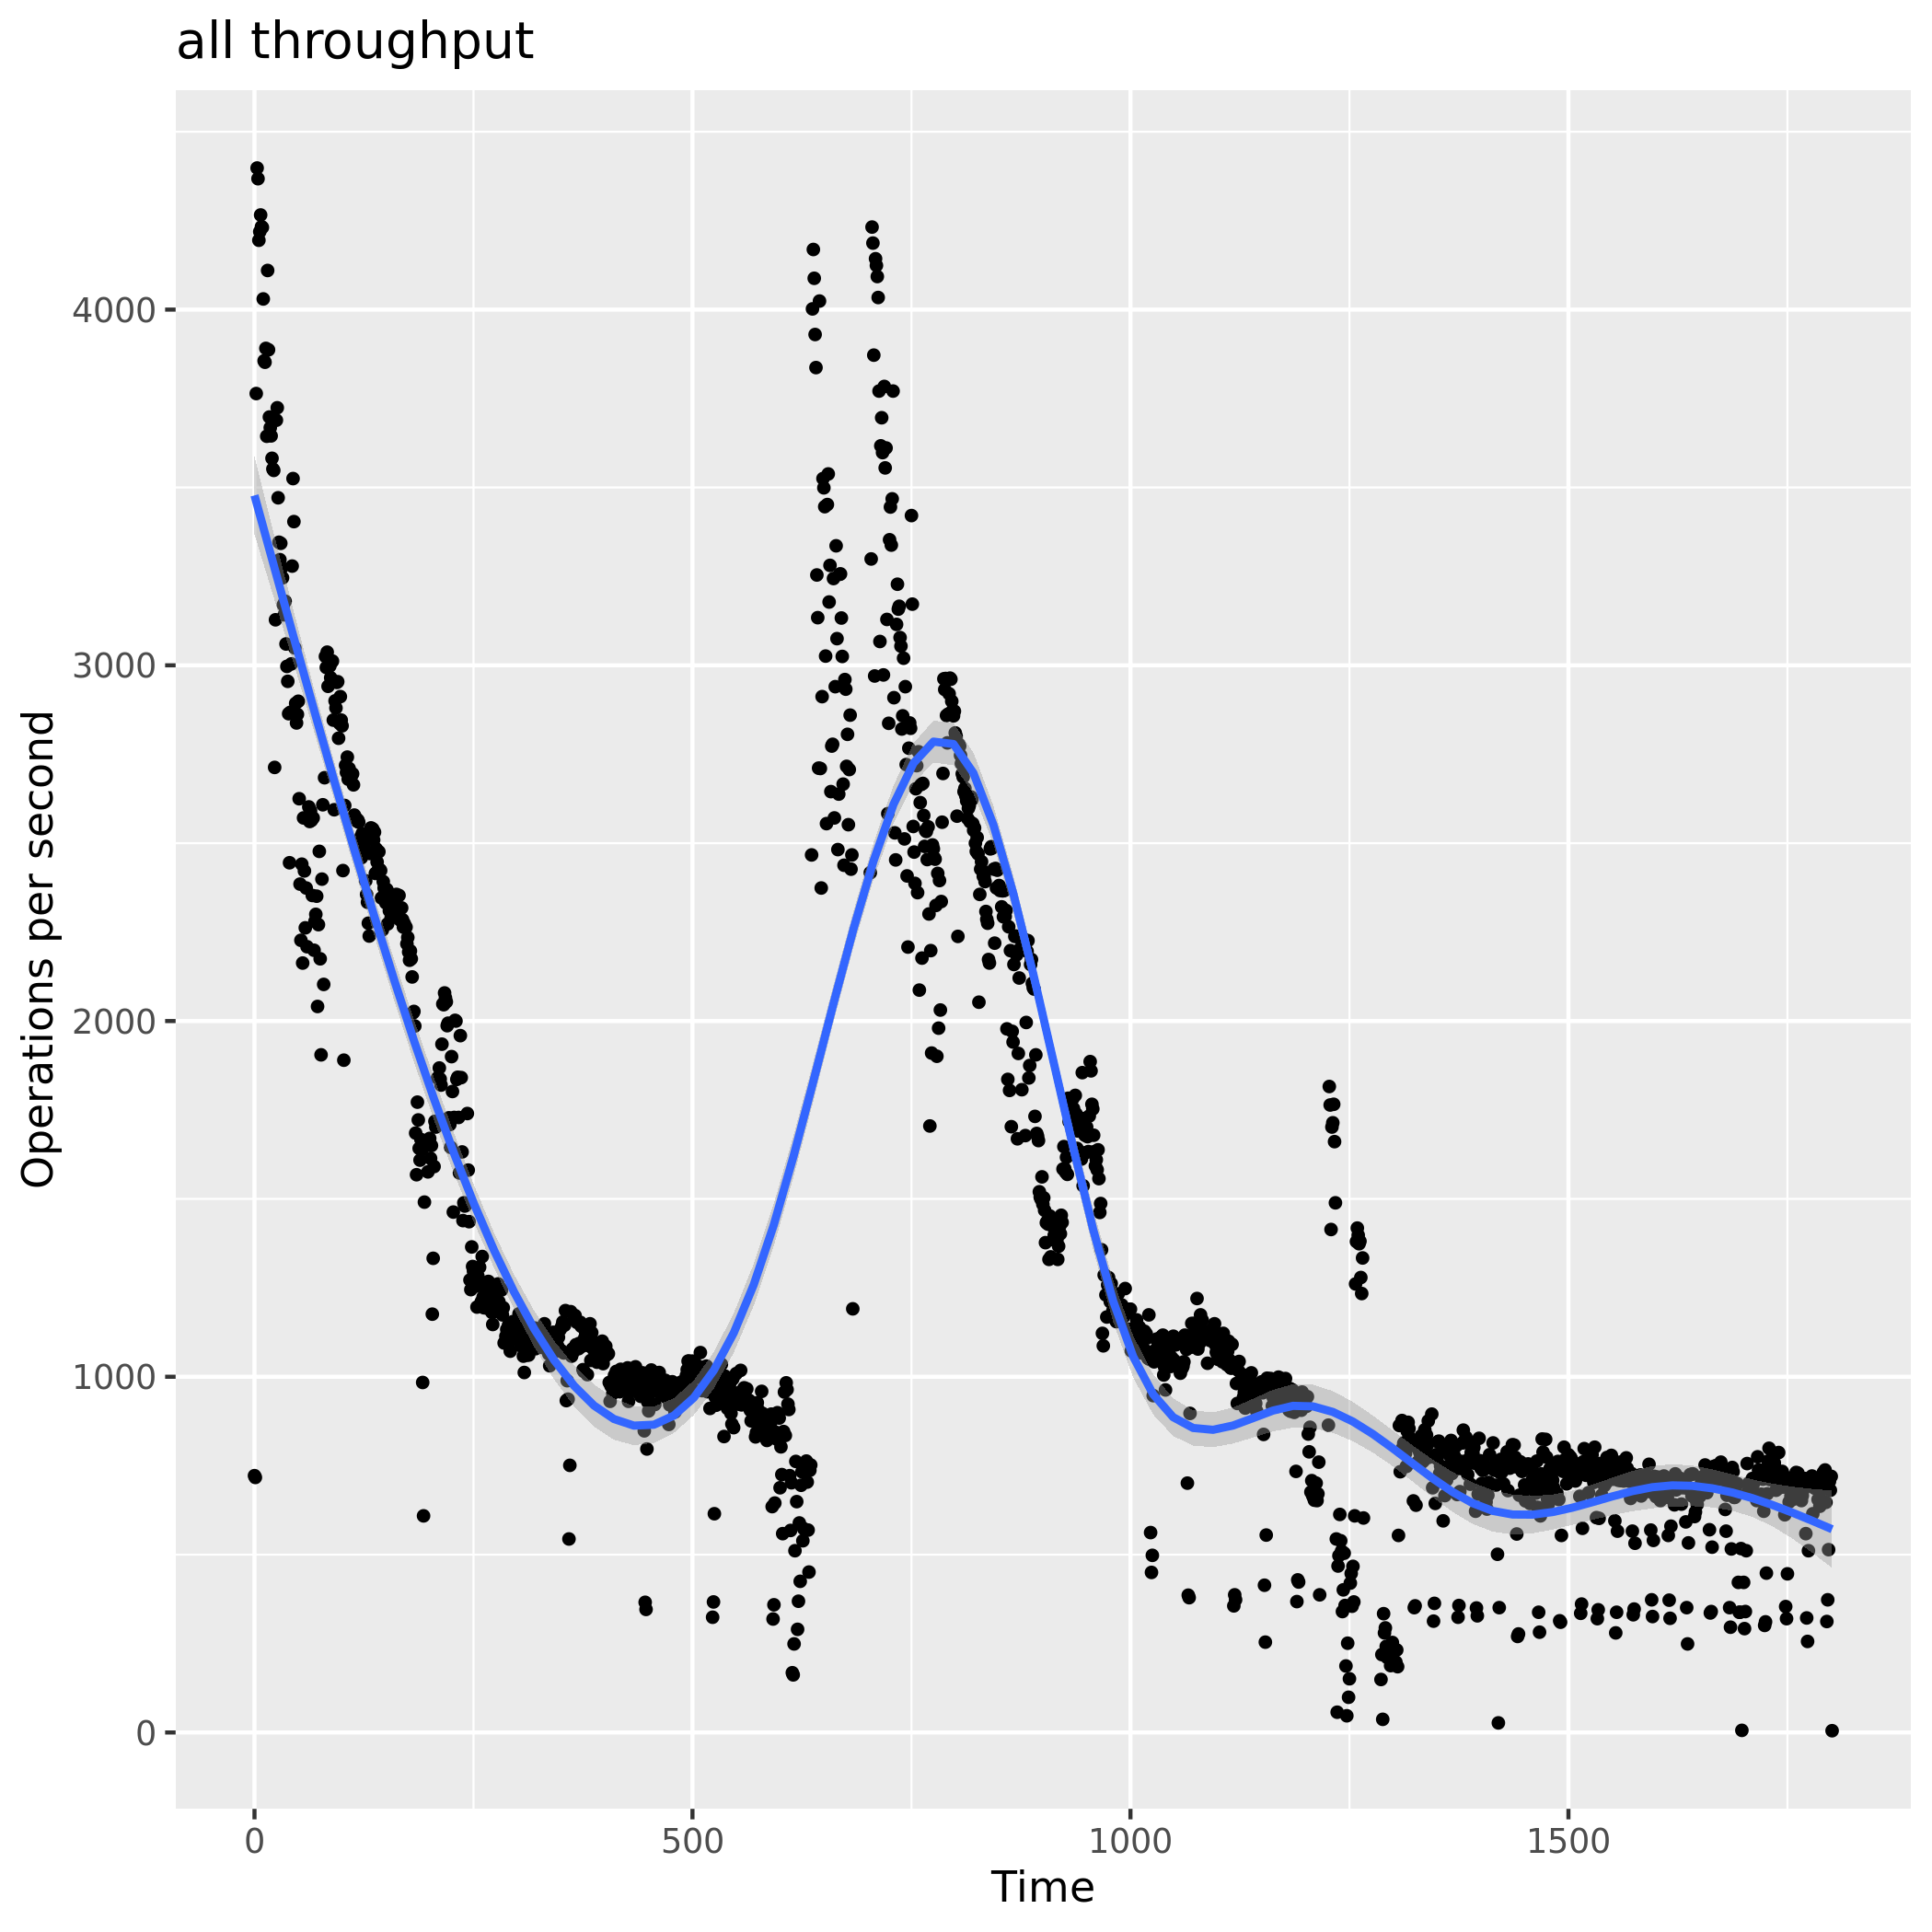
\includegraphics[width=0.5\textwidth]{ConsistentHashing_dynamic_write_heavy_throughput}
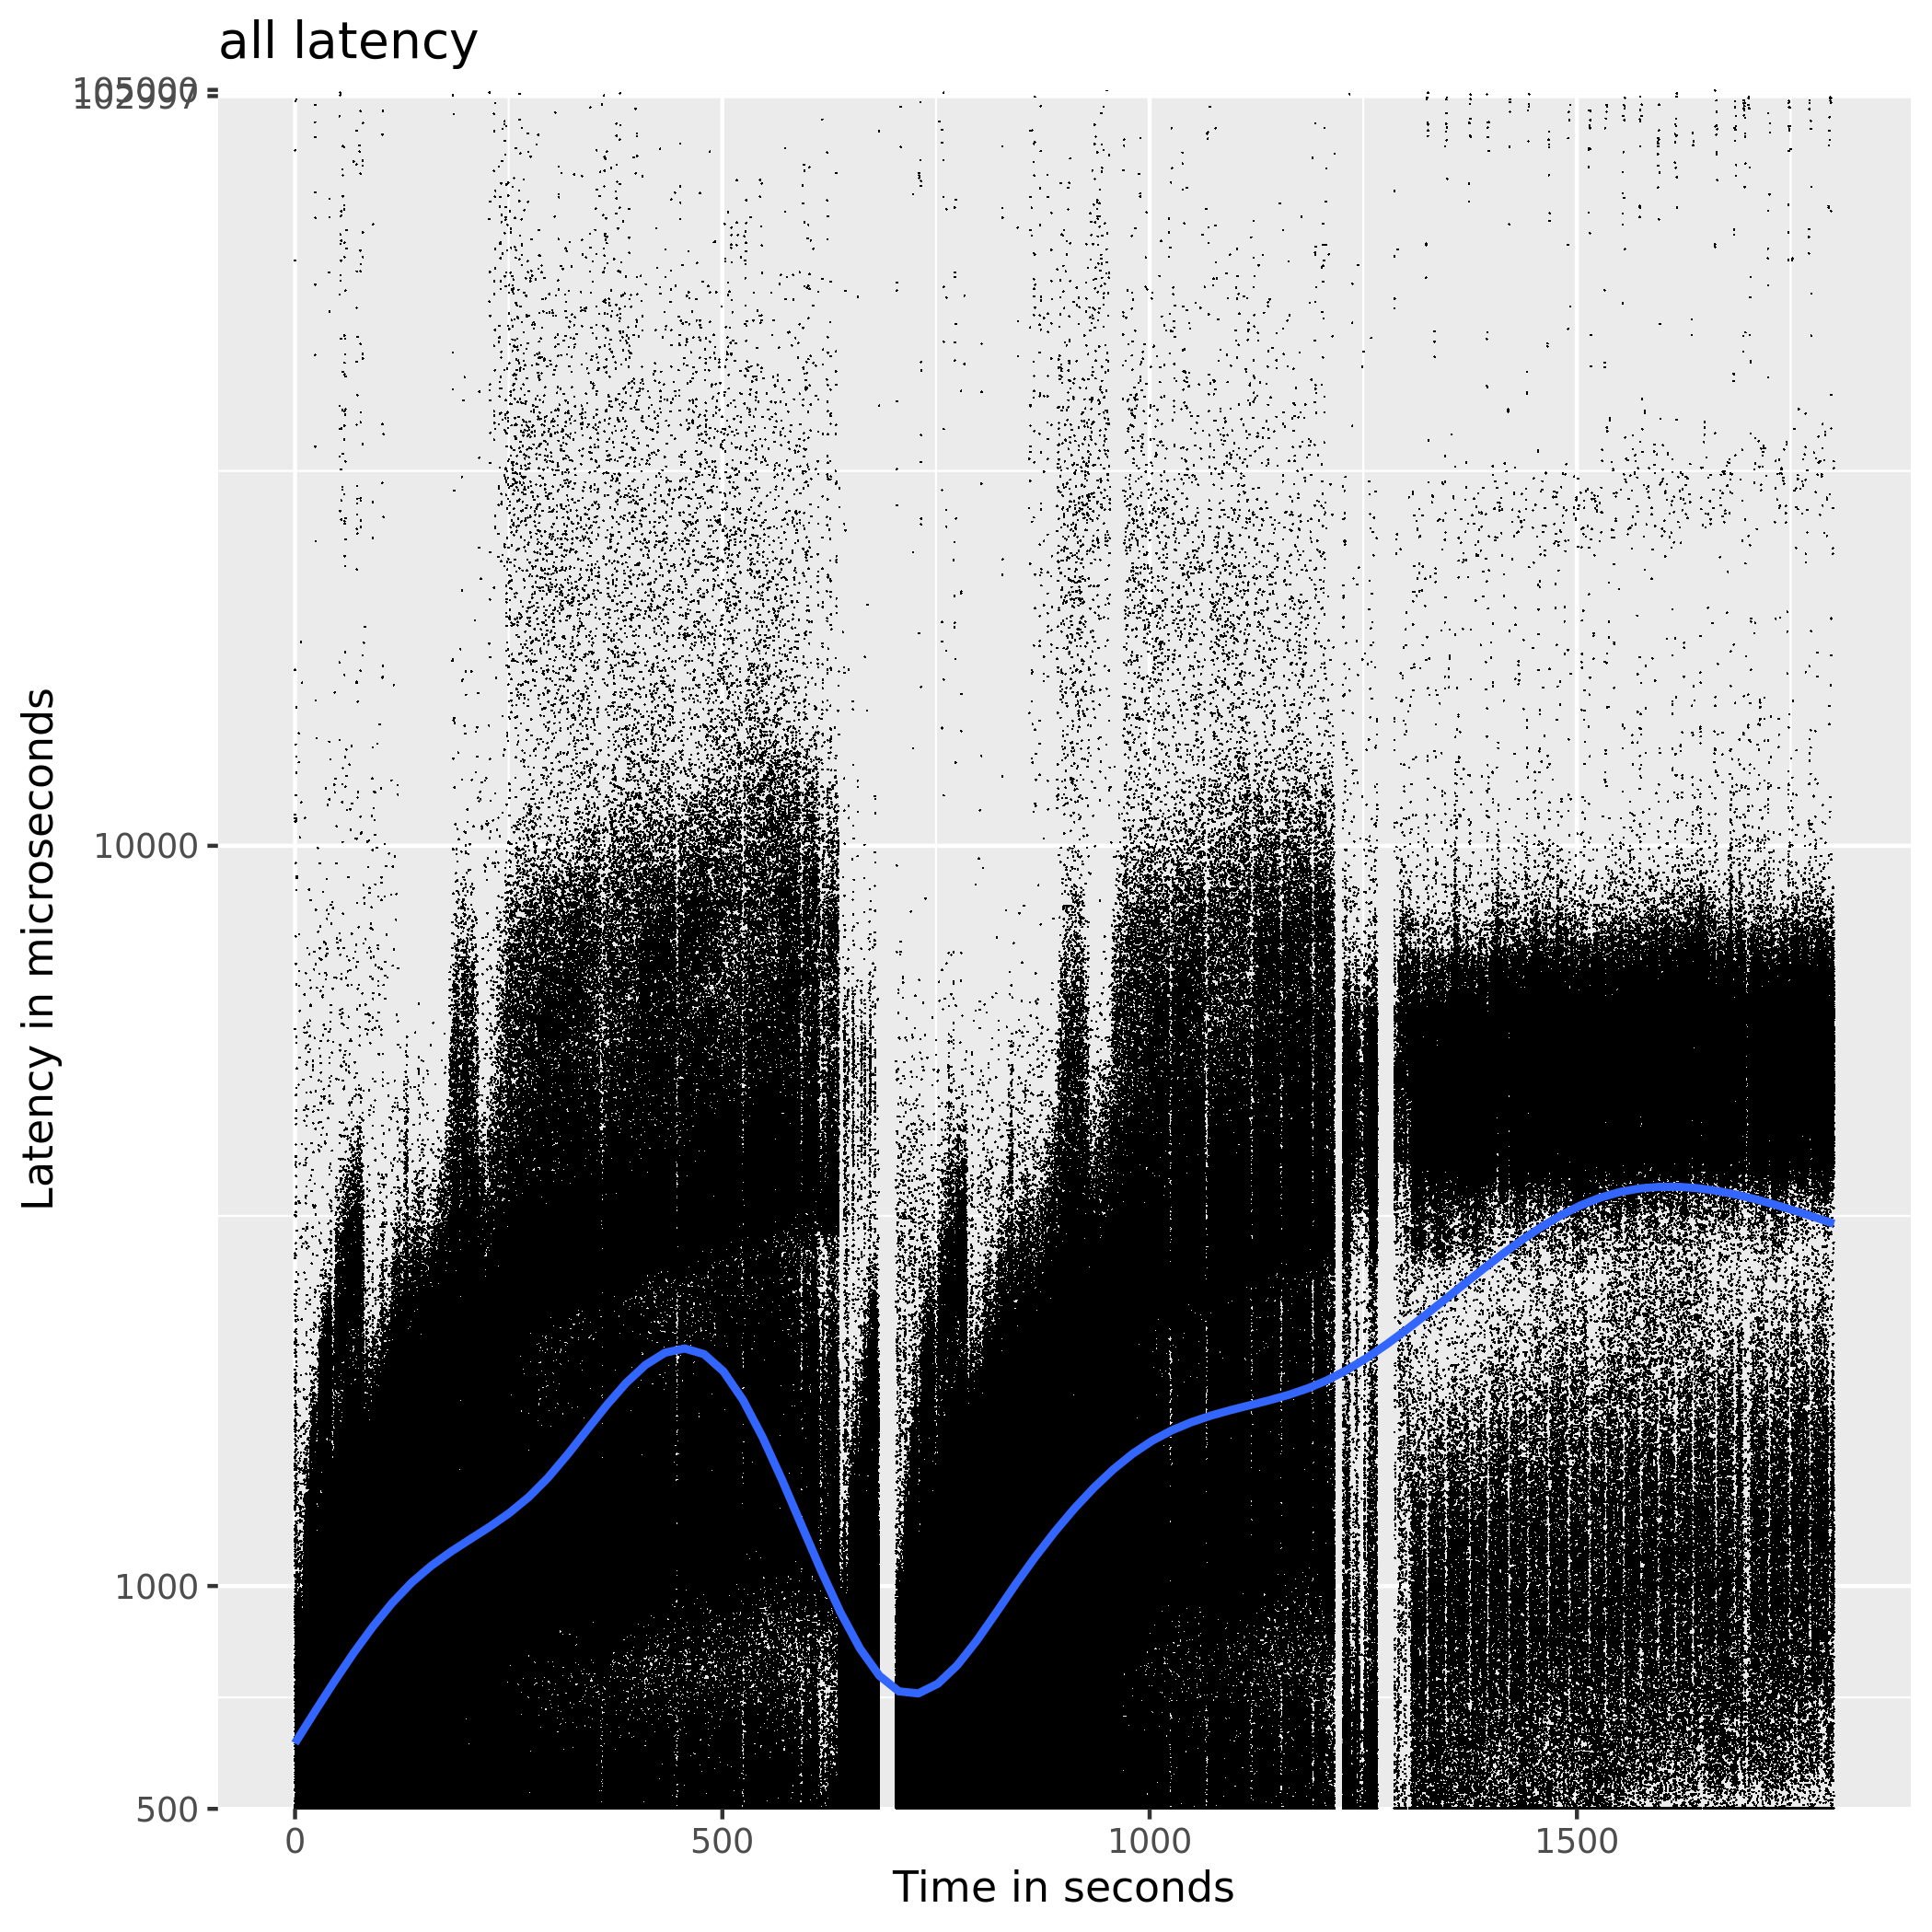
\includegraphics[width=0.5\textwidth]{ConsistentHashing_dynamic_write_heavy_latency}
\caption[Handoff Anomaly]{Handoff Anomaly. Instead of a low throughput and high latency after a cluster change the system has a high throughput and low latency.}
\label{fig:handoff_anomaly}
\end{figure}

\subsubsection{Optimal Load Balance in C0 with Random Slicing}
In configuration C0 with just three nodes \ac{RS} achieves a perfect load balance with the exact same number of keys stored on each node with any of the \acp{RPS}.
This can easily be explained by the nature of \ac{RS}.
Since the three nodes are the initial configuration, \ac{RS} produces a ring with exactly three sections, one for each node.
With $n=3$ set in the configuration each key is therefore replicated on three sections, which leads to each node storing each key and therefore owning the same number of keys.
As for configurations with Consistent Hashing the ring size is set to 64 the sections cannot be perfectly assigned to three nodes and therefore this configuration does not achieve a perfect load balance.

\subsection{Consistent Hashing}
With Consistent Hashing there is no significant difference between read-heavy and write-heavy workloads.
A visualization of runs in C0 and C2 is shown in \cref{fig:throughput_consistent_hashing}
There is a clear trend of lower throughput with a higher number of nodes.
In configuration C0 with three nodes the average throughput starts at about 3500 operations per second, steeply decreases to 1000 operations per second at about 450s and from there slowly decreases to 500 operations per second.
In configuration C1 with four nodes there is no clear difference to C0.
However, in configuration C2 with seven nodes the average throughput starts at about 750 operations per second, there is no steep decrease, and it slowly decreases to 450 operations per second.
One can see, that while starting out at a way lower rate the throughput ends up at a closer rate between the configurations.
\begin{figure}
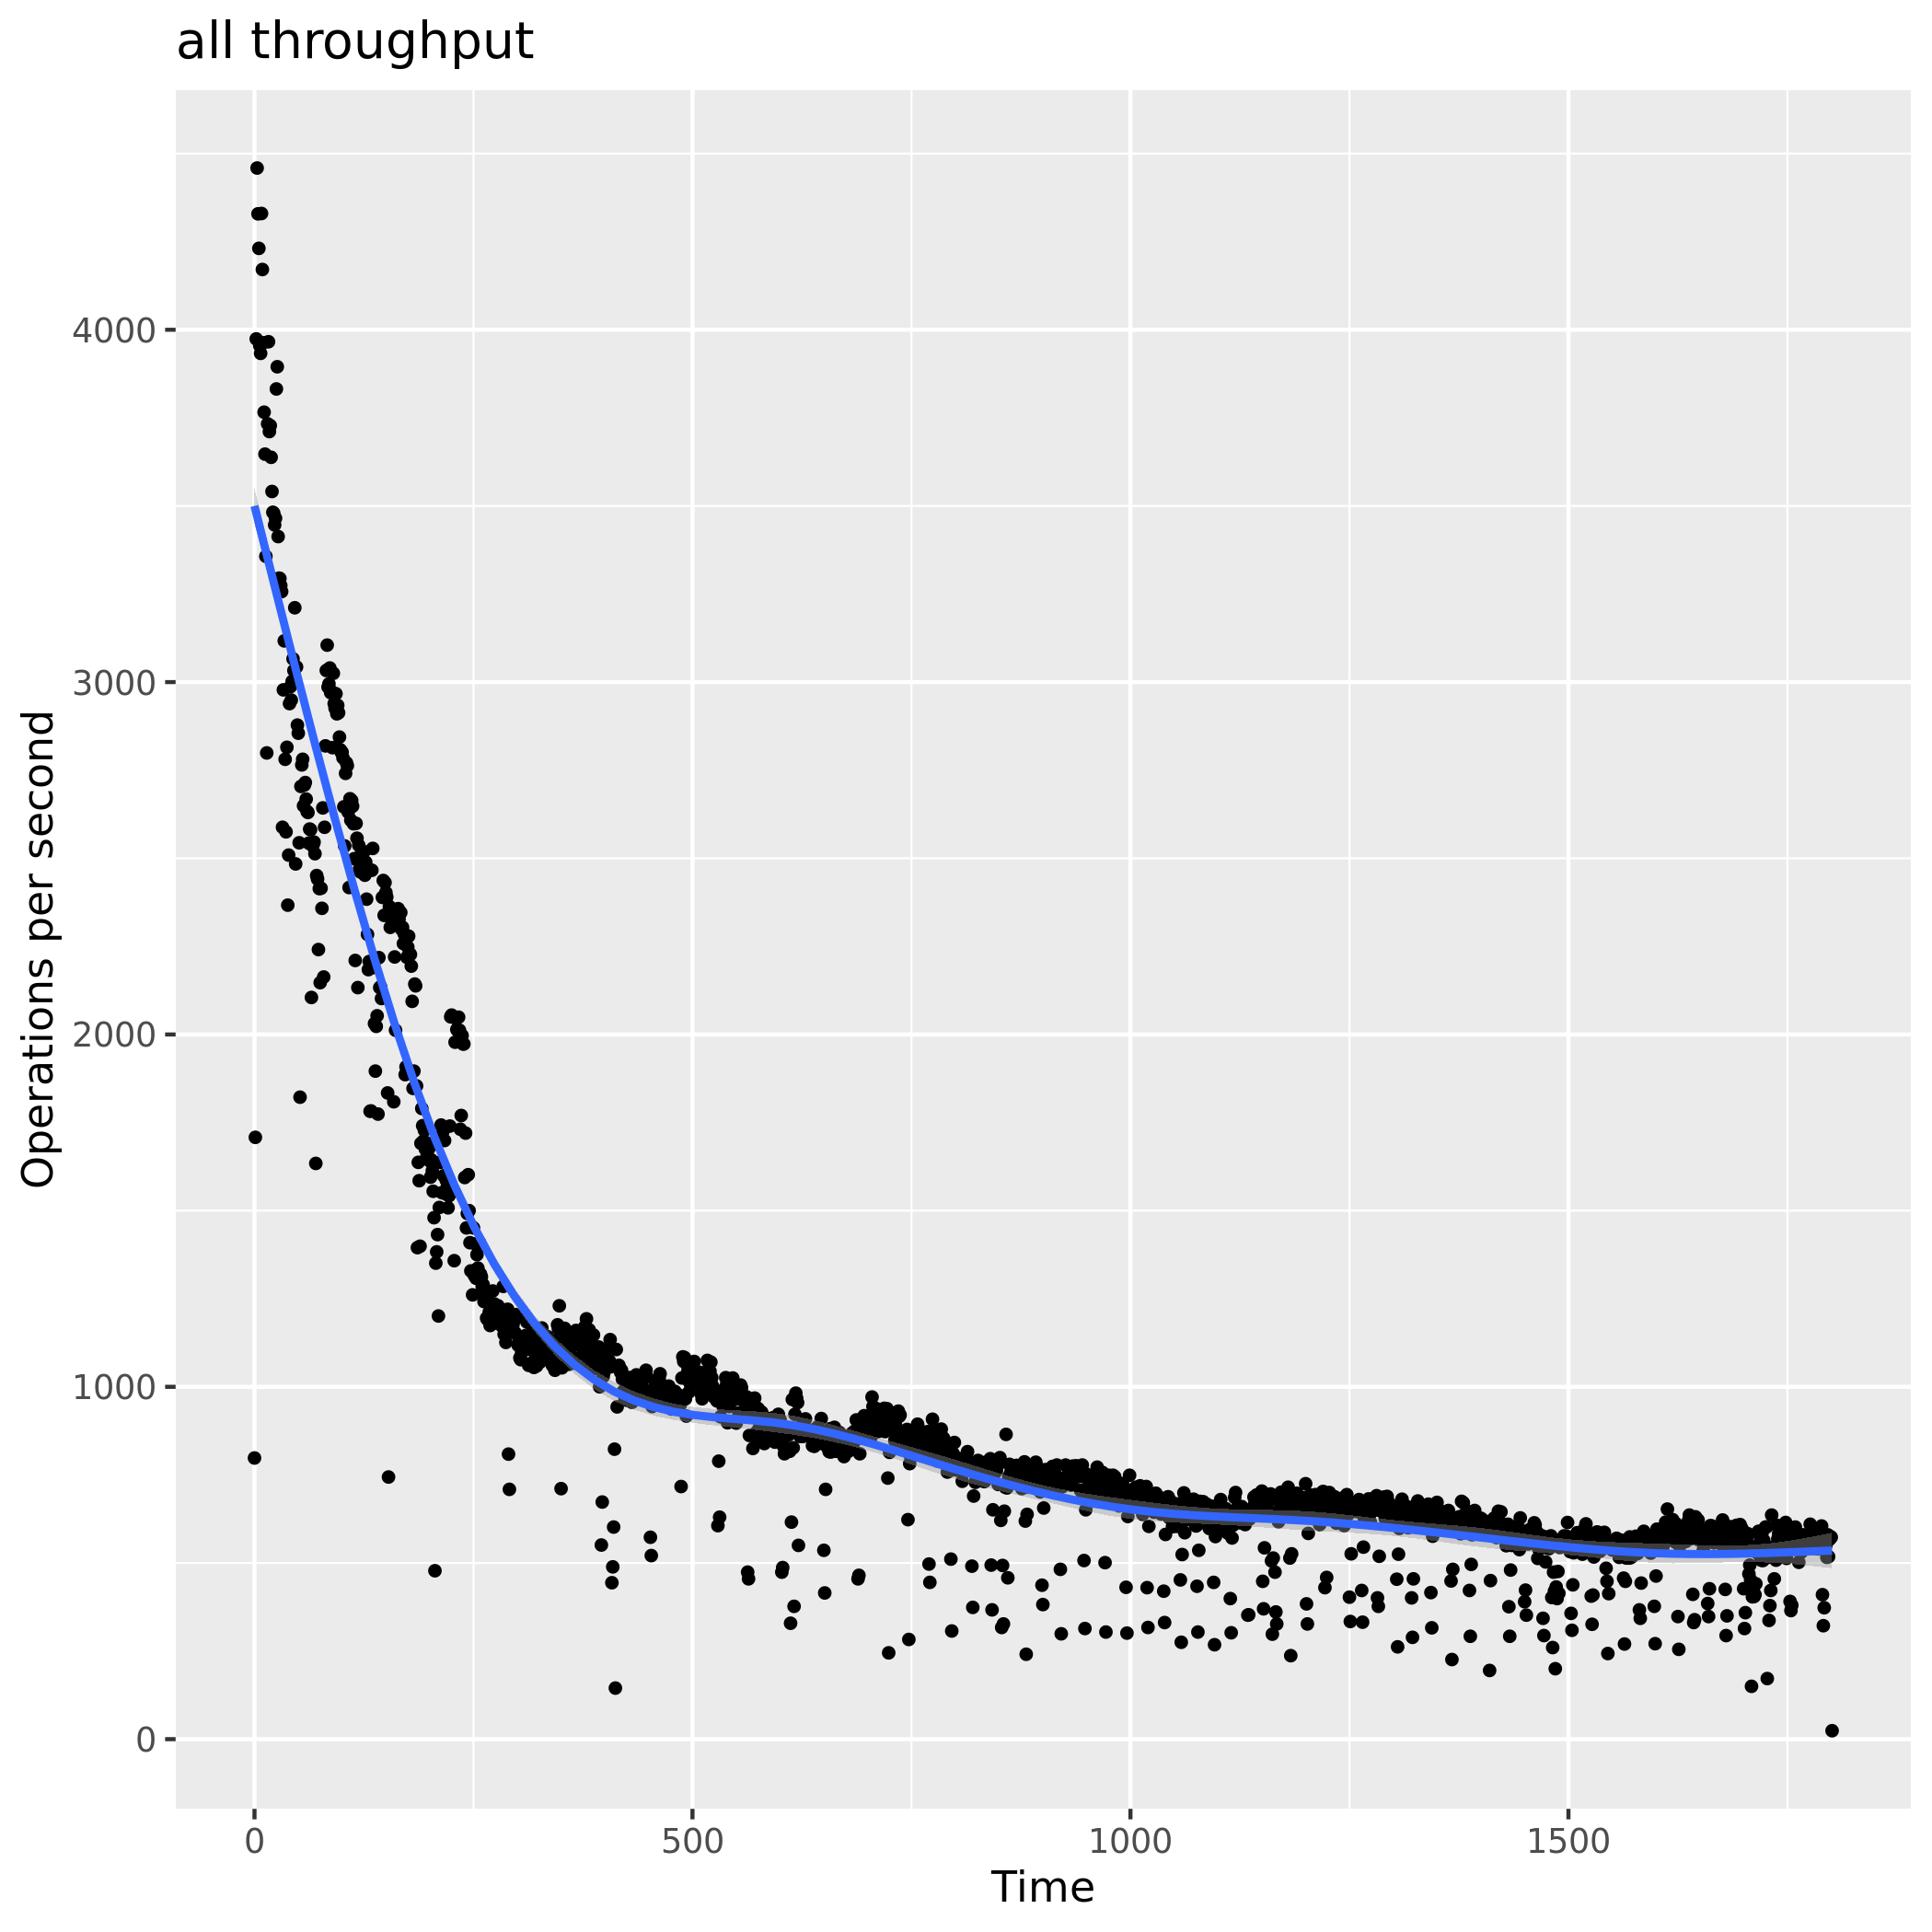
\includegraphics[width=0.5\textwidth]{ConsistentHashing_C0_write_heavy_throughput}
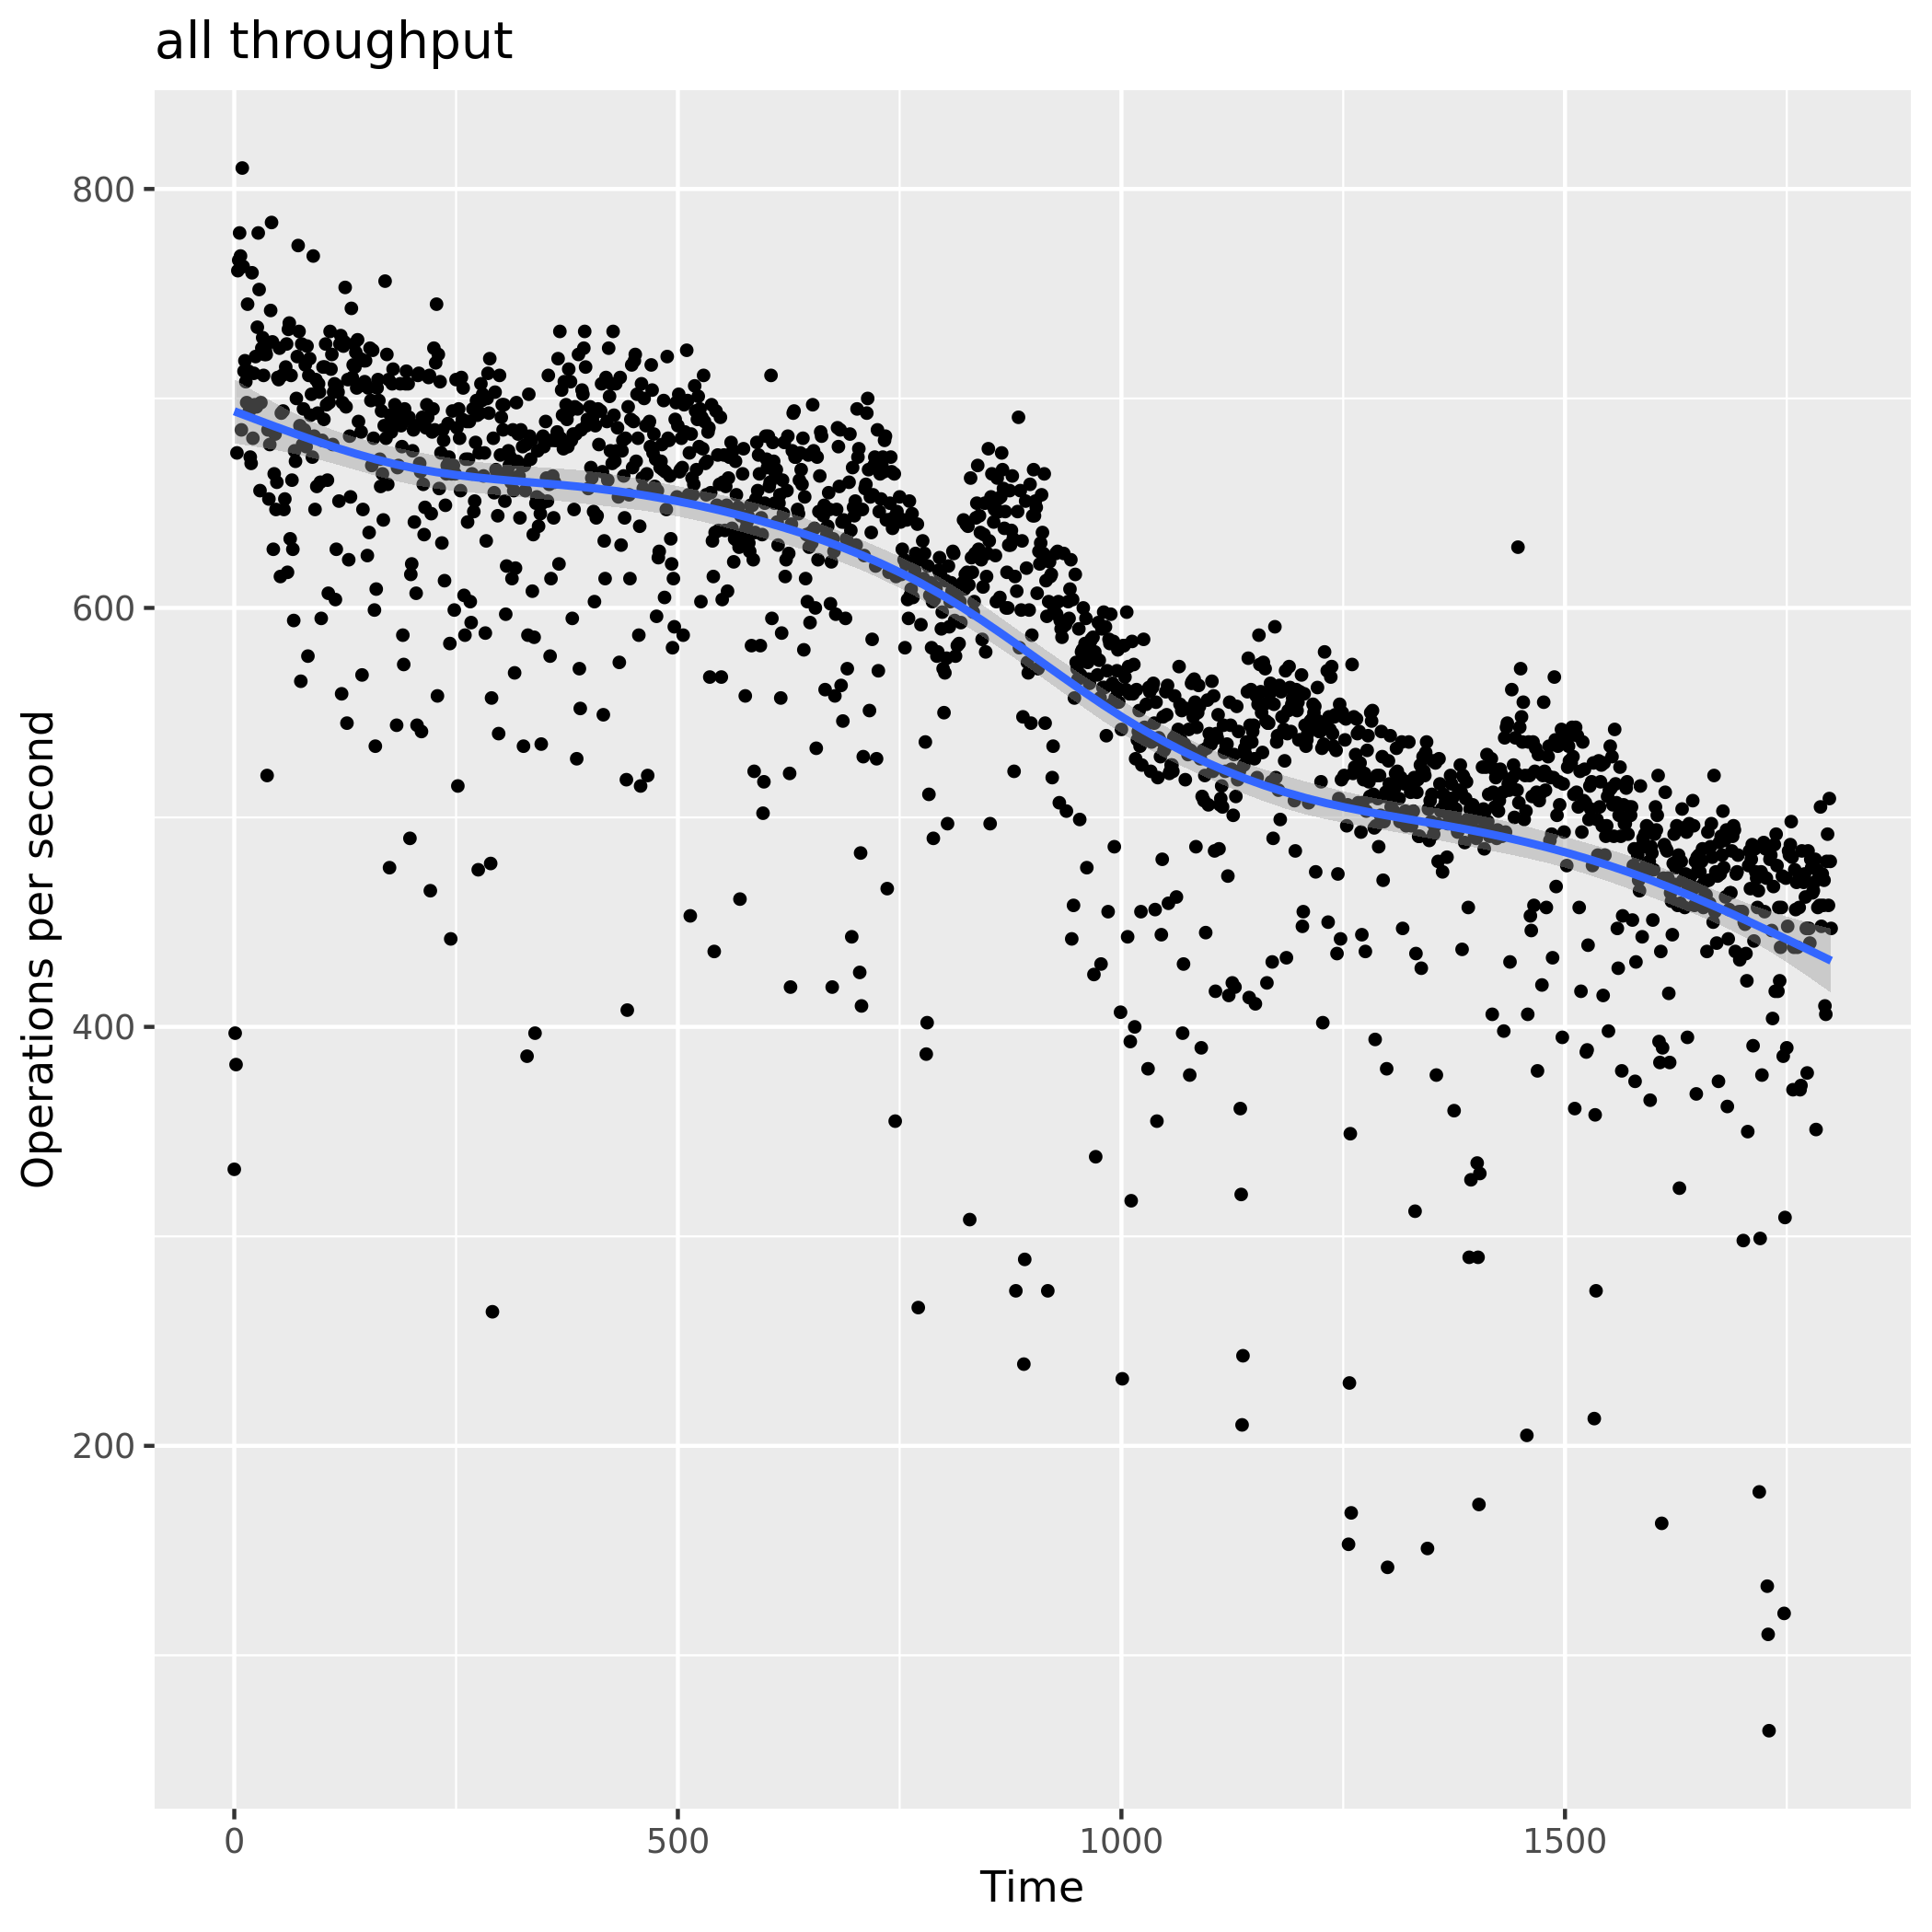
\includegraphics[width=0.5\textwidth]{ConsistentHashing_C2_write_heavy_throughput}
\caption[Consistent Hashing Throughput Comparison]{Consistent Hashing Throughput Comparison. Showing the throughput for Consistent Hashing in C0 and C2 with write-heavy workload.}
\label{fig:throughput_consistent_hashing}
\end{figure}

For the dynamic benchmark runs there are significant differences between read-heavy and write-heavy workload.
Ignoring the impact of the cluster changes the throughput plot seems to be quite similar as it decreases to 1000 operations per second within 450 seconds and after that decreases to about 600 operations per second.
However, it seems that for the read-heavy workload the change from C0 to C1 does not have a great impact on the throughput or latency while it has a significant impact during the write-heavy workload.
This can be seen both in the throughput and latency plots in \cref{fig:consistent_hashing_dynamic}.
For the change from C1 to C2 at 1200s the impact of the workload seems to be inverse to the ones of the change from C0 to C1.
\begin{figure}
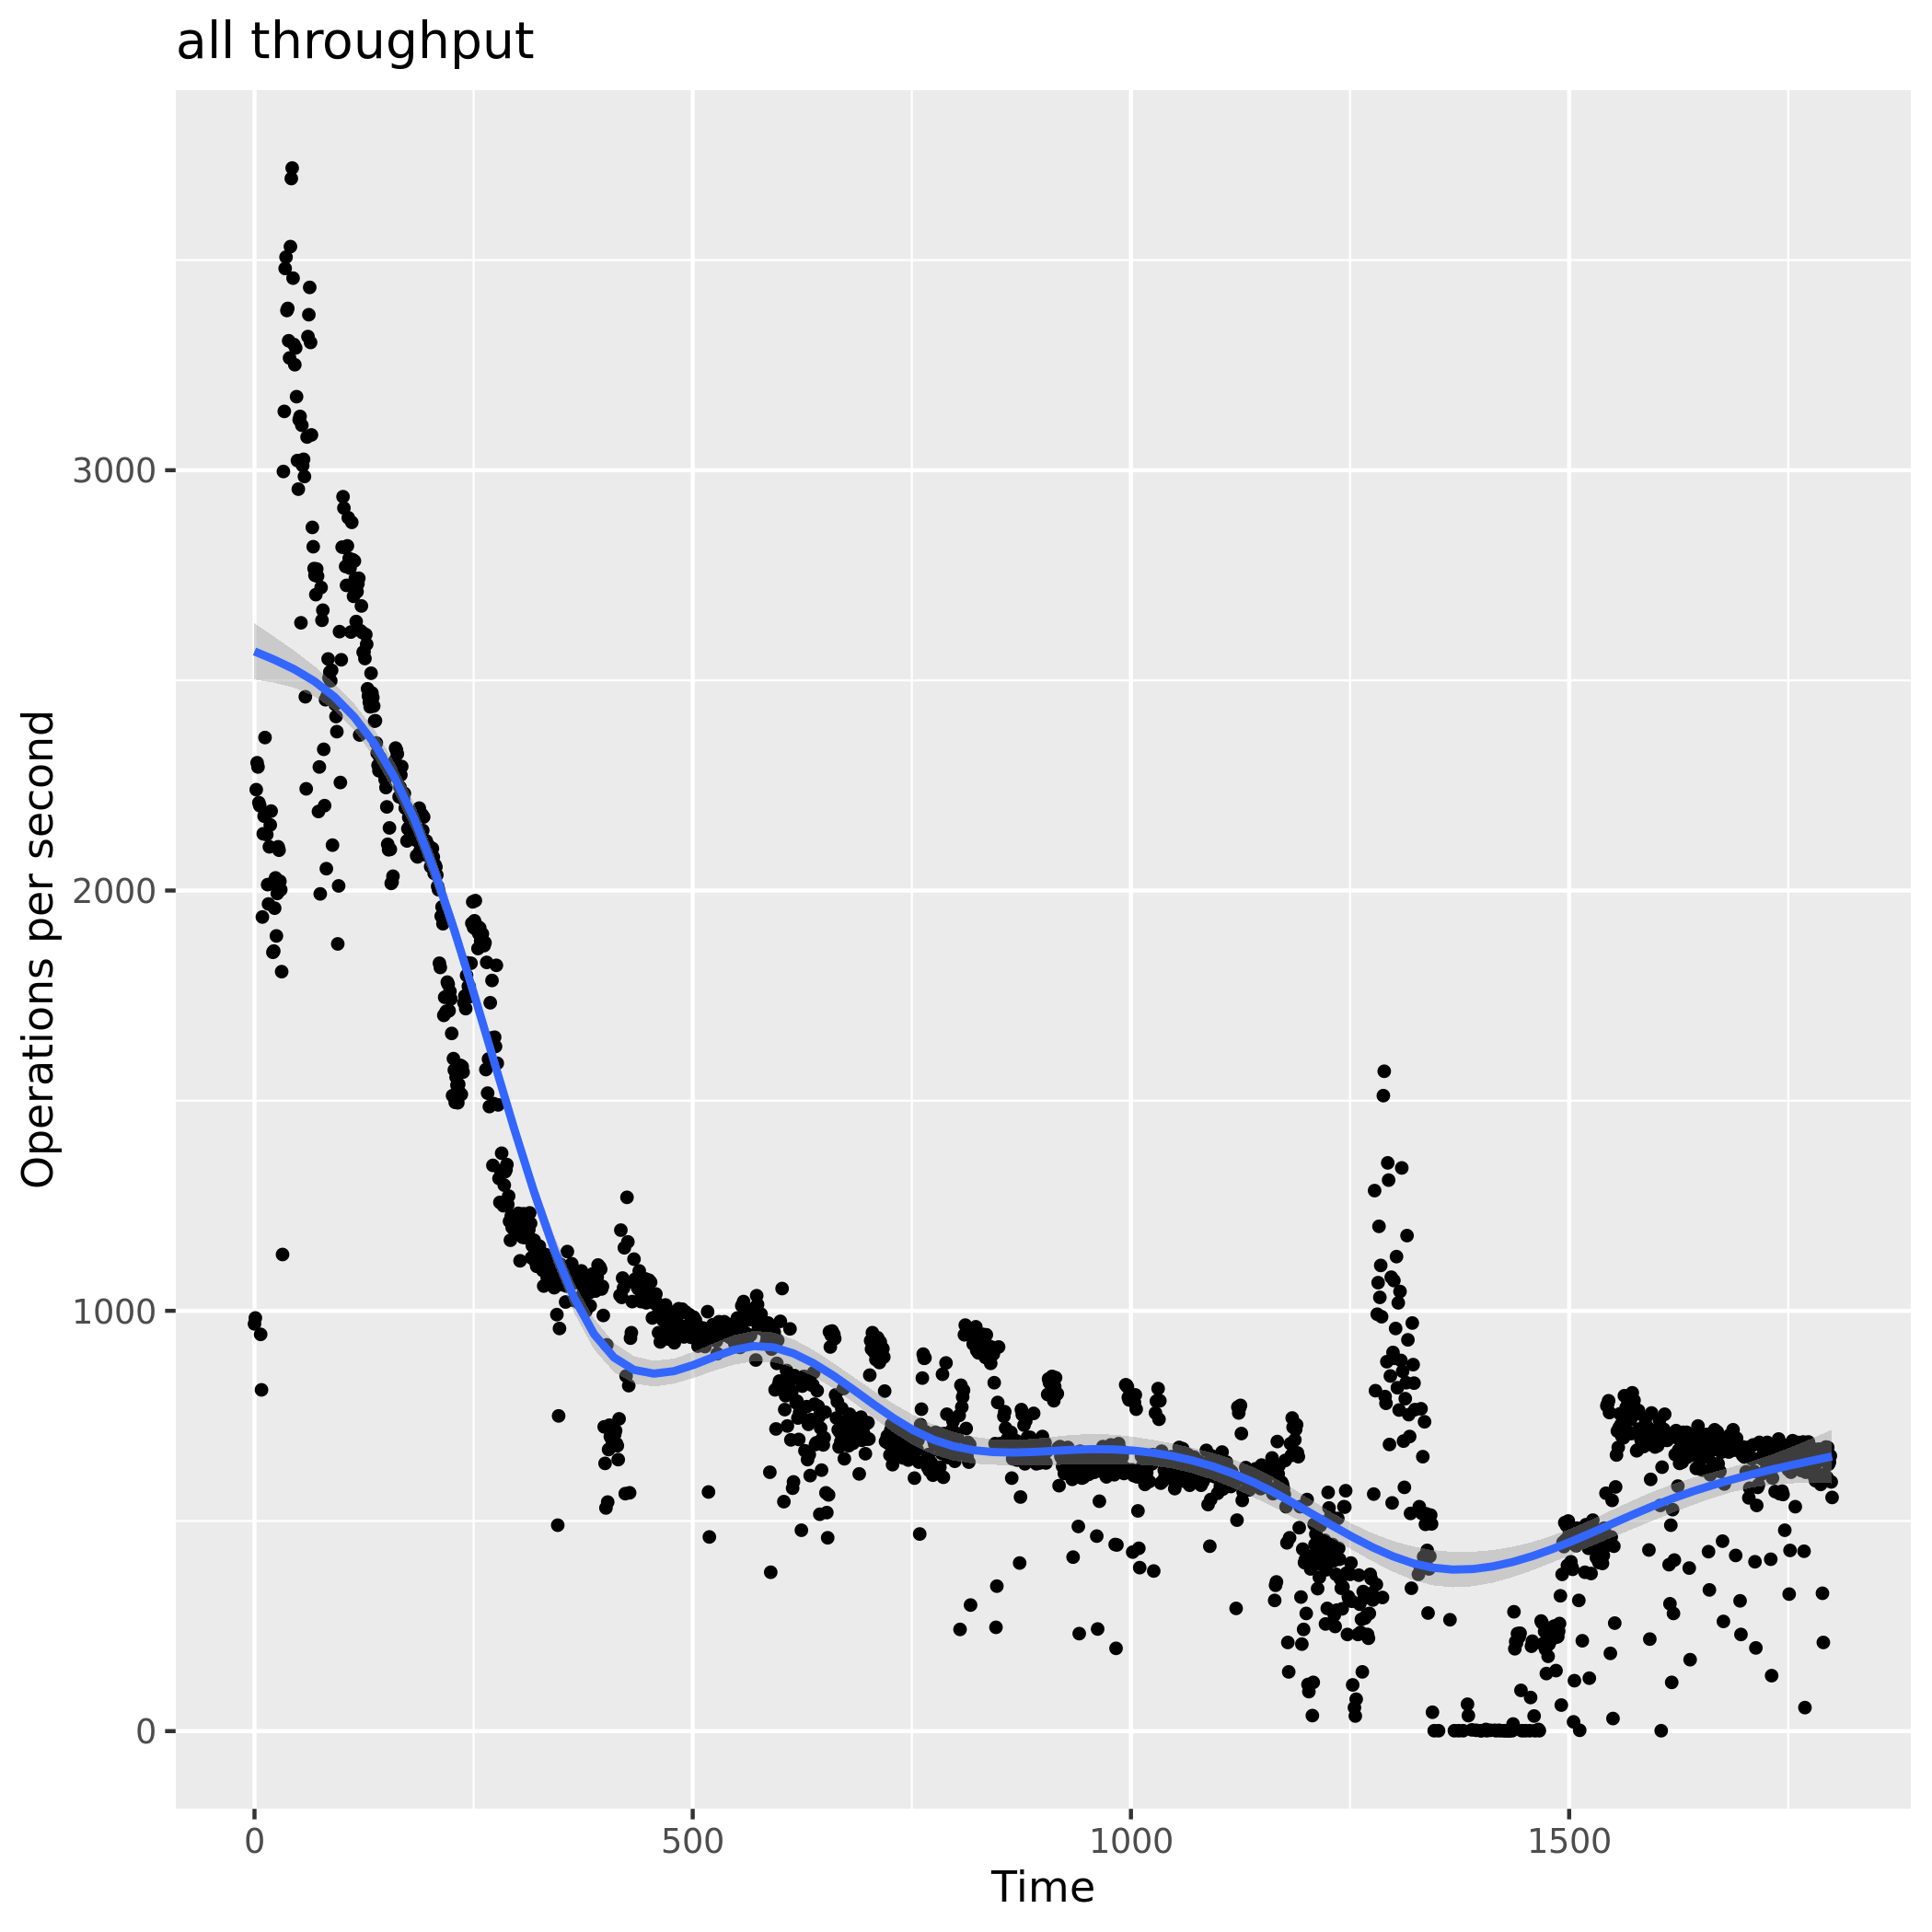
\includegraphics[width=0.5\textwidth]{ConsistentHashing_dynamic_read_heavy_throughput}
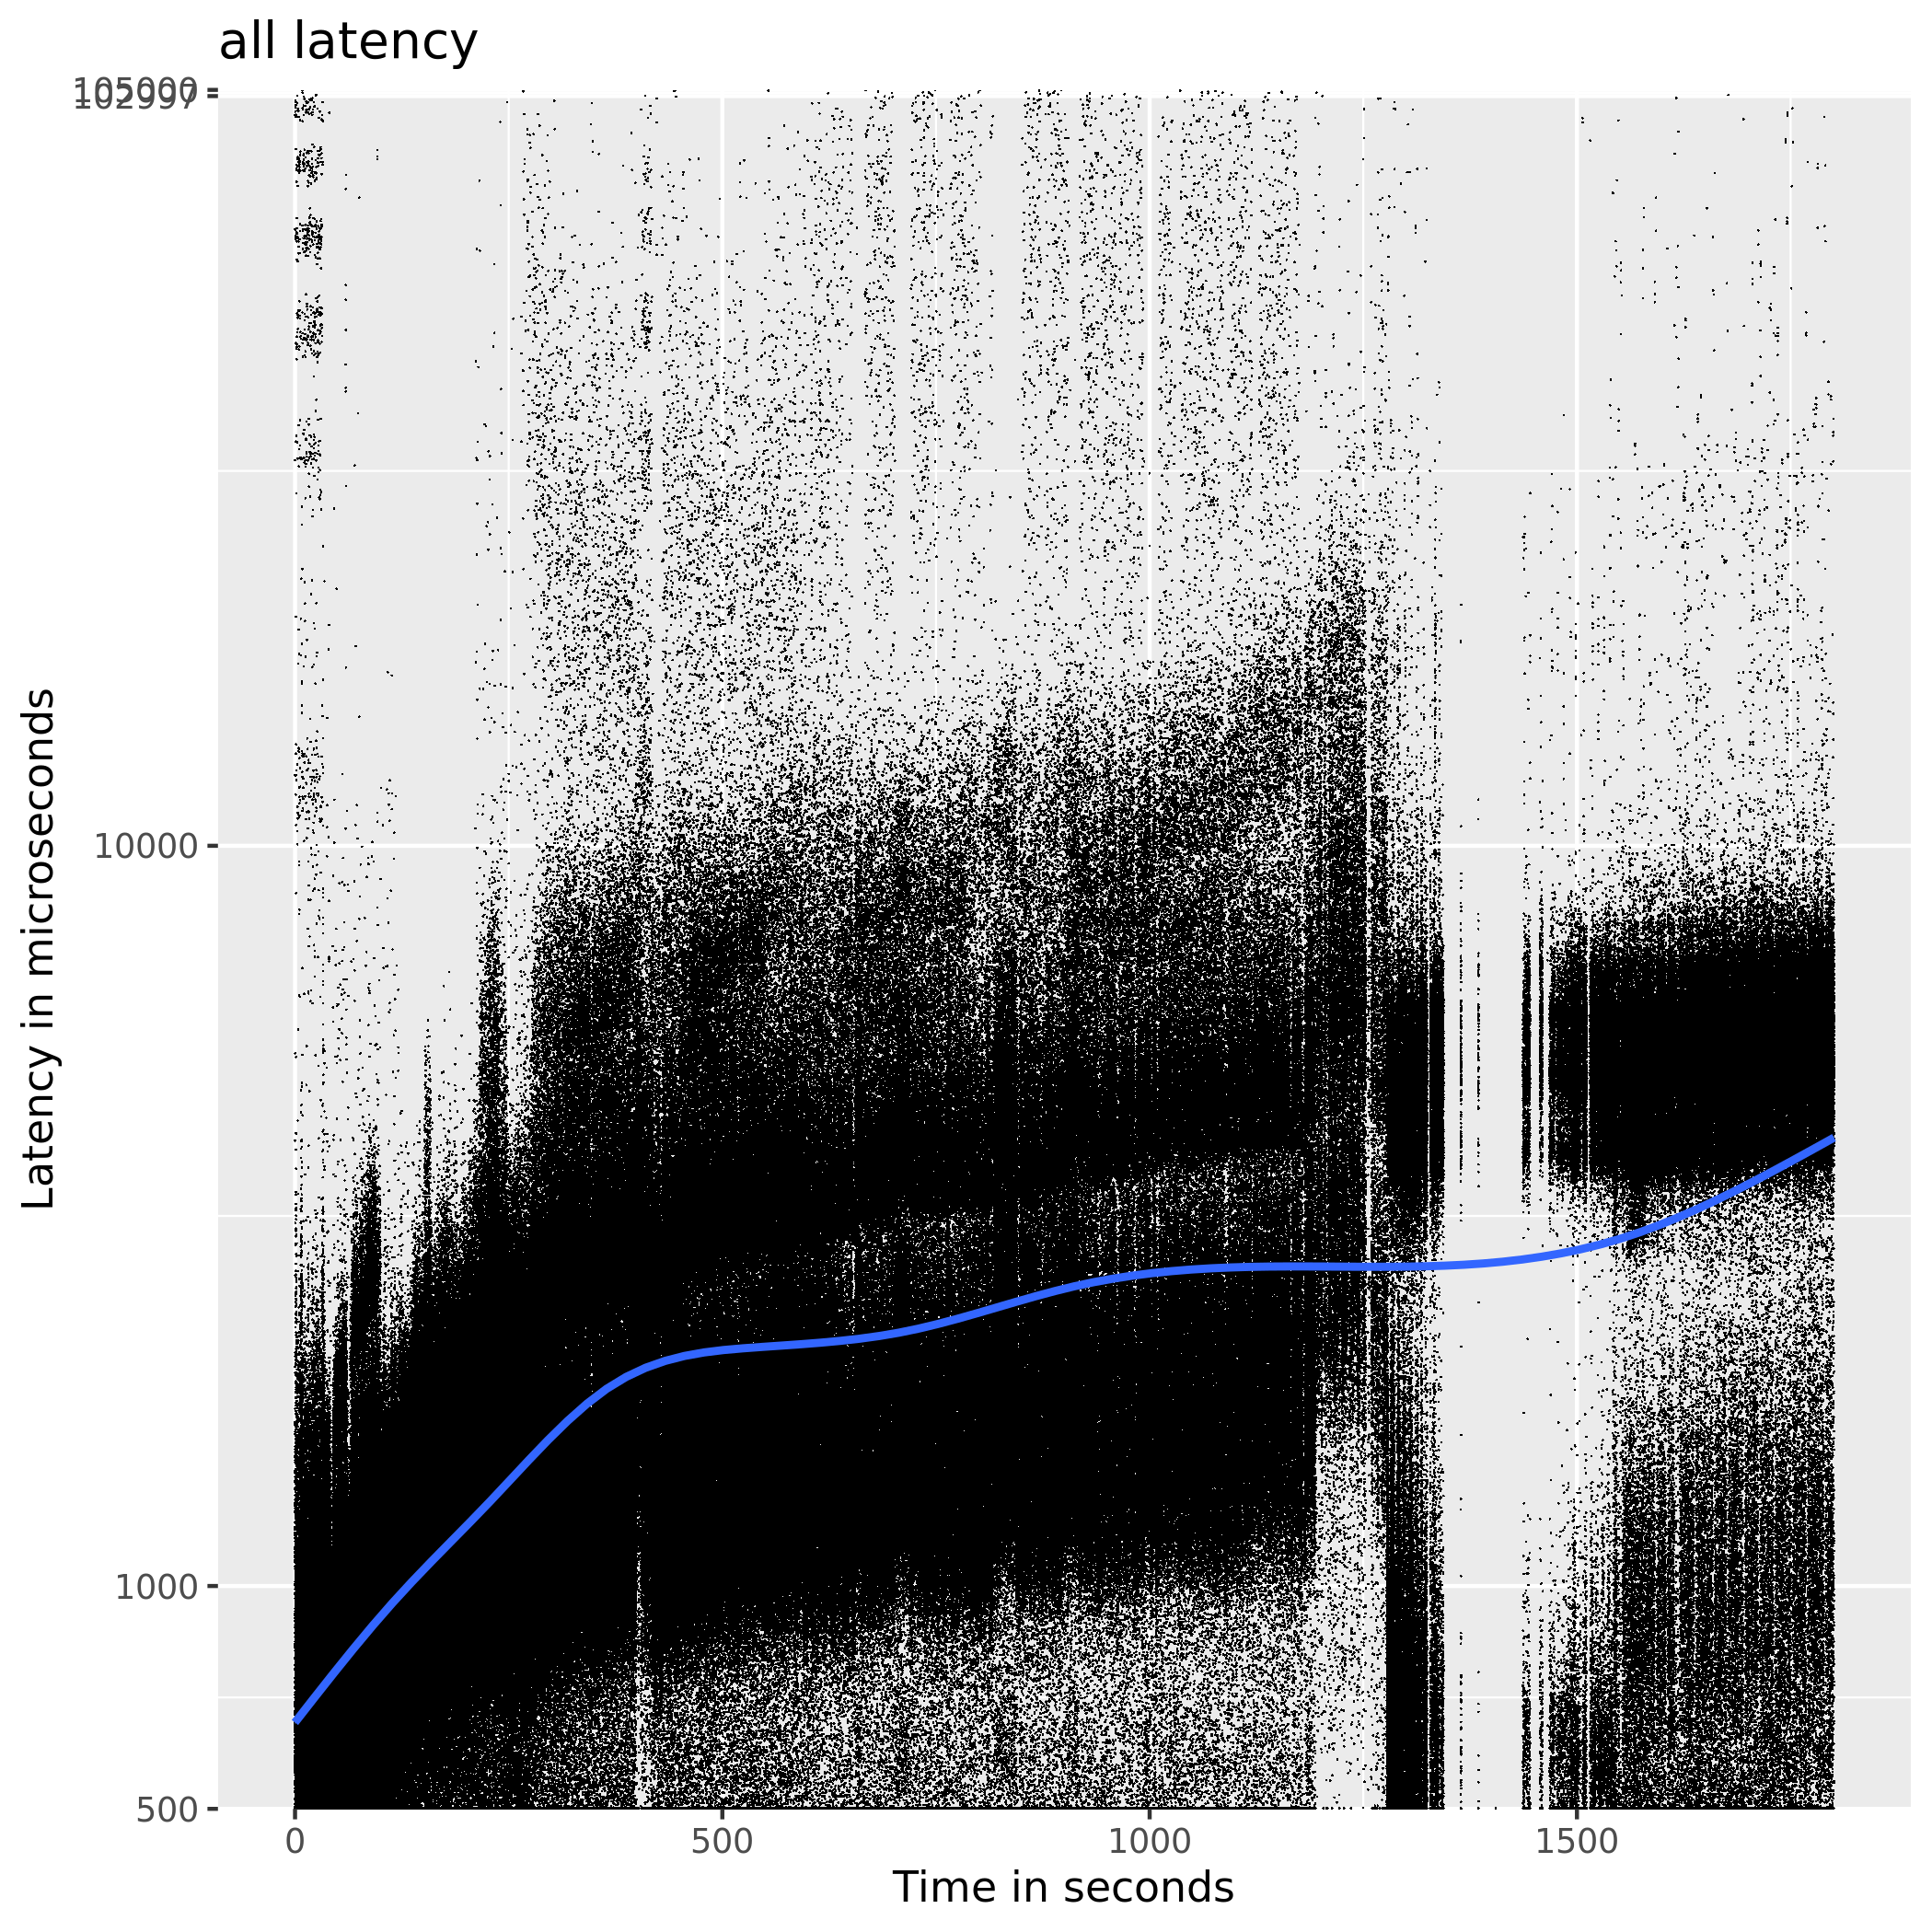
\includegraphics[width=0.5\textwidth]{ConsistentHashing_dynamic_read_heavy_latency}
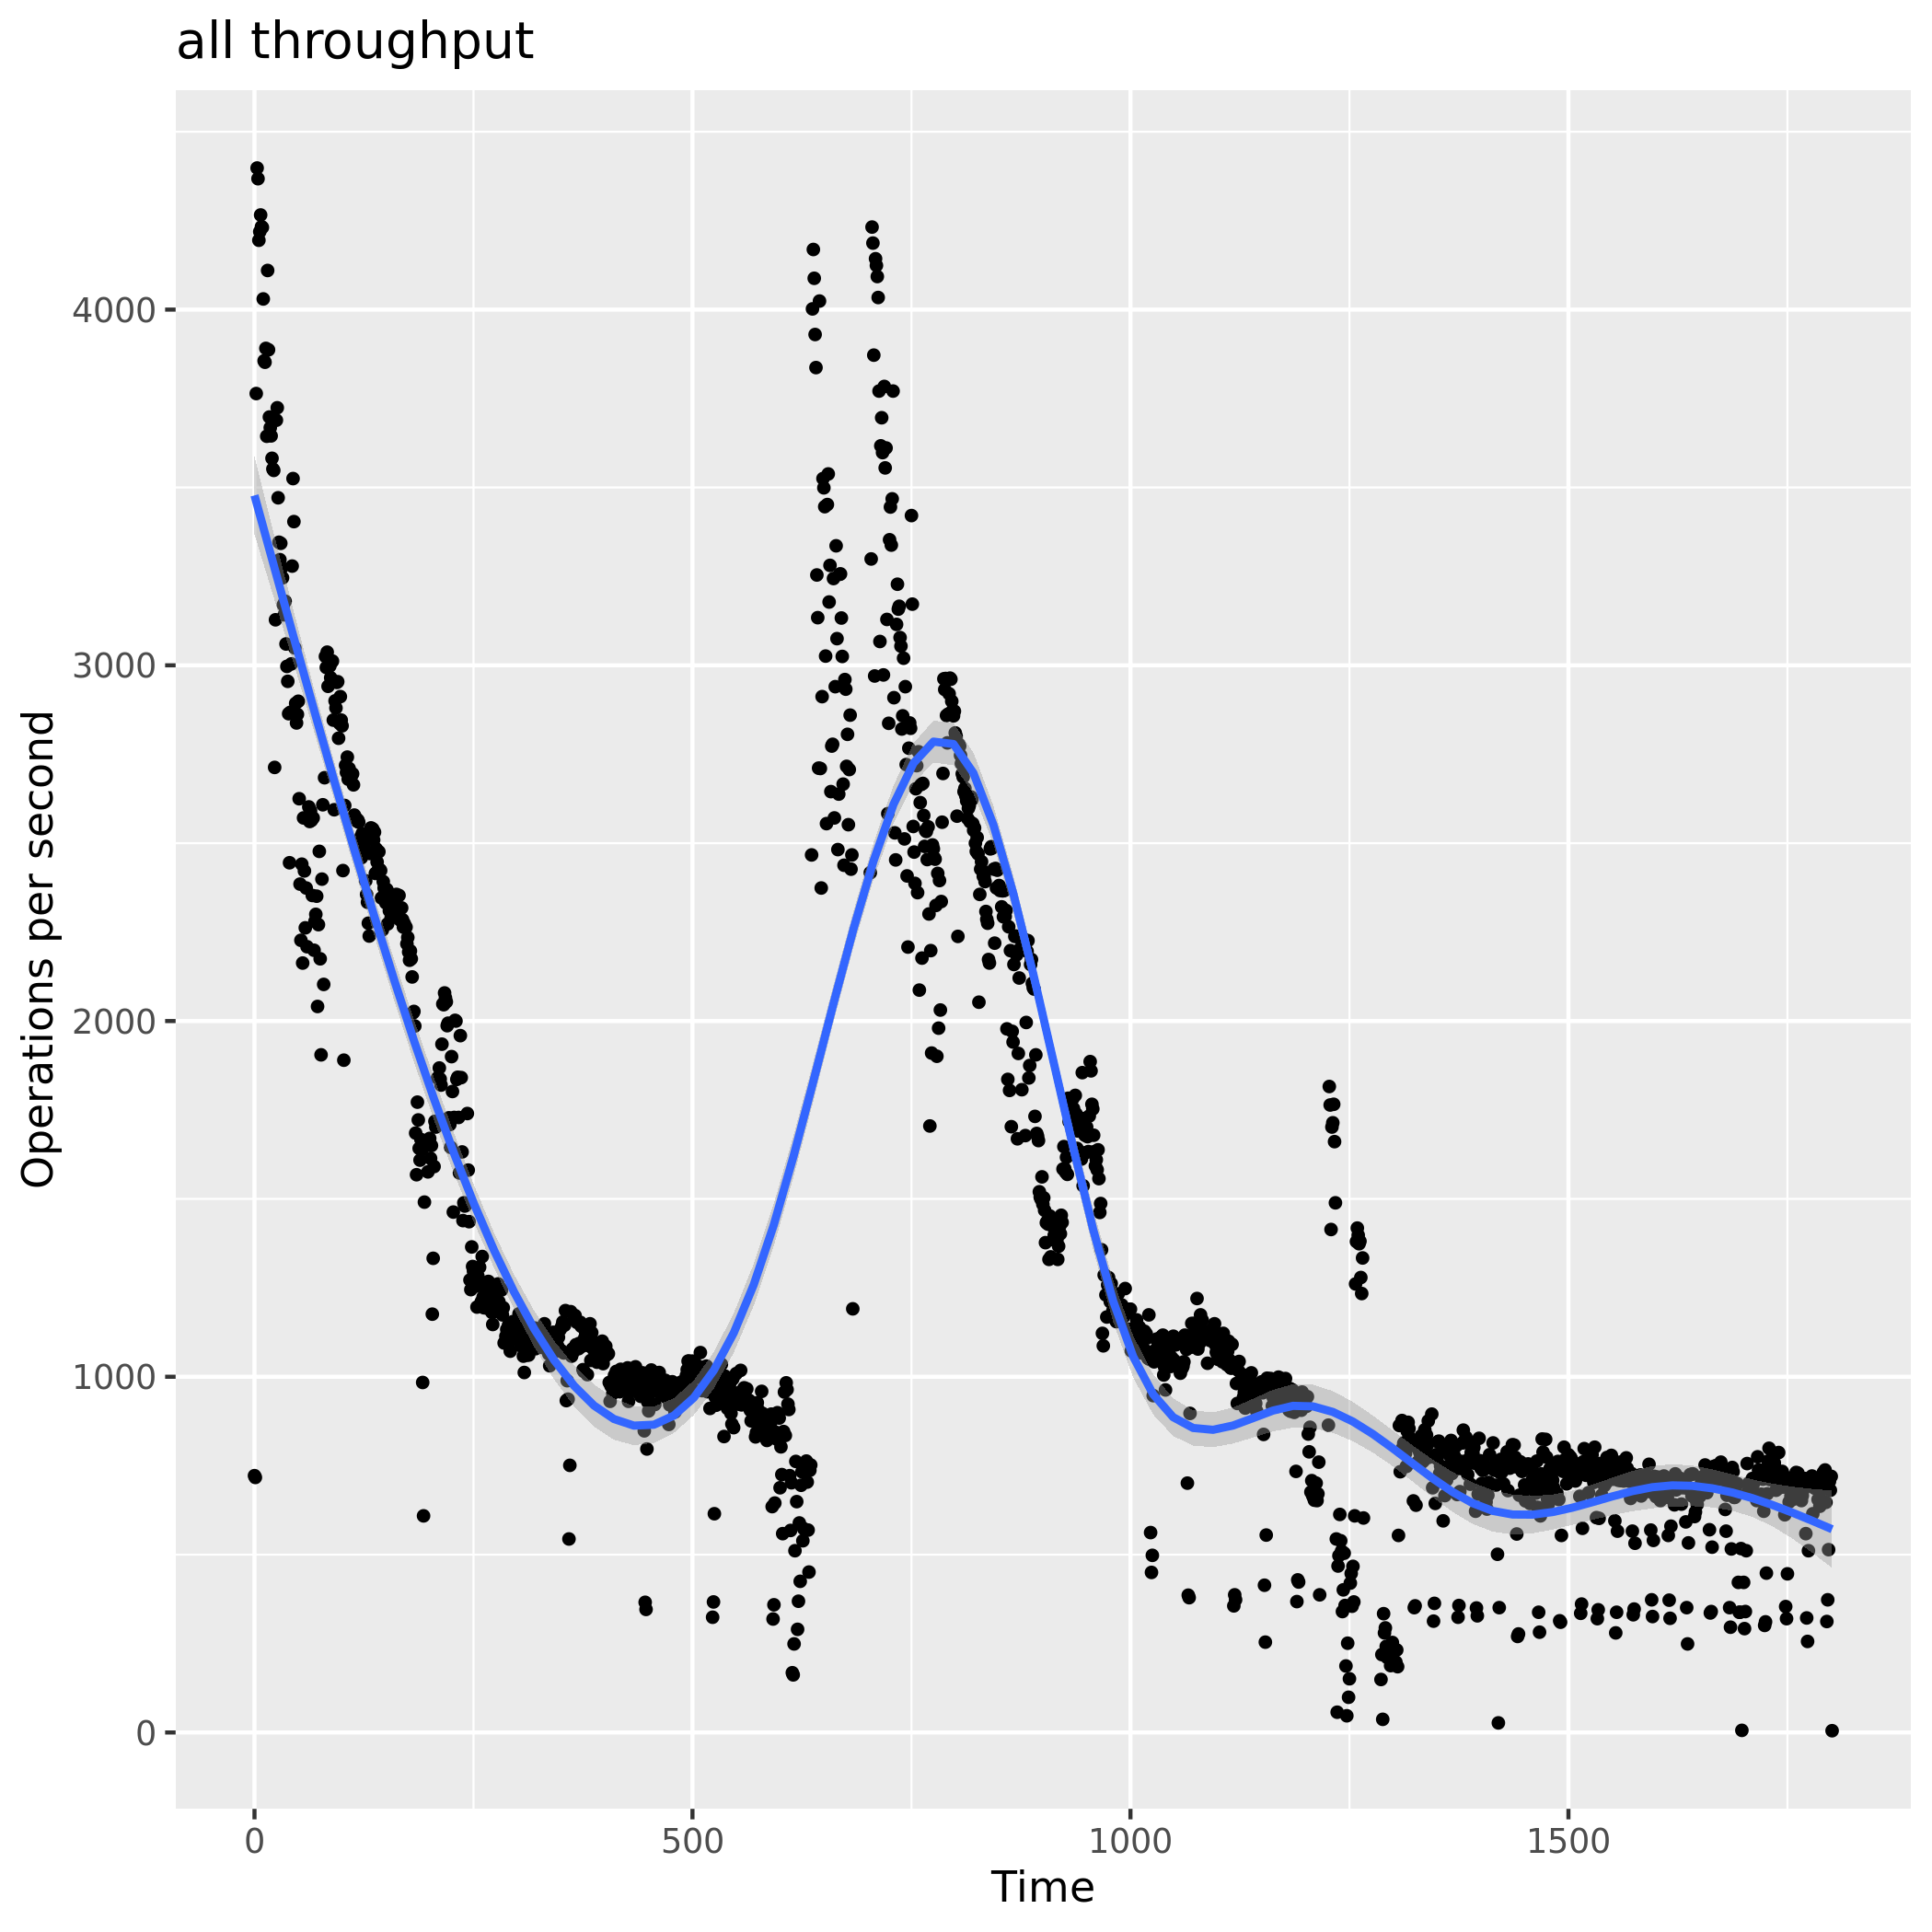
\includegraphics[width=0.5\textwidth]{ConsistentHashing_dynamic_write_heavy_throughput}
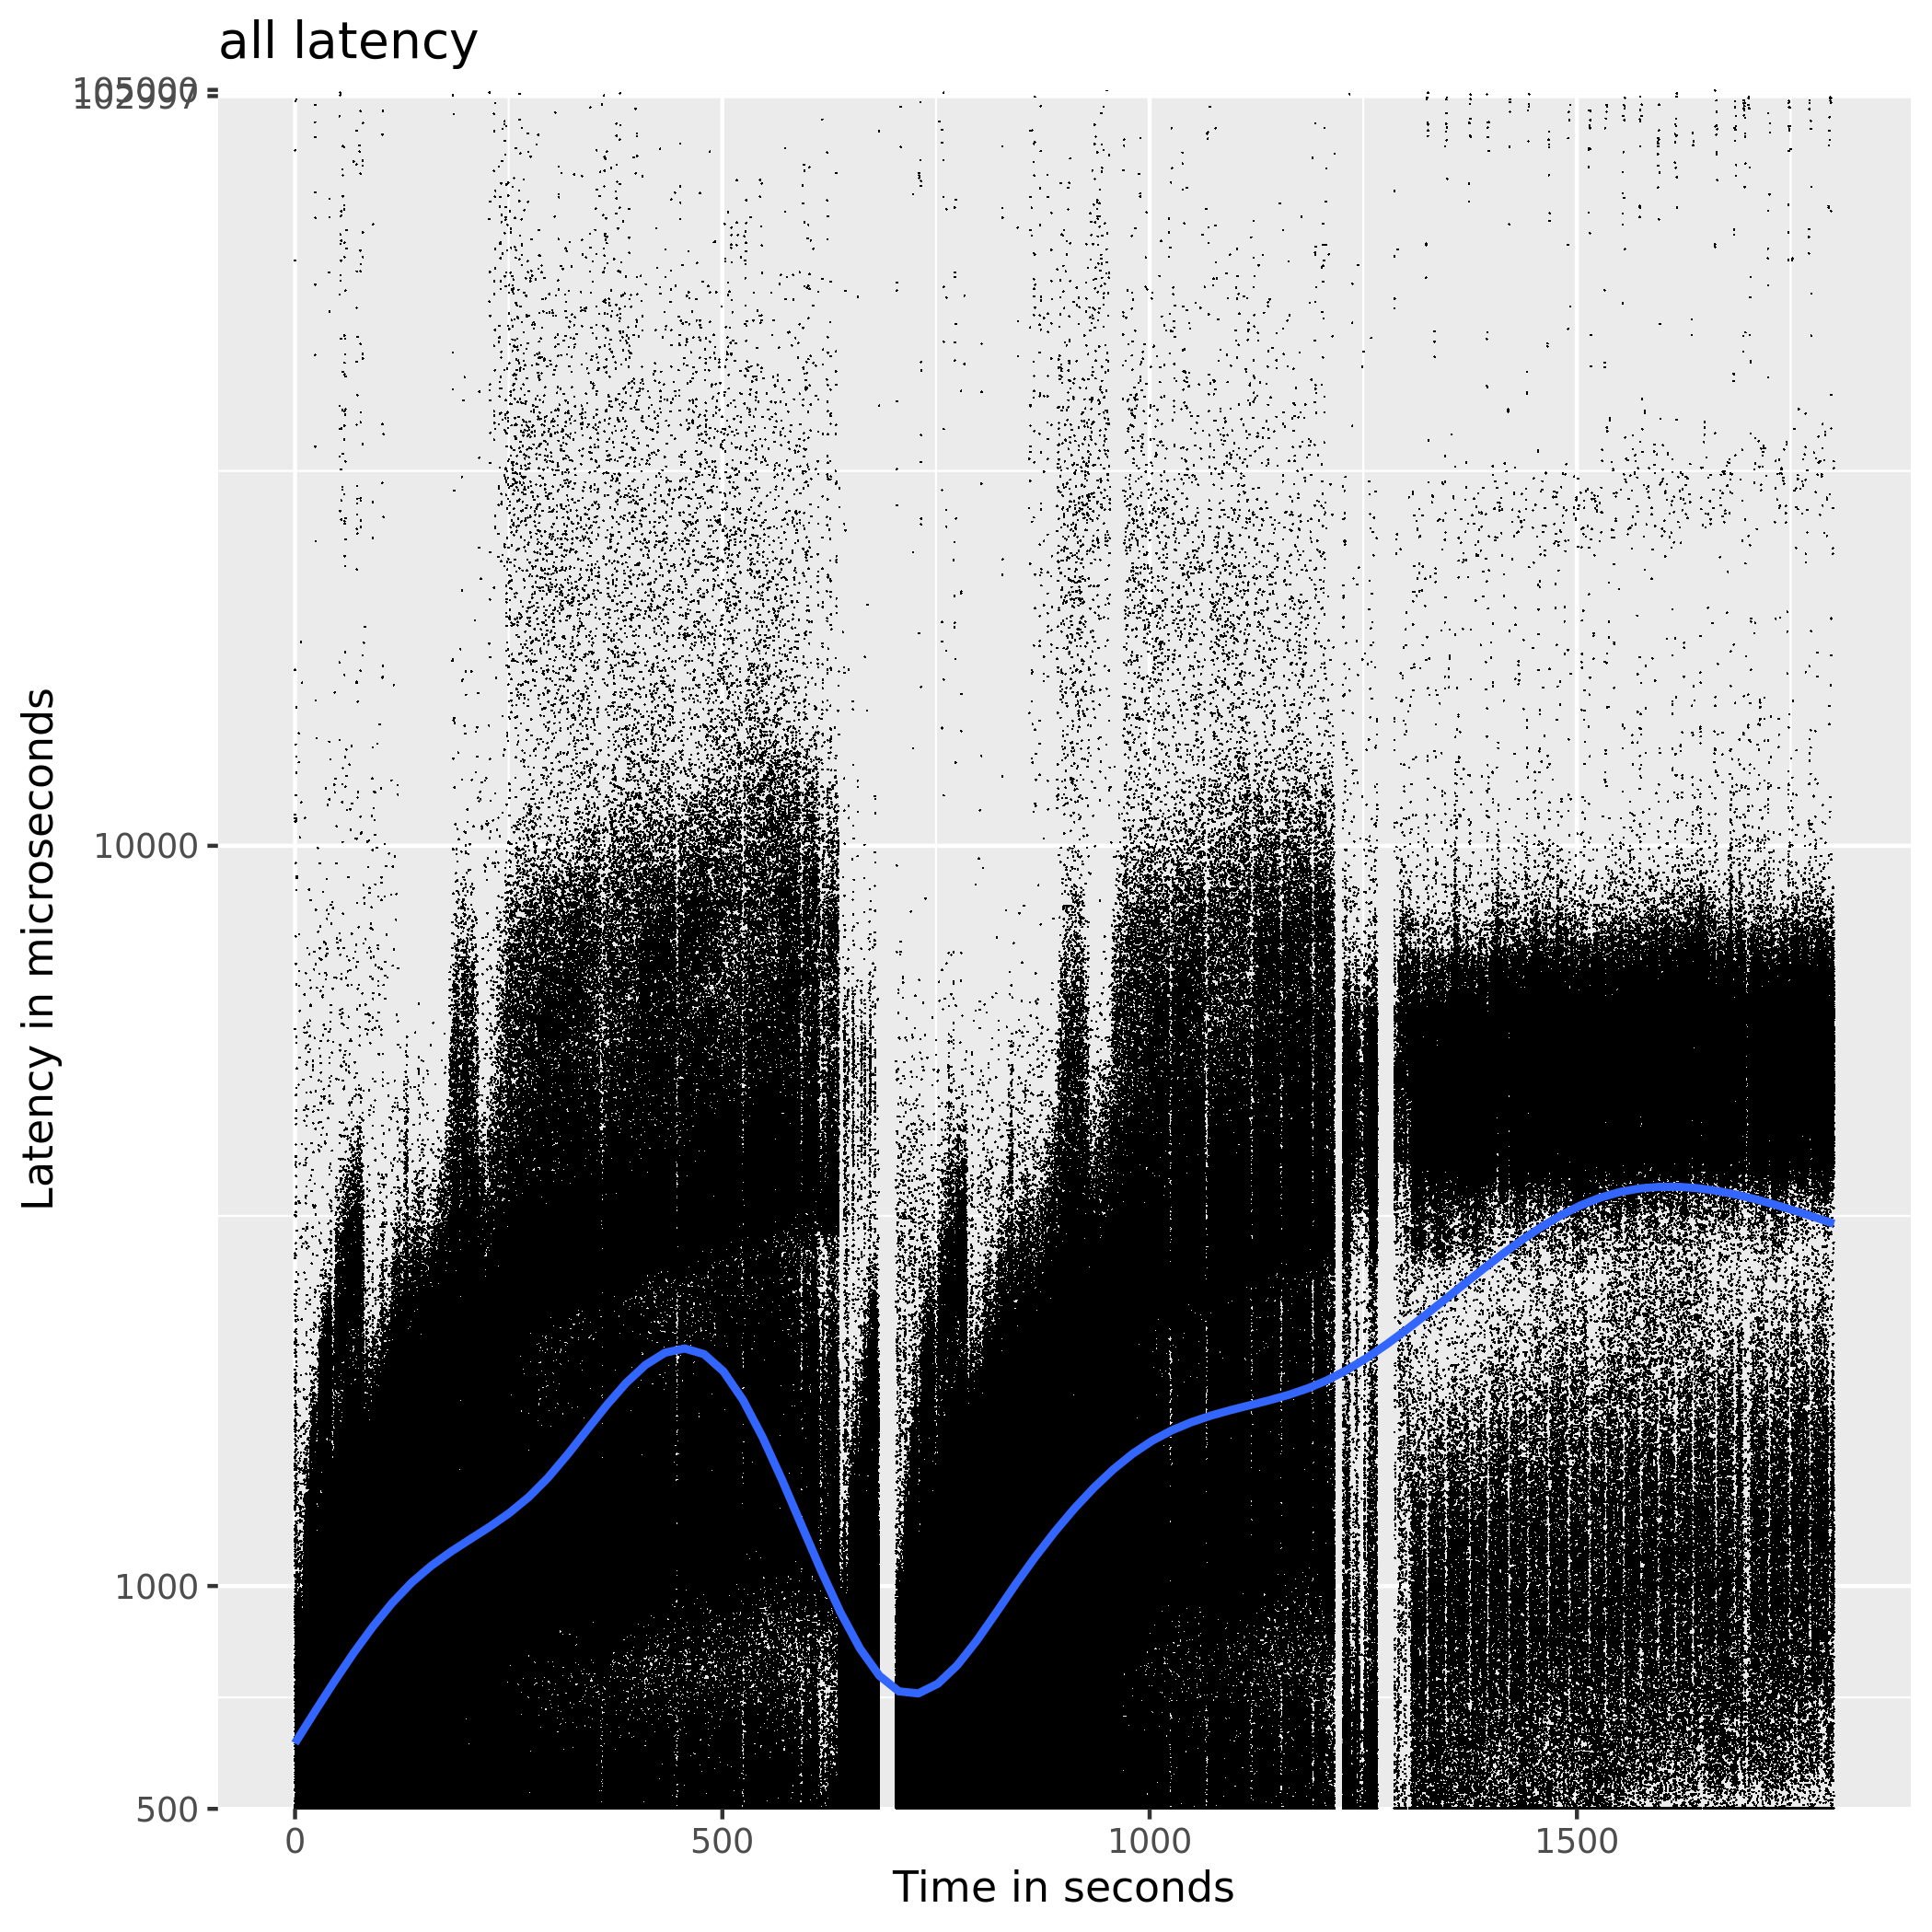
\includegraphics[width=0.5\textwidth]{ConsistentHashing_dynamic_write_heavy_latency}
\caption[Dynamic Runs with Consistent Hashing]{Dynamic Runs with Consistent Hashing. There is a difference how cluster changes influence throughput and latency for read-heavy (top) and write-heavy (bottom) workloads.}
\label{fig:consistent_hashing_dynamic}
\end{figure}
Ignoring the read-heavy dynamic run as an inexplicable anomaly looking at the latency plot for the write-heavy dynamic run seems to show a short impact at 600s and 1200s each that is followed by a longer disruption after a short delay.
Both the phase of initial disruption and the following disruption seem to be longer for the change from C1 to C2.
The initial disruption may be caused by the reconfiguration of the ring and nodes being set to forwarding while the following longer disruption can be explained by the actual handoff operation and potential repair operations.

Regarding the divergence from optimal load balance with Consistent hashing there is an absolute overall average divergence for key load of 0.003821643008703, for put load of 0.032386205130647, and for get load of 0.032384489514972.
The highest divergence is measured with seven nodes in C2 and the lowest in C1 with four nodes.
This is quite intuitive as with four nodes the nodes can be perfectly assigned to the 64 sections of the ring, while with three and seven nodes some nodes have one section more assigned to them than others. 

\subsection{Random Slicing Jumping}
As with Consistent Hashing one cannot see a significant difference between read-heavy and write heavy workloads when looking at the throughput of the system.
A visualization of a run in C0 and C2 is shown in \cref{fig:throughput_random_jumping}.
One can see an influence of the number of nodes in the system on the performance.
This can easily be explained by the higher number of sections and therefore higher lookup time.
In configuration C0 with three nodes the average throughput starts at about 3500 operations per second, steeply decreases to 1000 operations per second at about 450s and from there slowly decreases to 500 operations per second.
The change to four nodes does not significantly change the throughput plot as there are only three new sections on the ring.
However, in configuration C1 with seven nodes the average throughput starts at 1300 and 900 operations per seconds for the read-heavy and write-heavy workload respectively and then decreases for both cases to 500 operations per second.
\begin{figure}
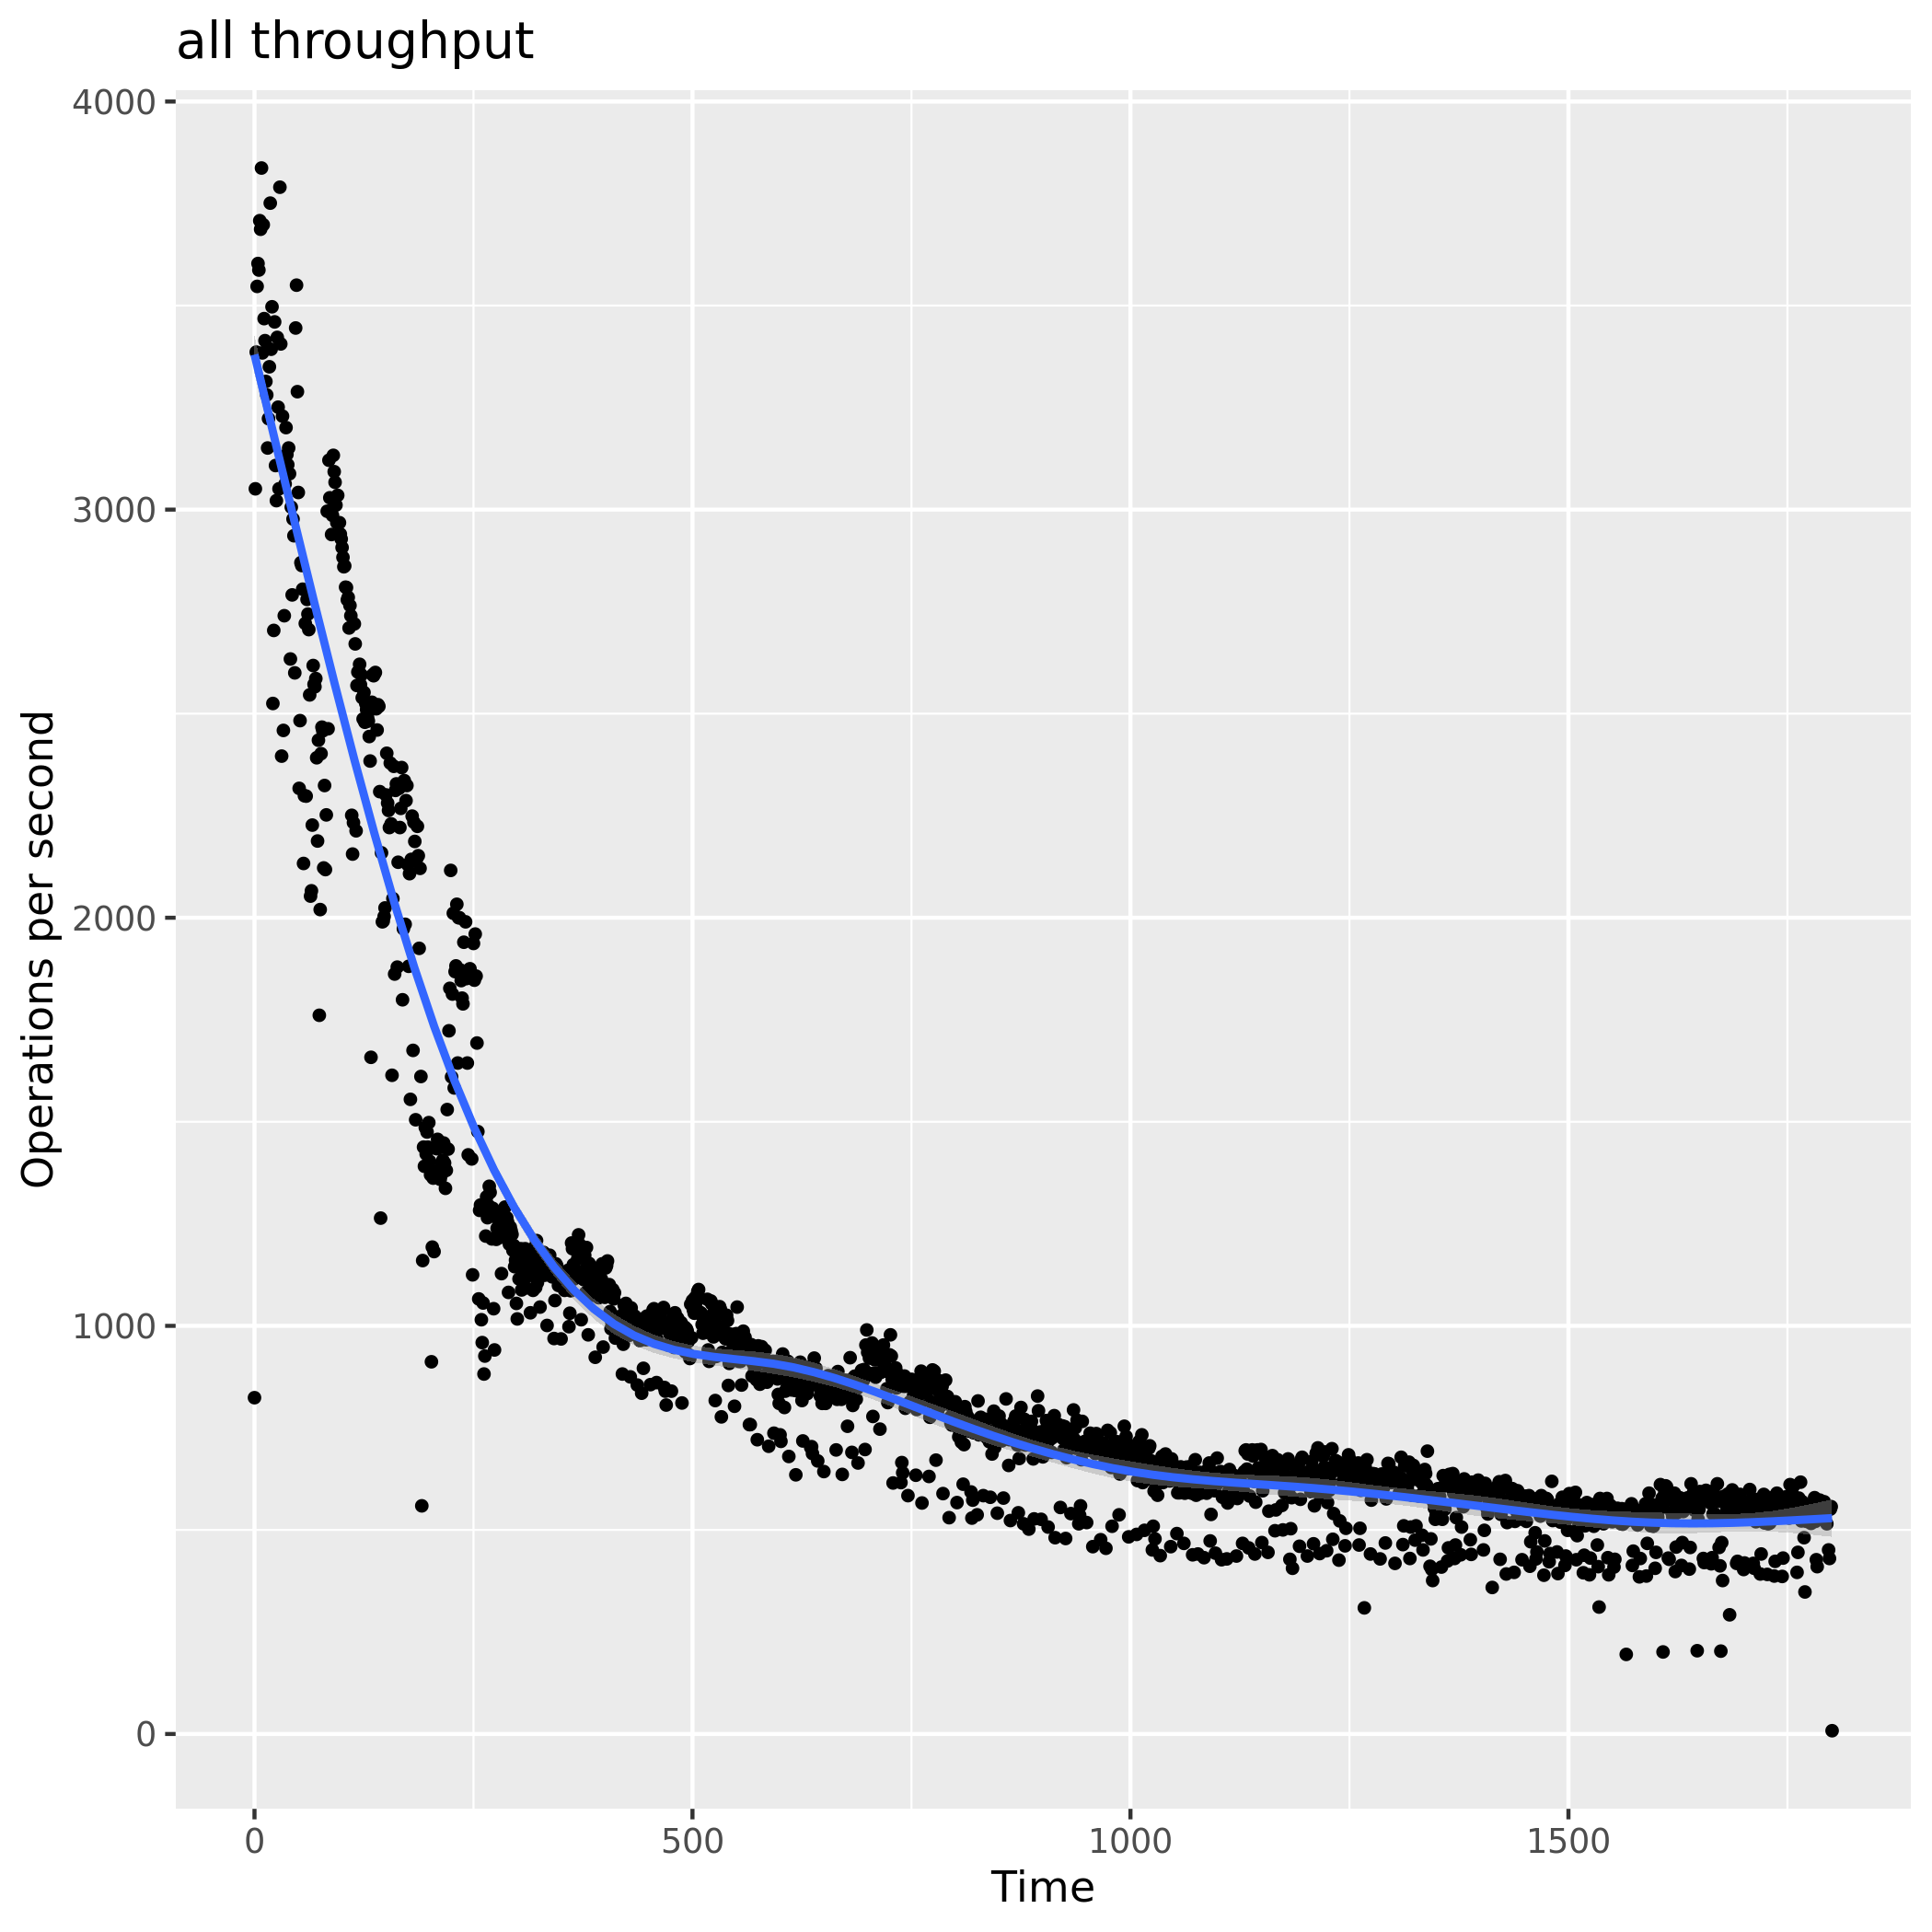
\includegraphics[width=0.5\textwidth]{RandomSlicing_Jumping_C0_write_heavy_throughput}
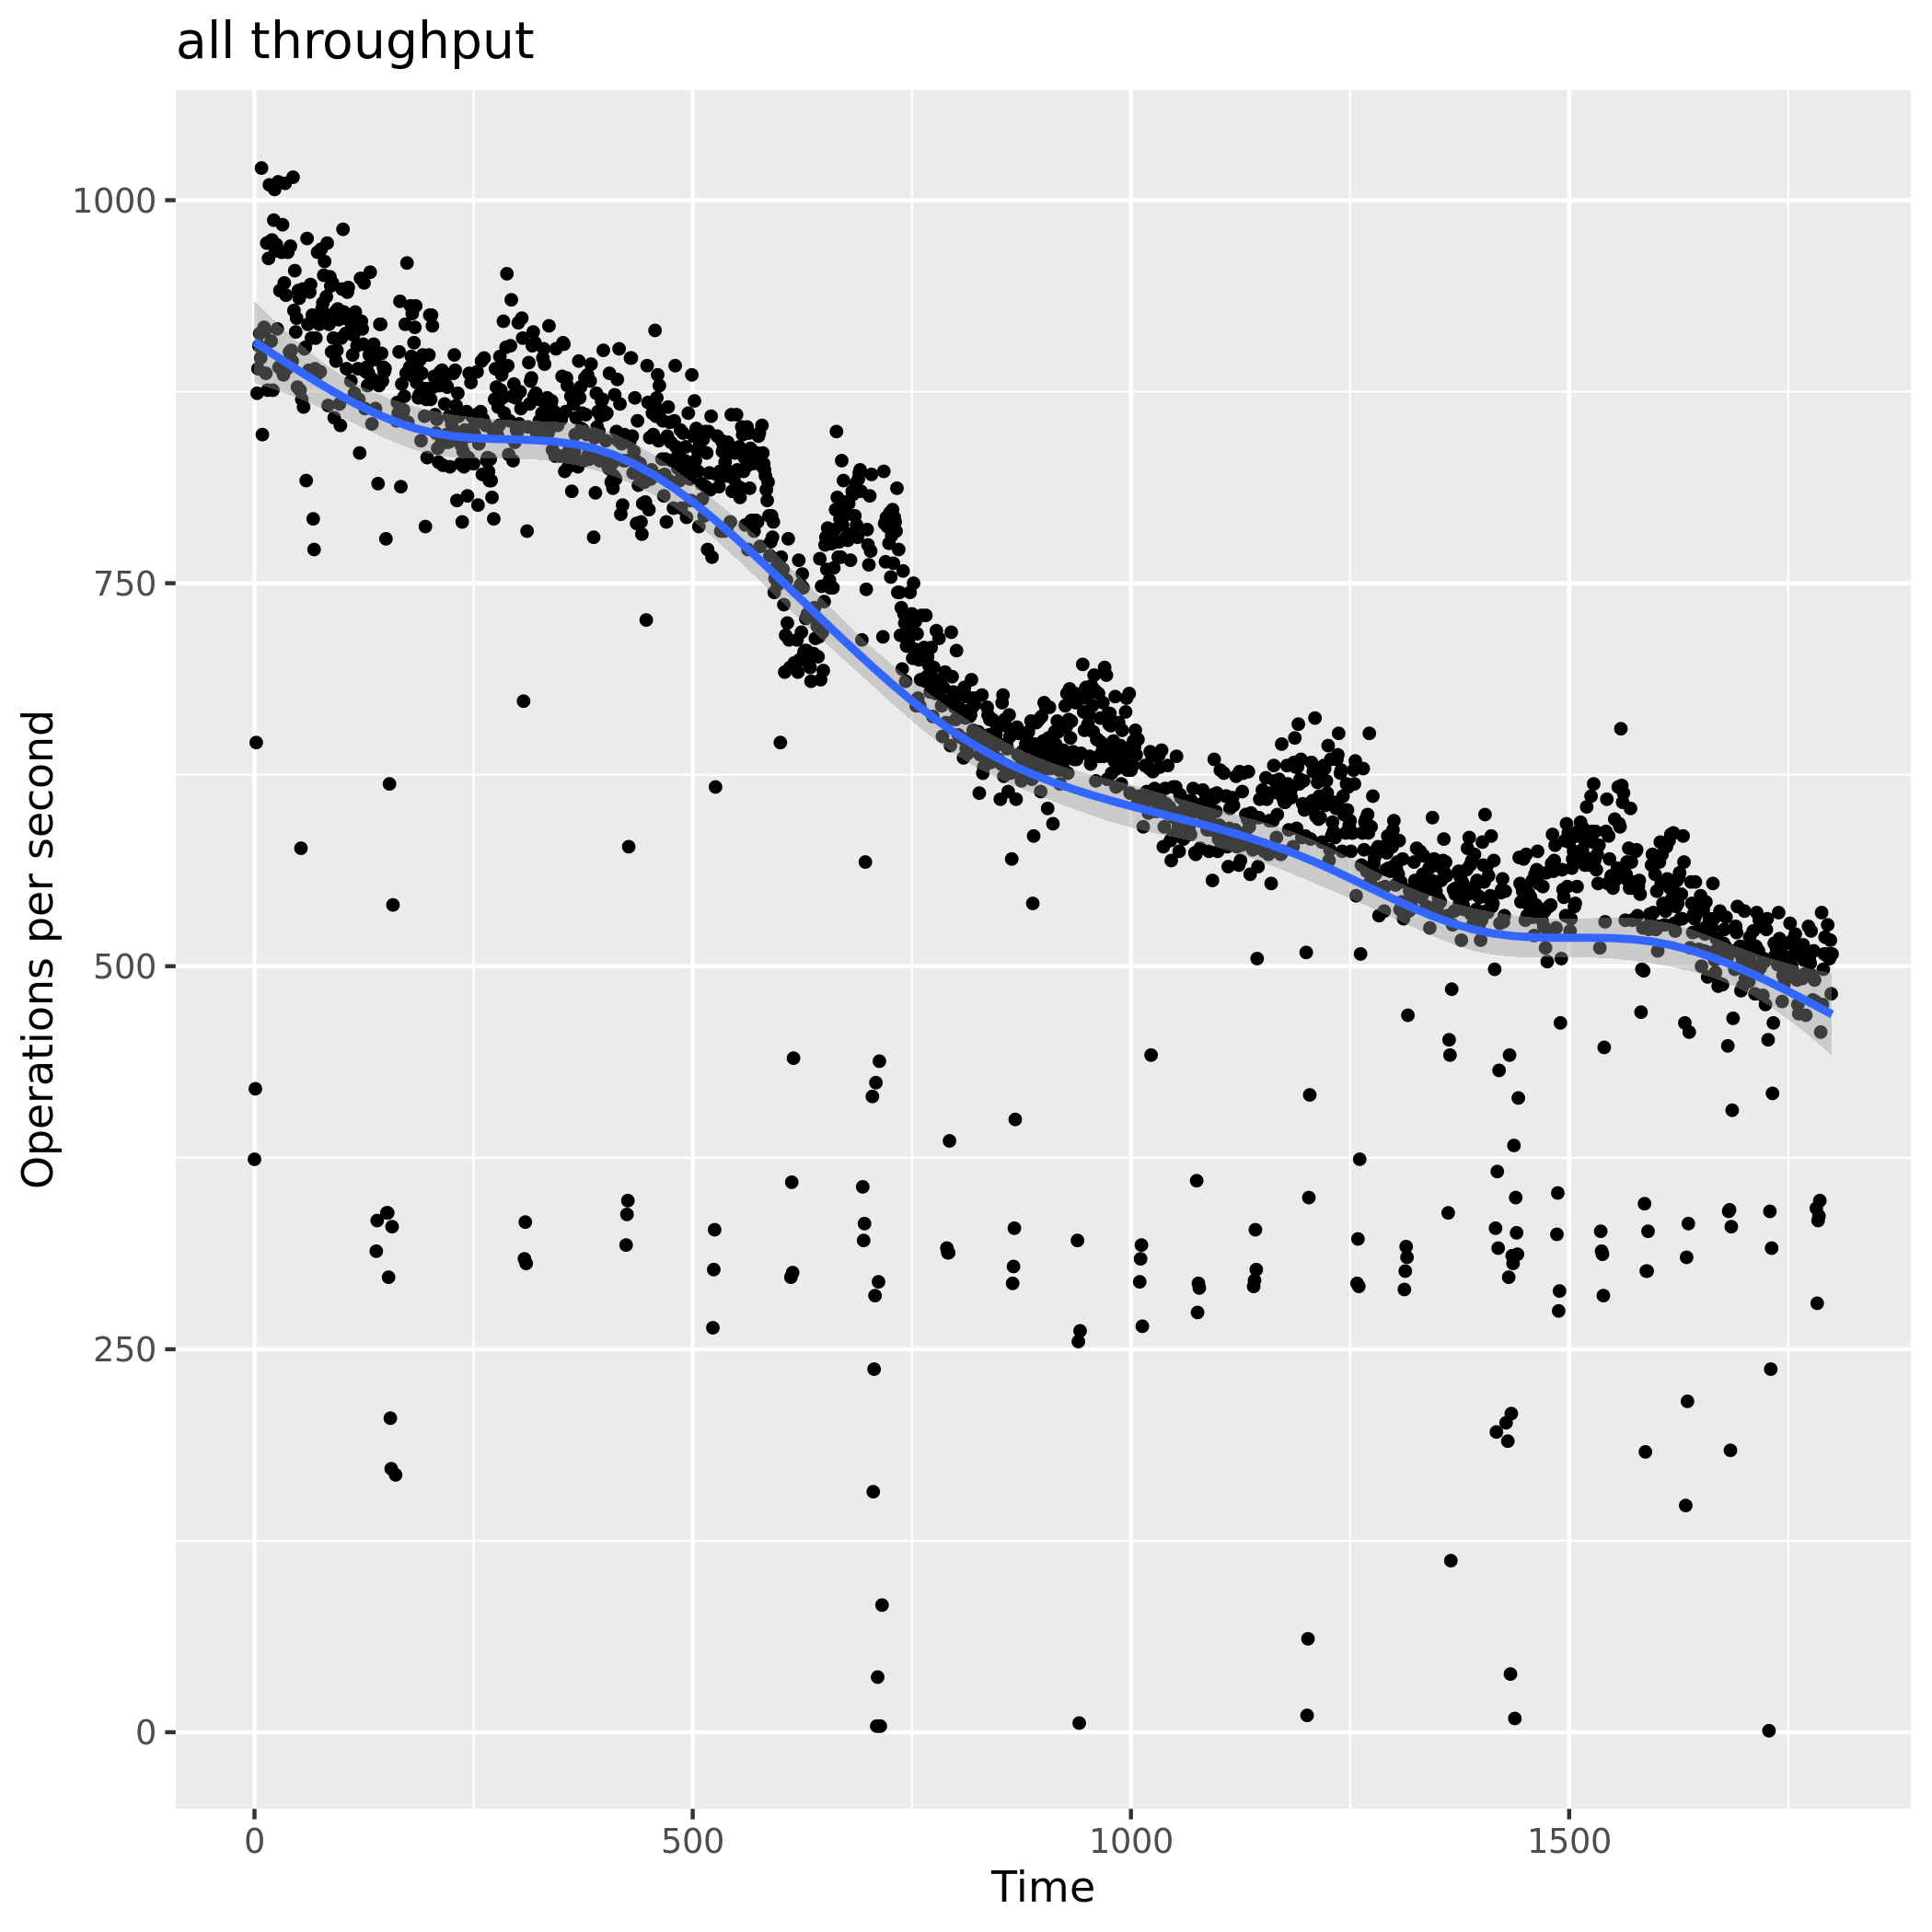
\includegraphics[width=0.5\textwidth]{RandomSlicing_Jumping_C2_write_heavy_throughput}
\caption[\ac{RS} with Ring Jumping Throughput Comparison]{\ac{RS} with Ring Jumping Throughput Comparison. Showing the throughput for \ac{RS} with Ring Jumping in C0 and C2 with write-heavy workload.}
\label{fig:throughput_random_jumping}
\end{figure}

In the dynamic benchmark runs the decrease in throughput after each configuration change is in accordance with the values measured for those configurations in the static run.
An exemplary visualization of the write-heavy dynamic run is shown in \cref{fig:random_slicing_jumping_dynamic}.
Just before the change from C0 to C1 the throughput is at about 1000 operations per second which is the same as just before the change from C1 to C2.
At the end of the run the throughput decreased to about 550 operations per second.
There is a clear edge in the latency plot at the 600s and 1200s mark but there is no visible phase of disruption which implies that there is not a long phase of handoff operations.
\begin{figure}
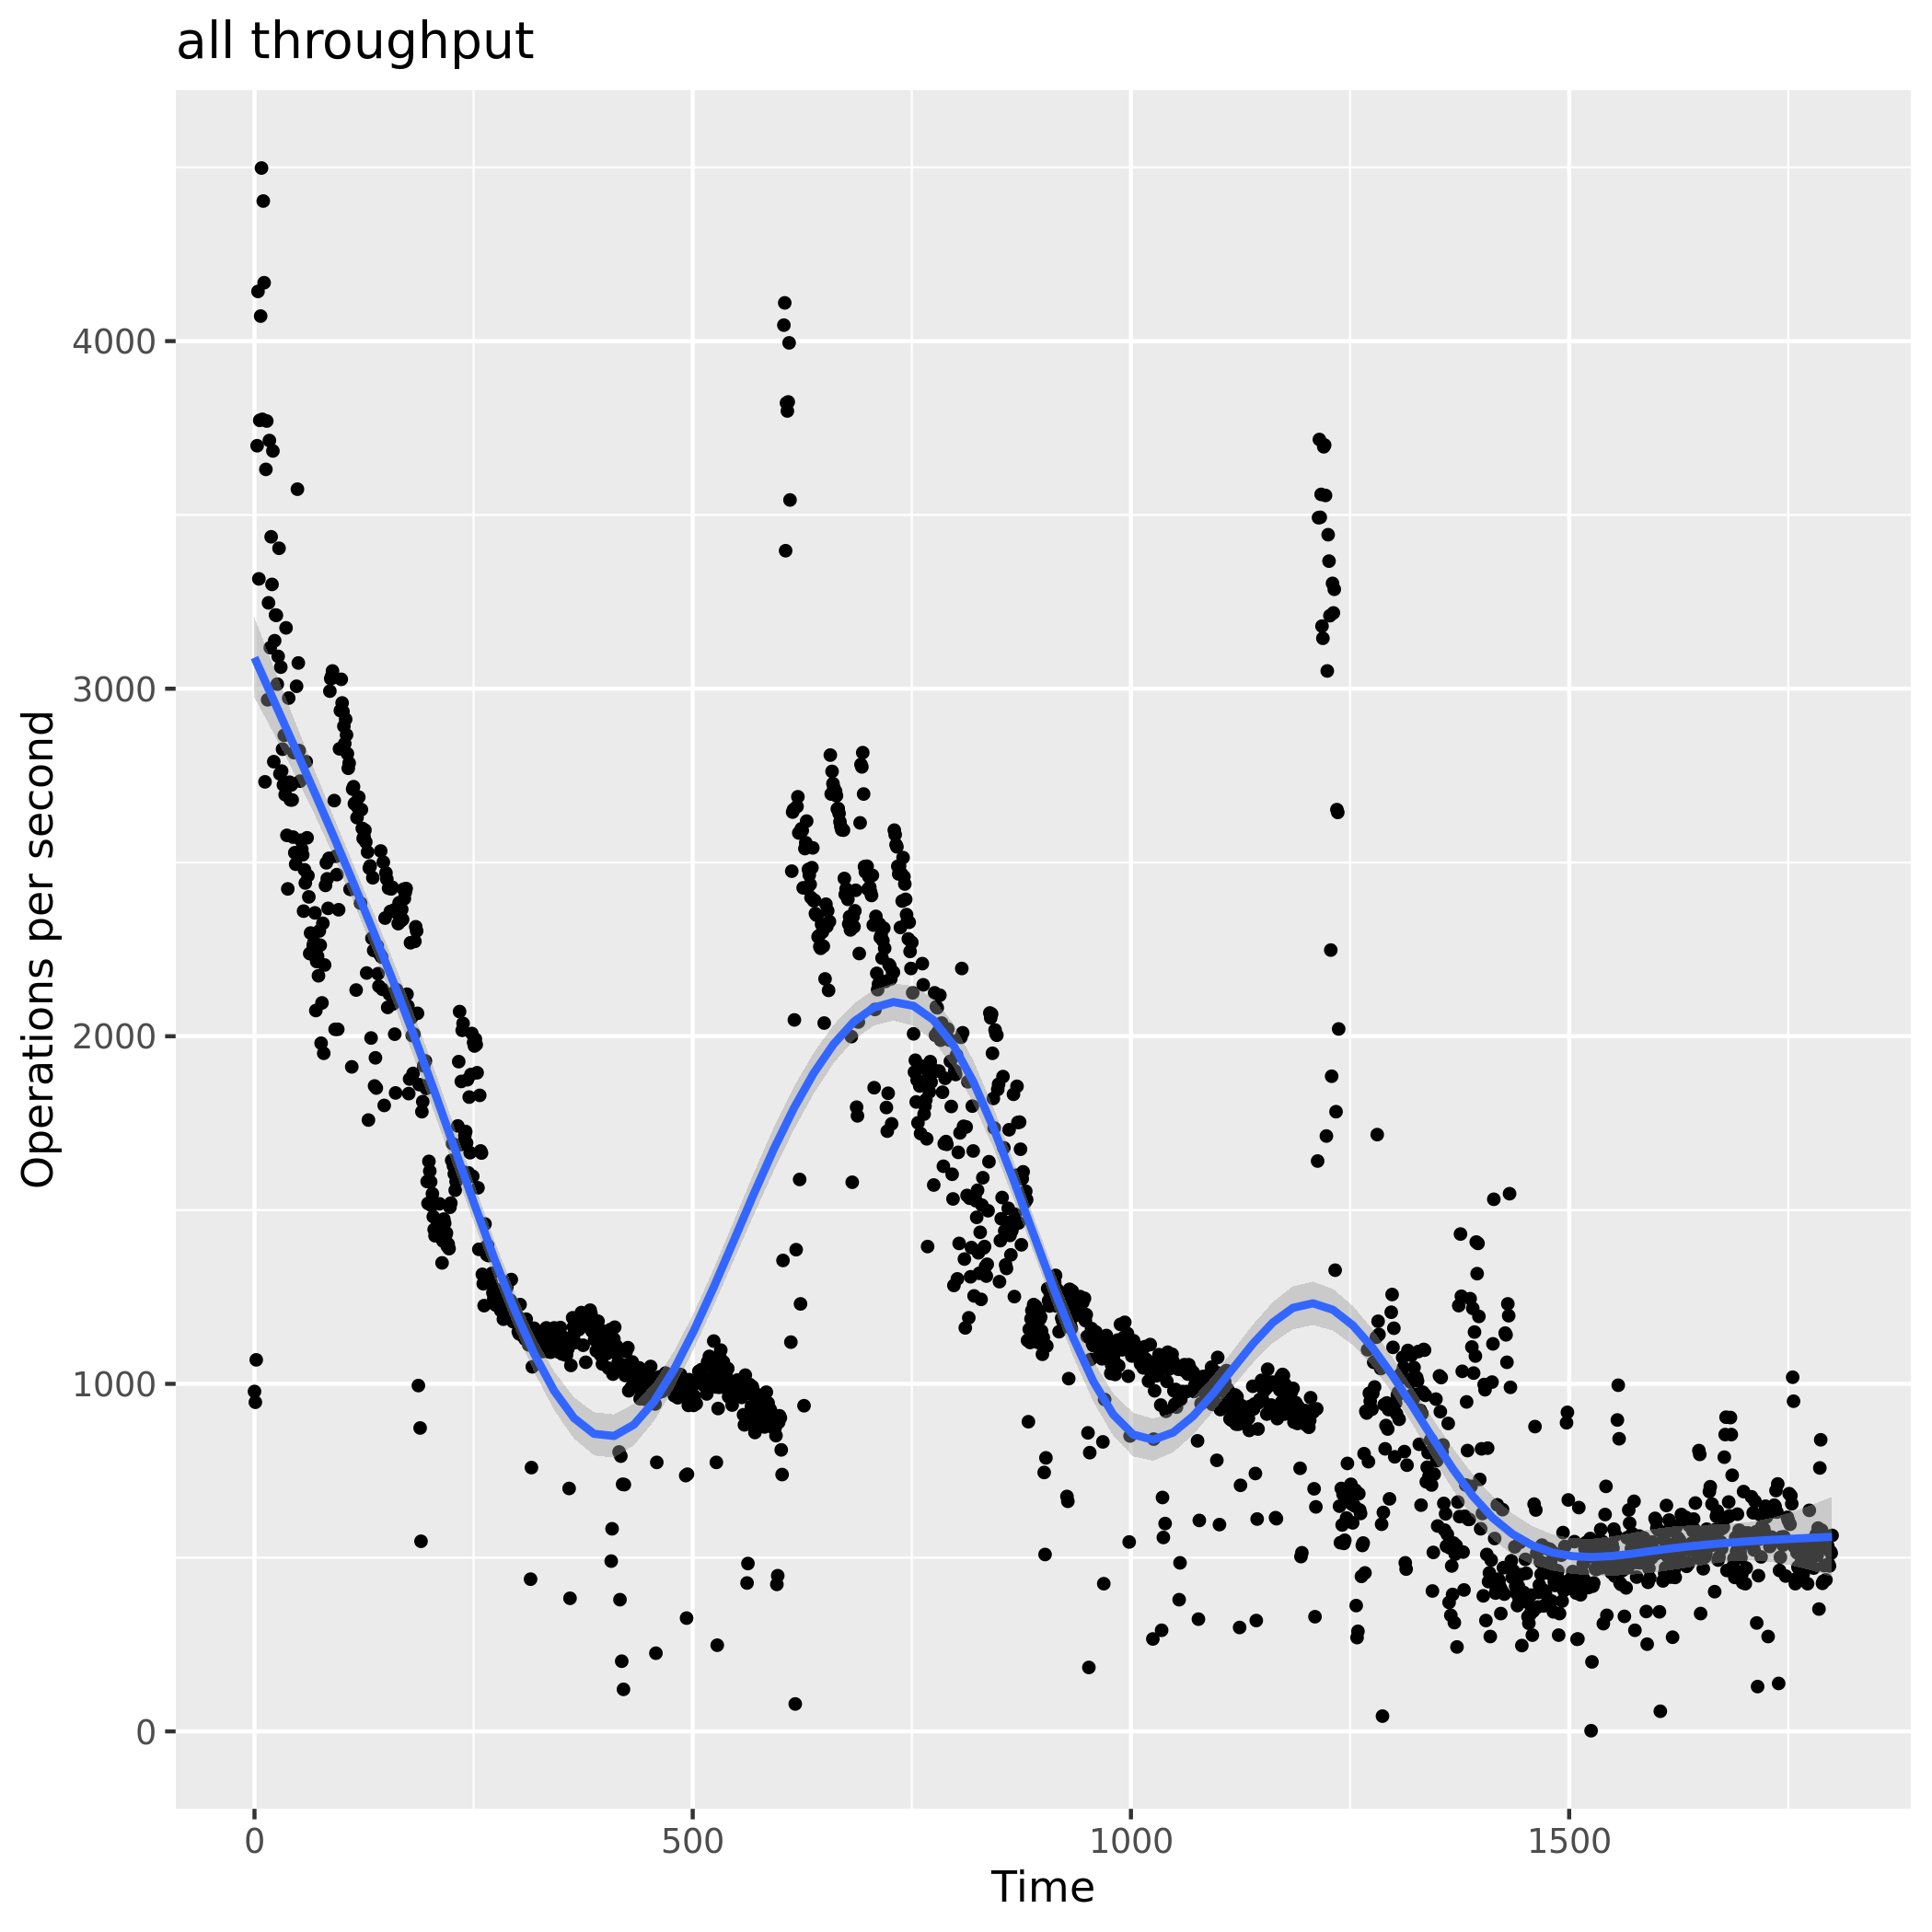
\includegraphics[width=0.5\textwidth]{RandomSlicing_Jumping_dynamic_write_heavy_throughput}
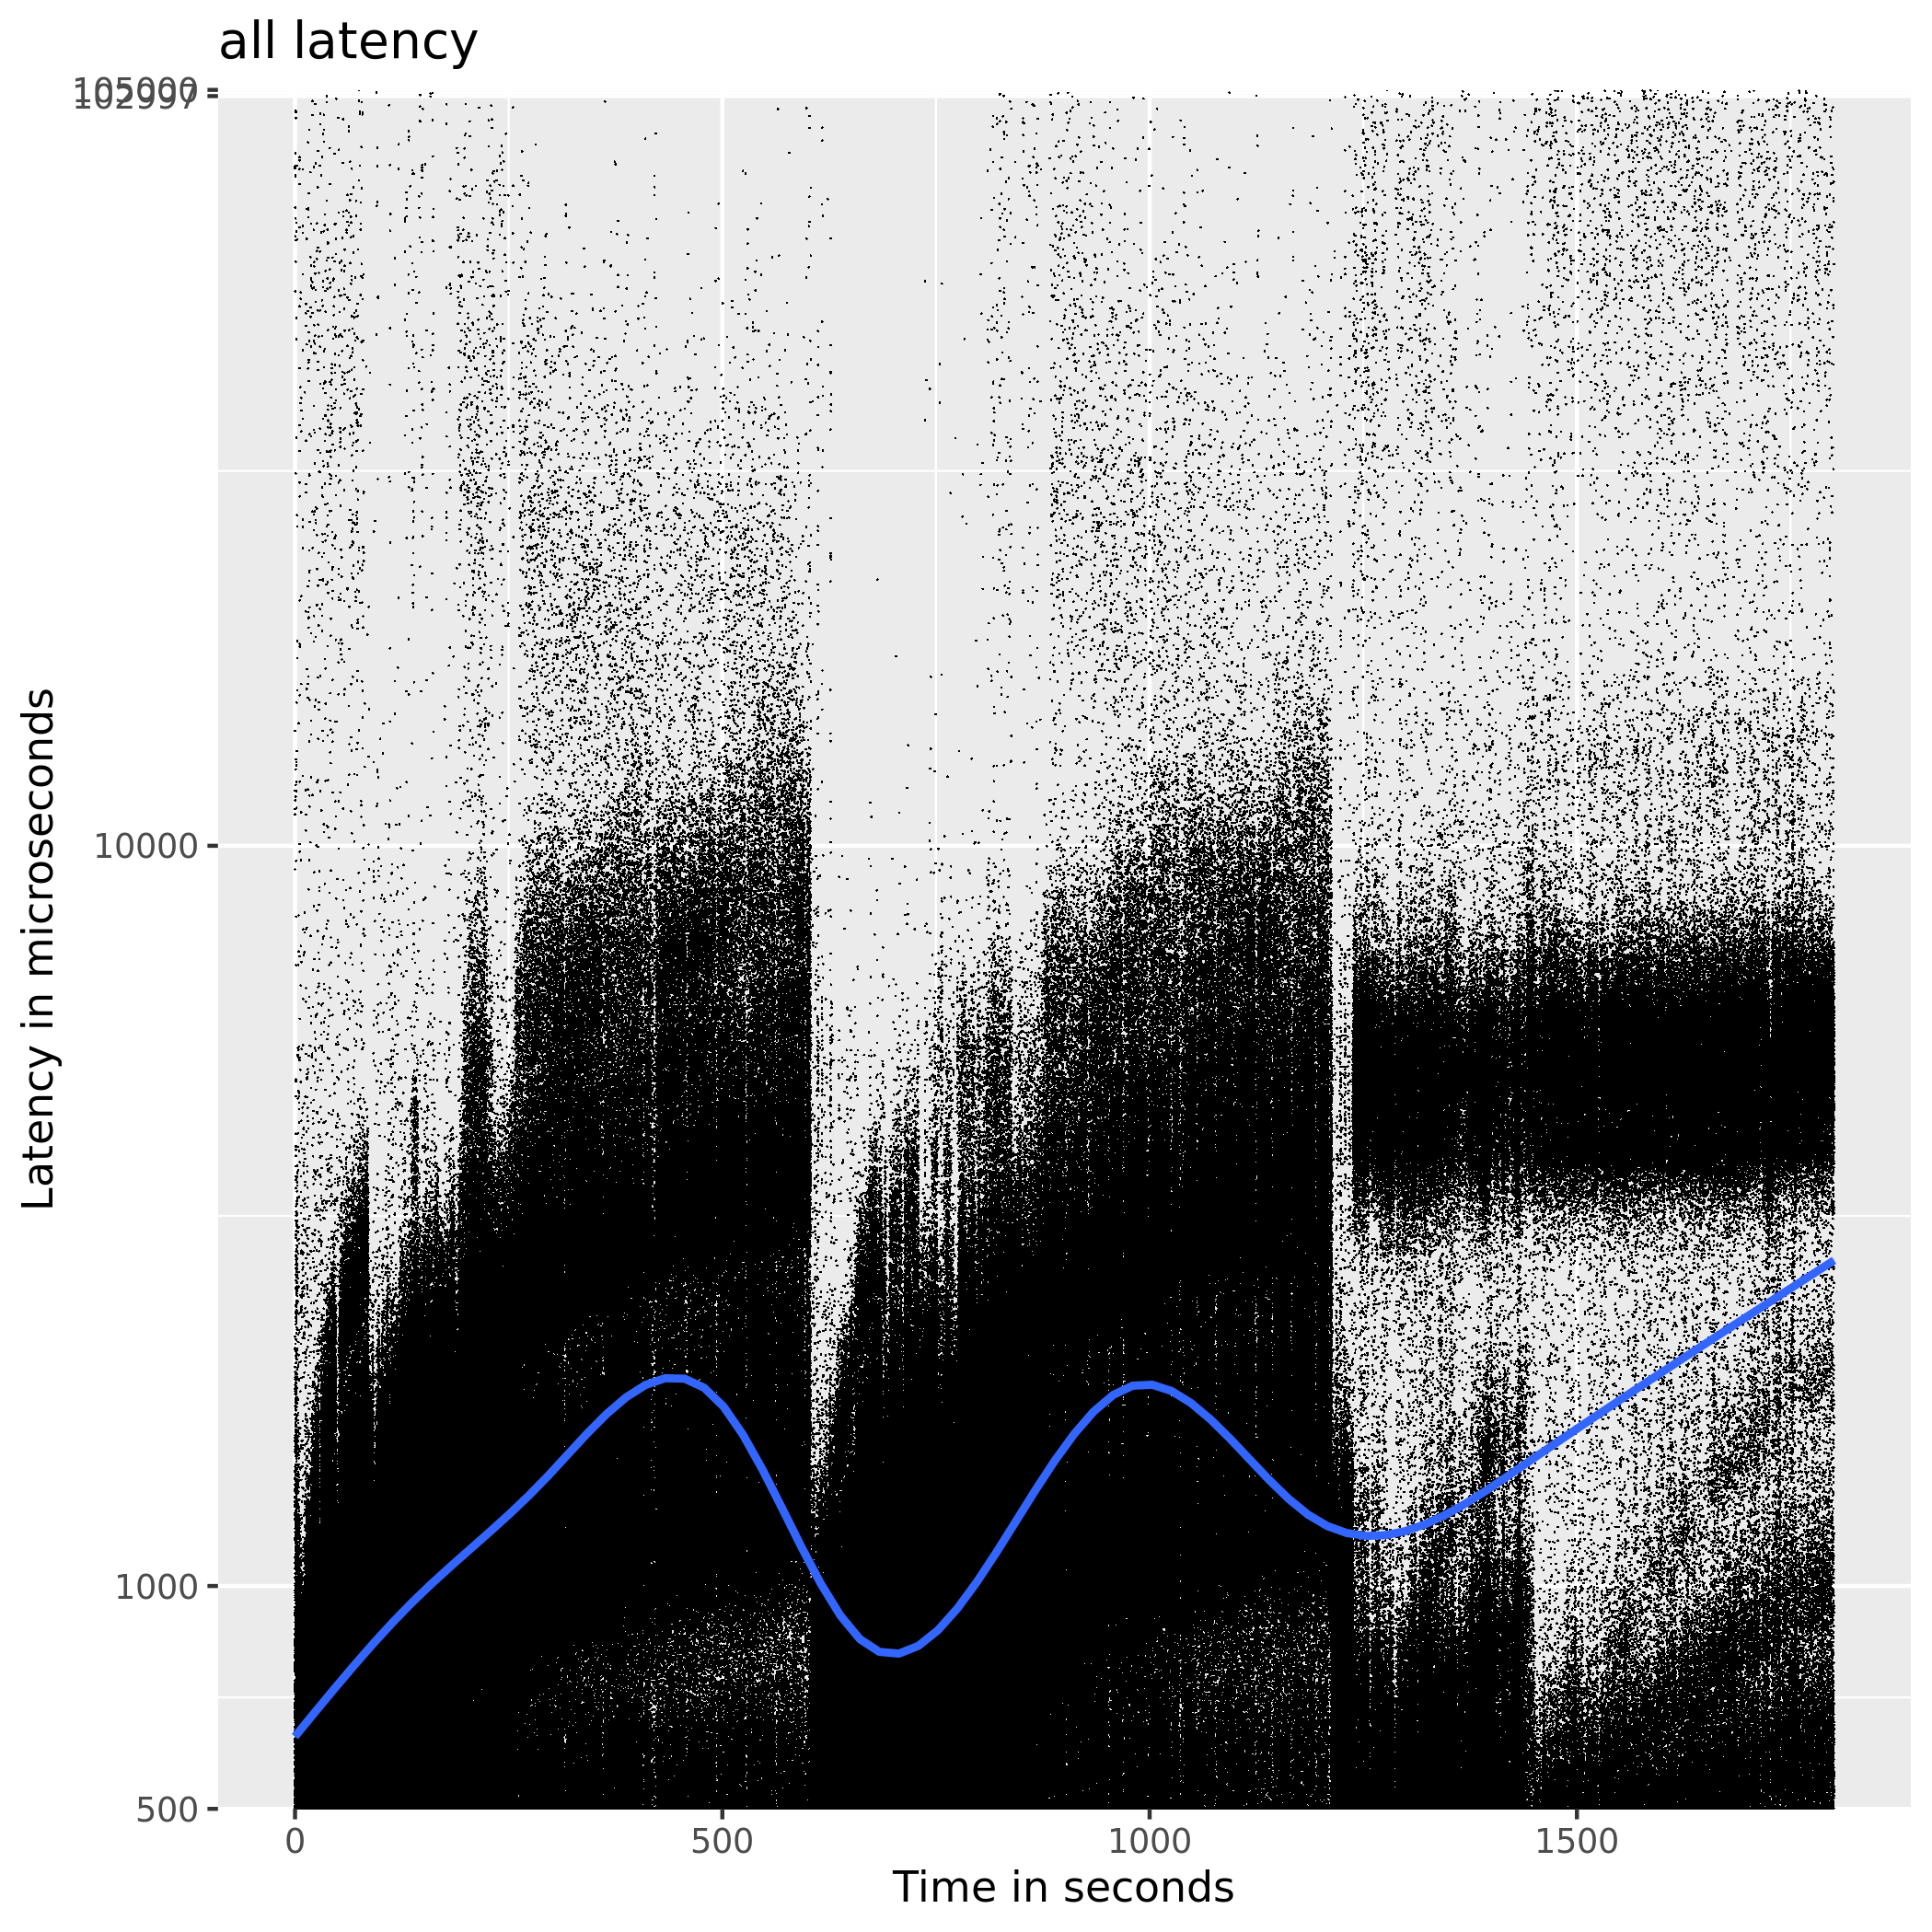
\includegraphics[width=0.5\textwidth]{RandomSlicing_Jumping_dynamic_write_heavy_latency}
\caption[Dynamic Run with \ac{RS} and Ring Jumping]{Dynamic Runs with \ac{RS} and Ring Jumping.}
\label{fig:random_slicing_jumping_dynamic}
\end{figure}

Regarding the divergence from optimal load balance with \ac{RS} and Ring Jumping there is an absolute overall average divergence for key load of 0.0303095841515983, for put load of 0.036558287305248, and for get load of 0.03657058797636.
Ignoring C0 with exactly three sections the highest divergence is measured in the dynamic configuration and the lowest is measured in C1.
This is quite intuitive as in C1 there are not many section and the sections are of a reasonable size while in the dynamic run the keys are potentially to the wrong node initially and will only be balanced after the repair operations are started for each key.

\subsection{Random Slicing Random}
Apart from one abnormal run there are no significant differences between read-heavy and write-heavy runs with respect to the throughput but a slightly higher rate for read-heavy workloads at the start.
A comparison between the throuput in C0 and C2 is shown in \cref{fig:throughput_random_slicing_random}.
In configuration C0 the throughput starts at about 2800 operations per second, steeply declines to 1000 operations per second at about 500s and then slowly decreases to 500 operations per second.
The read-heavy run in C1 results in about the same throughput plot, however it ends at about 600 operations per second.
The write-heavy run in C1 on the other hand shows an anomaly of a throughput spike at about 1300s and a sharp edge in the latency plot.
Those anomalies can be seen in \cref{fig:random_slicing_random_anomaly}.
\begin{figure}
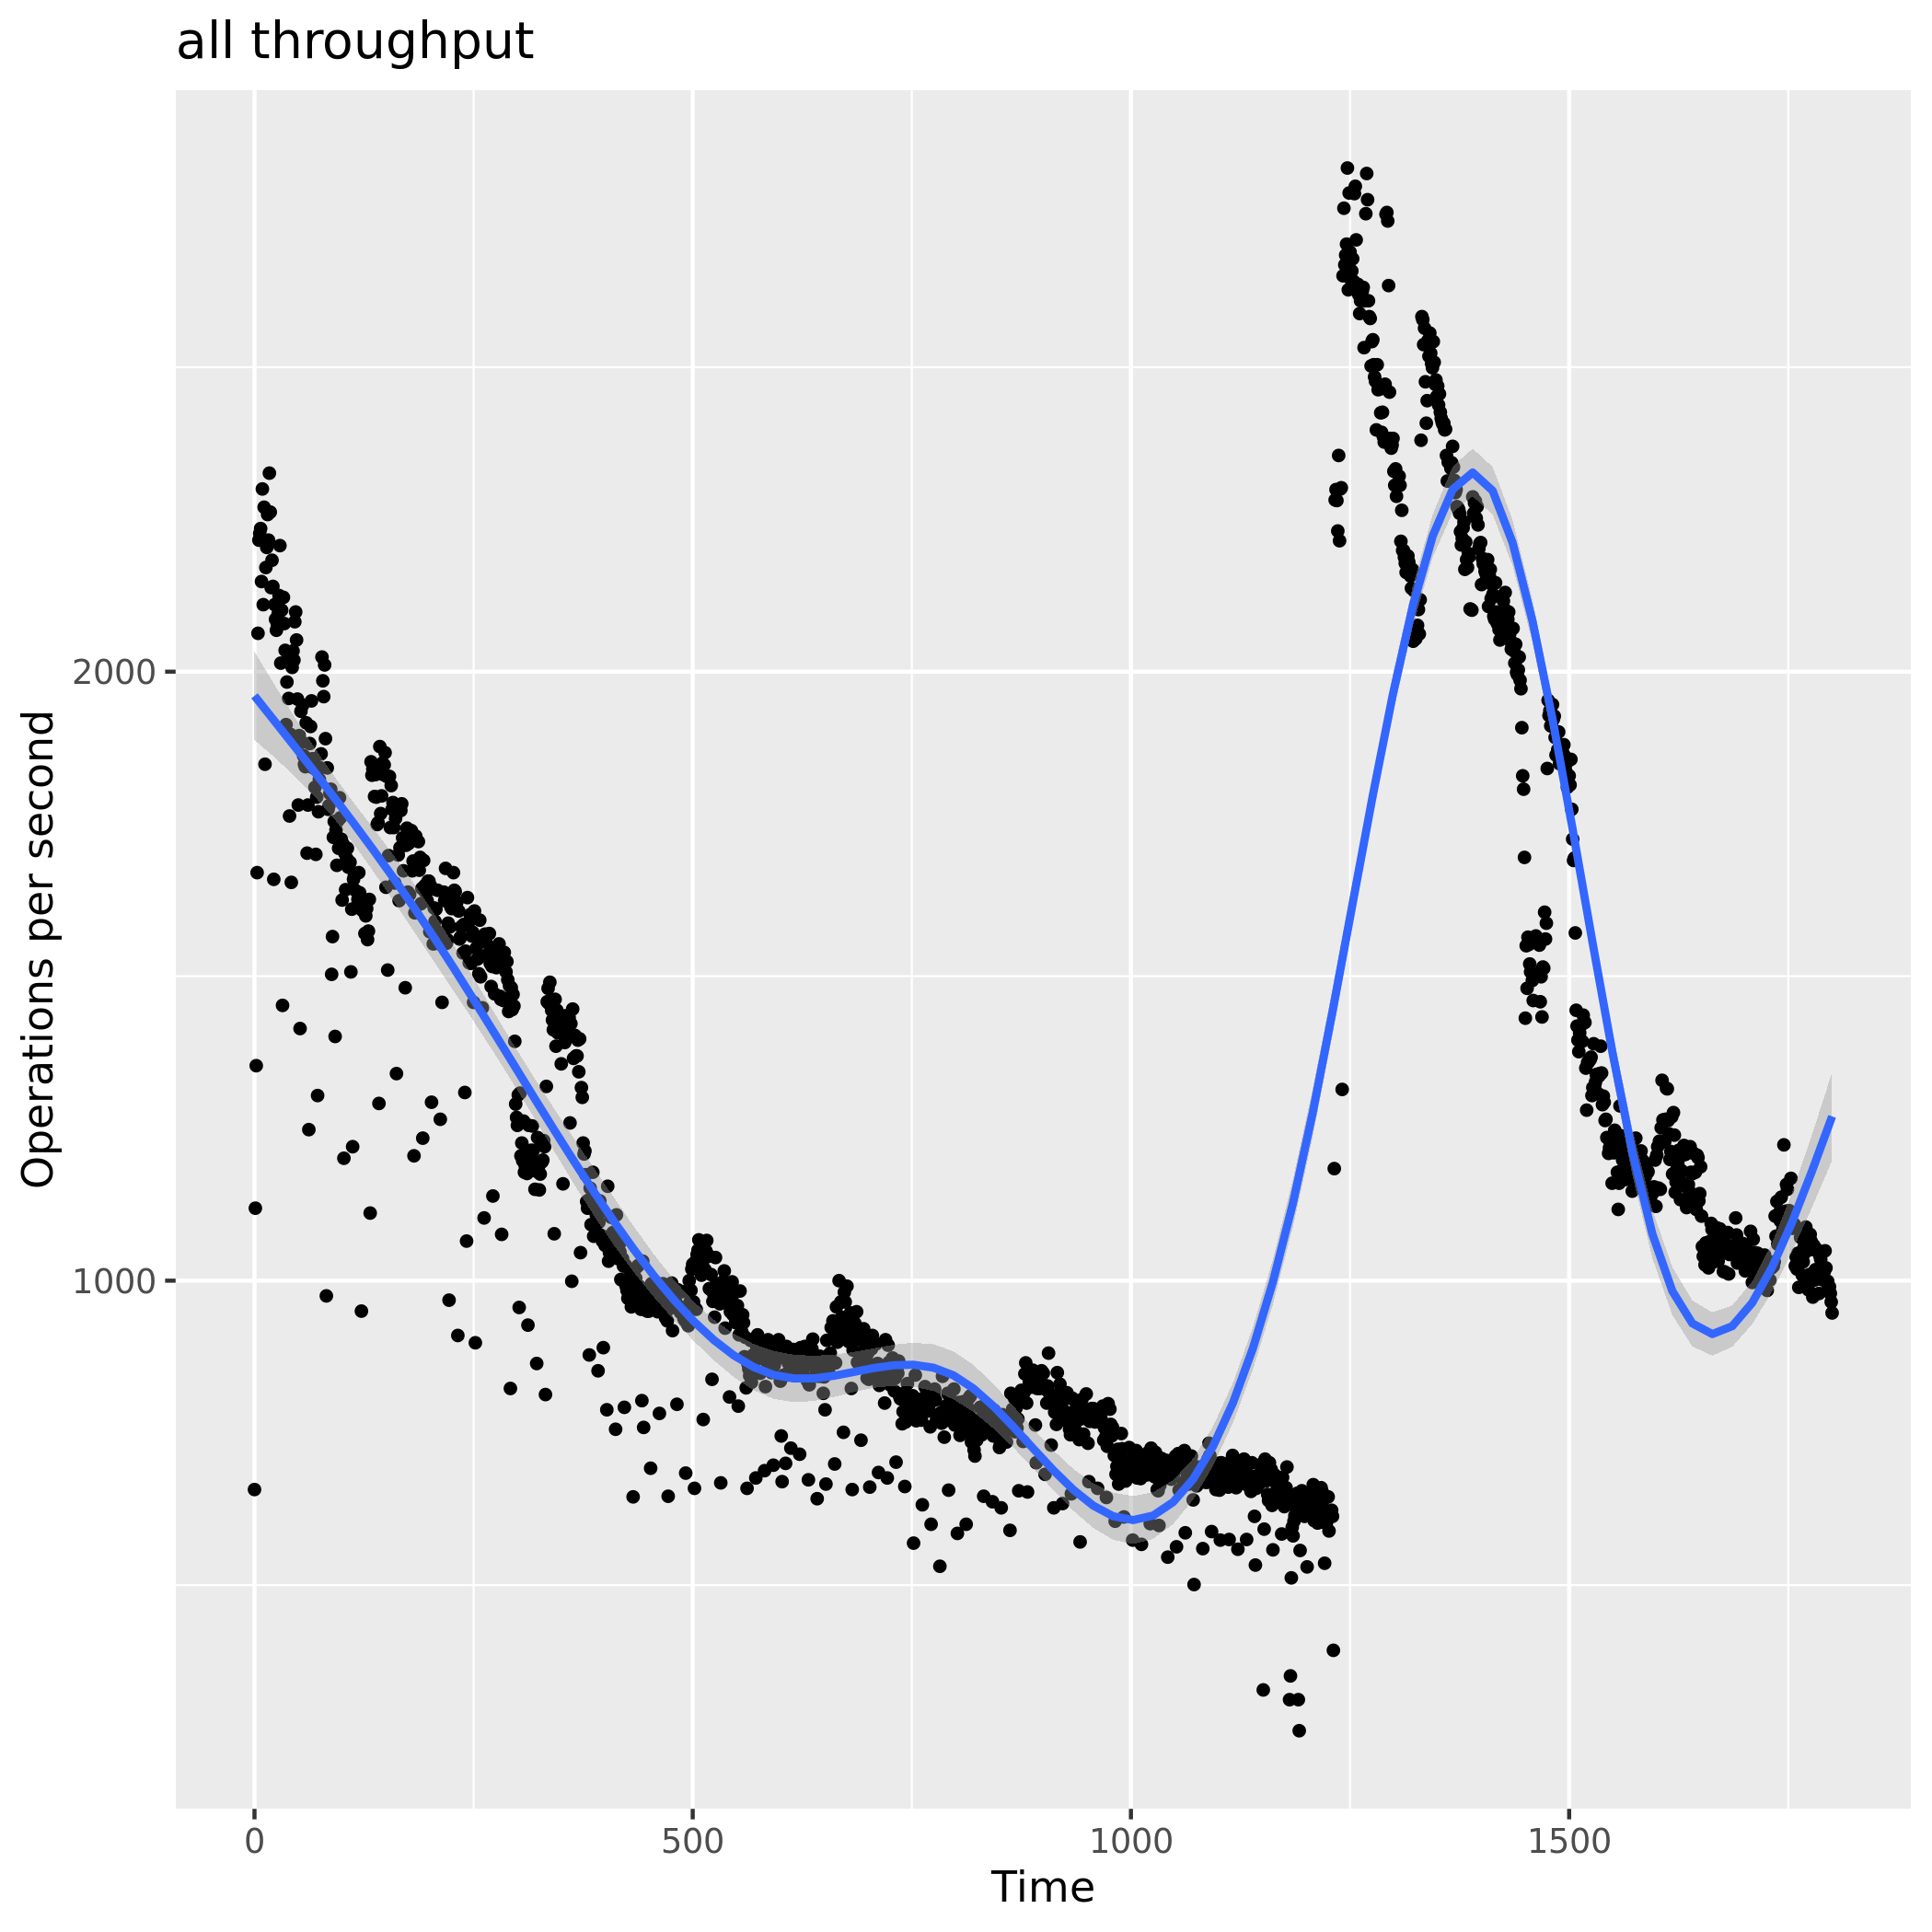
\includegraphics[width=0.5\textwidth]{RandomSlicing_Random_C1_write_heavy_throughput}
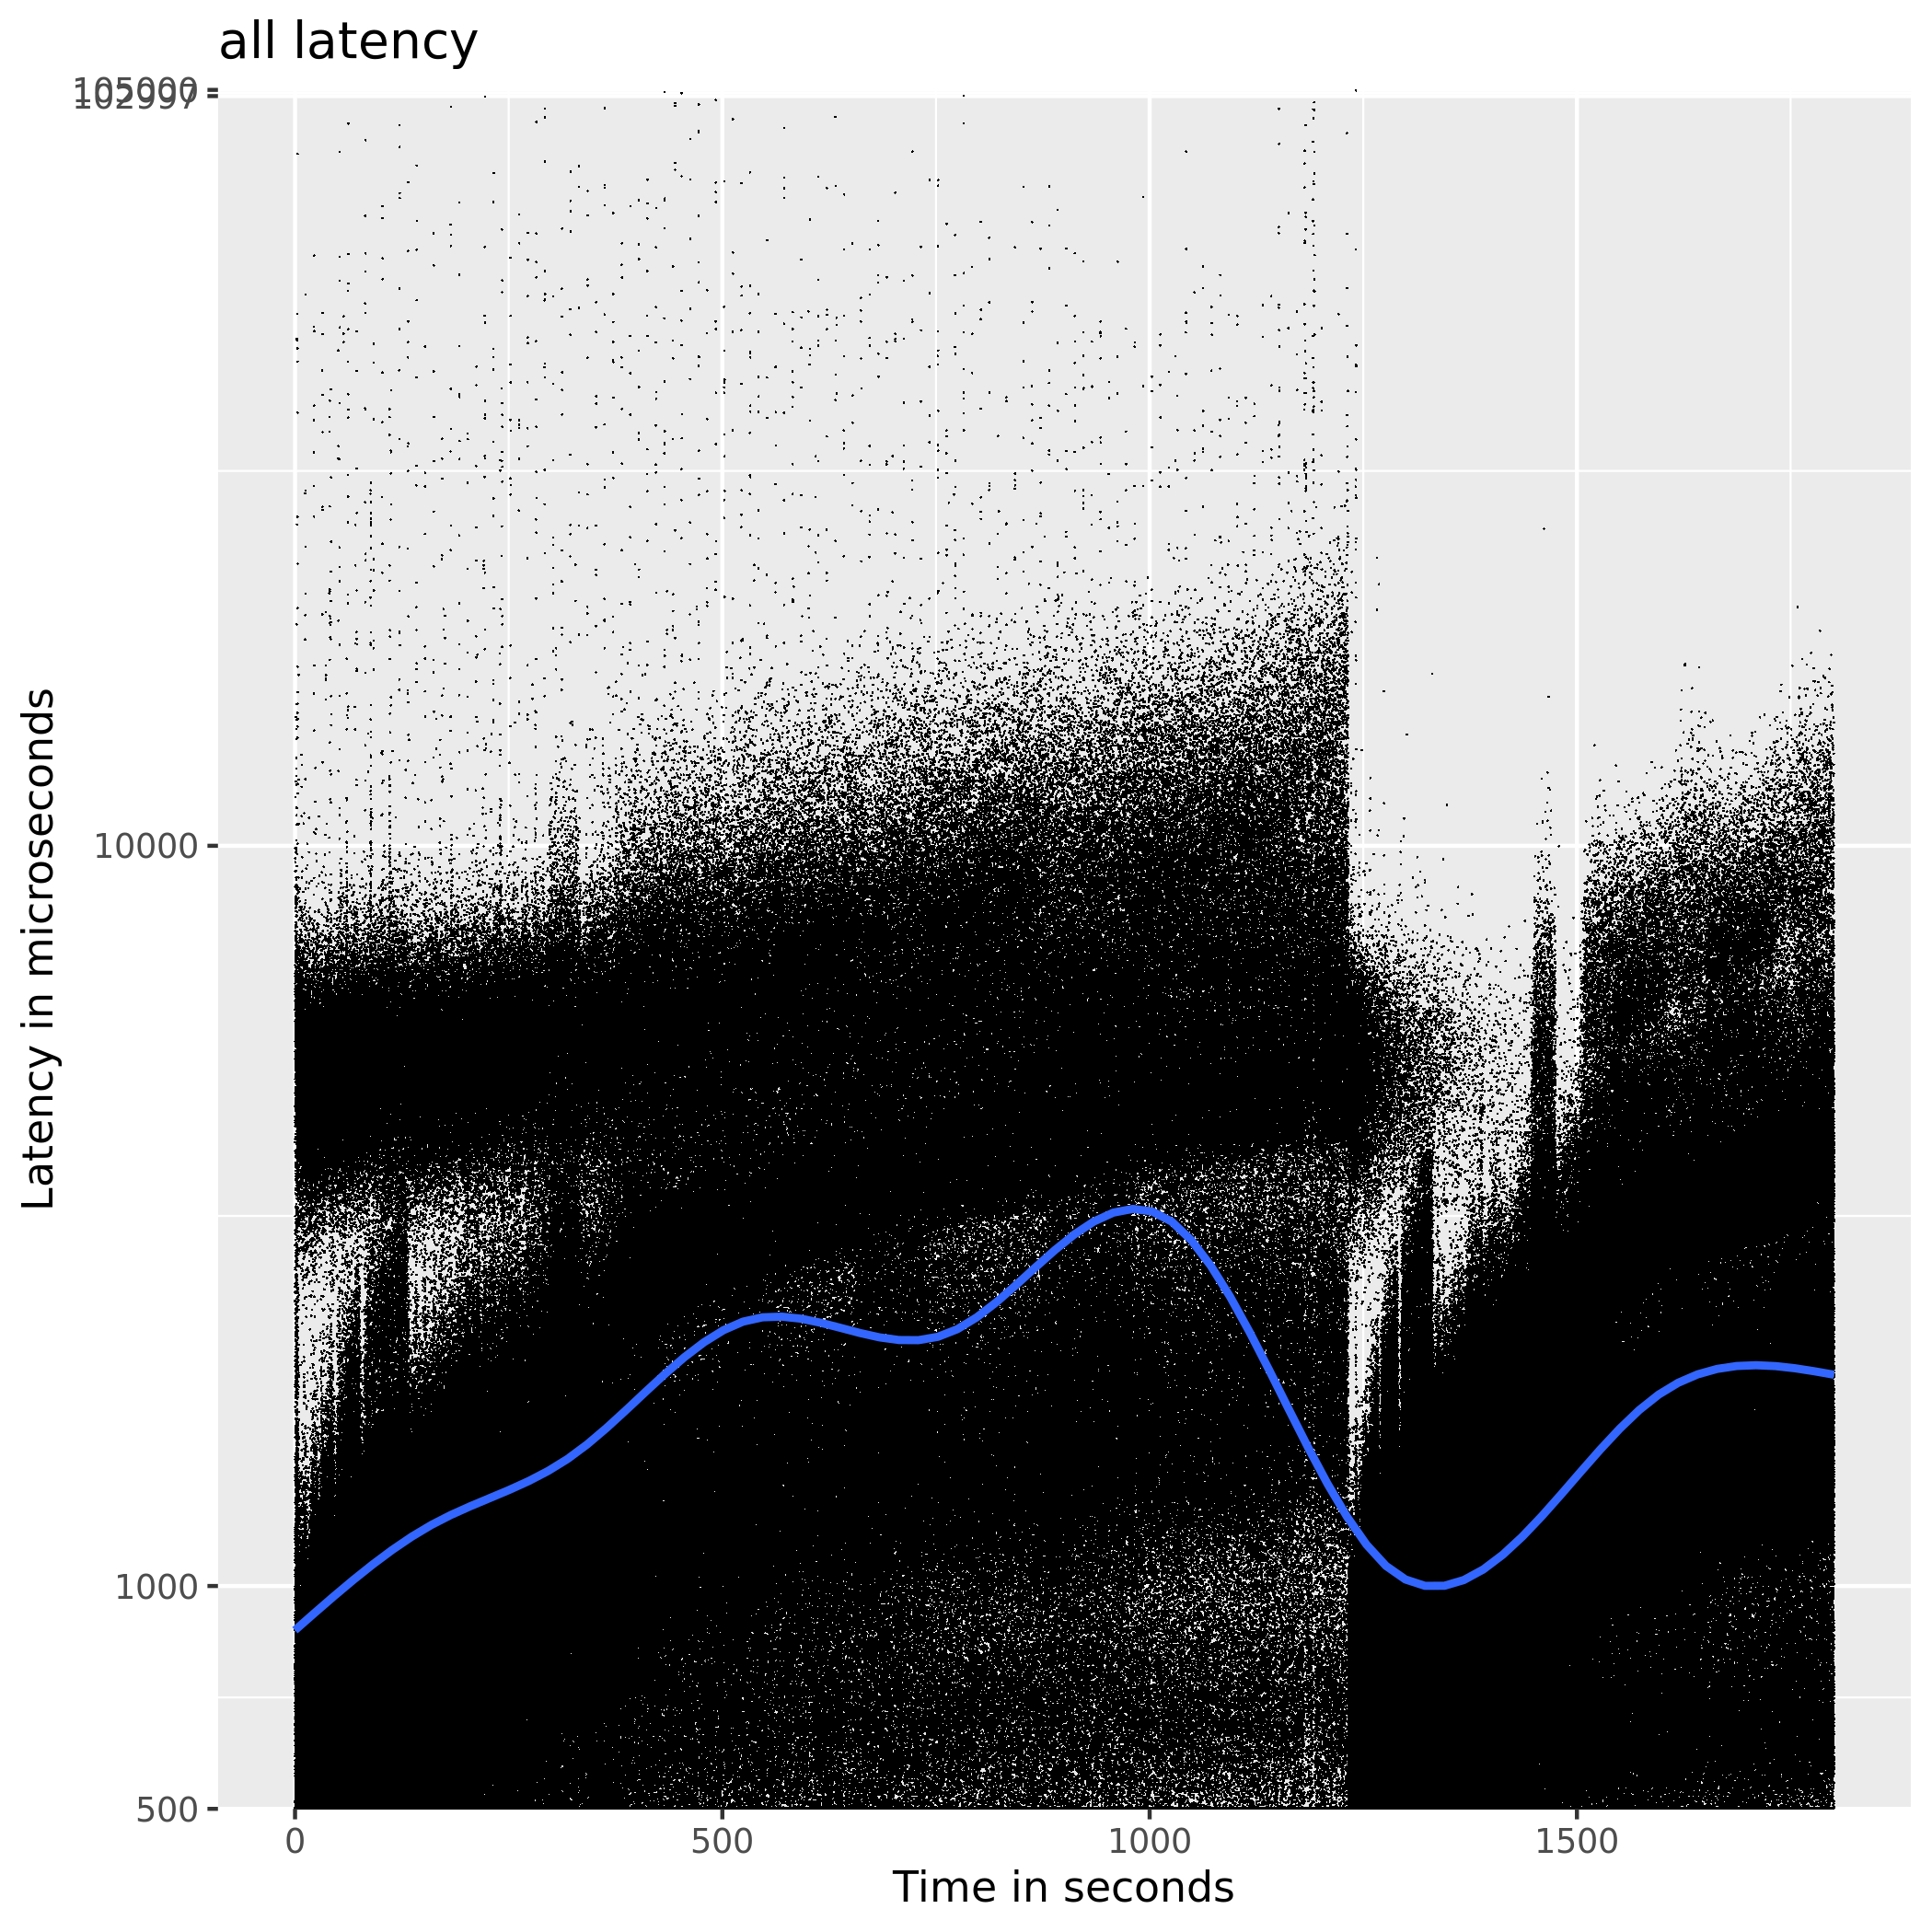
\includegraphics[width=0.5\textwidth]{RandomSlicing_Random_C1_write_heavy_latency}
\caption[\ac{RS} with Ramdom Replication Anomaly]{\ac{RS} with Ramdom Replication Anomaly. Even though the configuration is supposed to be static the throughput and latency plots show signs of a cluster change at 1300s.}
\label{fig:random_slicing_random_anomaly}
\end{figure}
These are signs that imply a cluster change and handoff started at that time according to all dynamic runs.
Assuming this is the case this run has to be excluded from the results.
There is a clear decline in performance when looking at configuration C2 with seven as the throughput starts at 750 operations per second and declines to 500 operations per second.
\begin{figure}
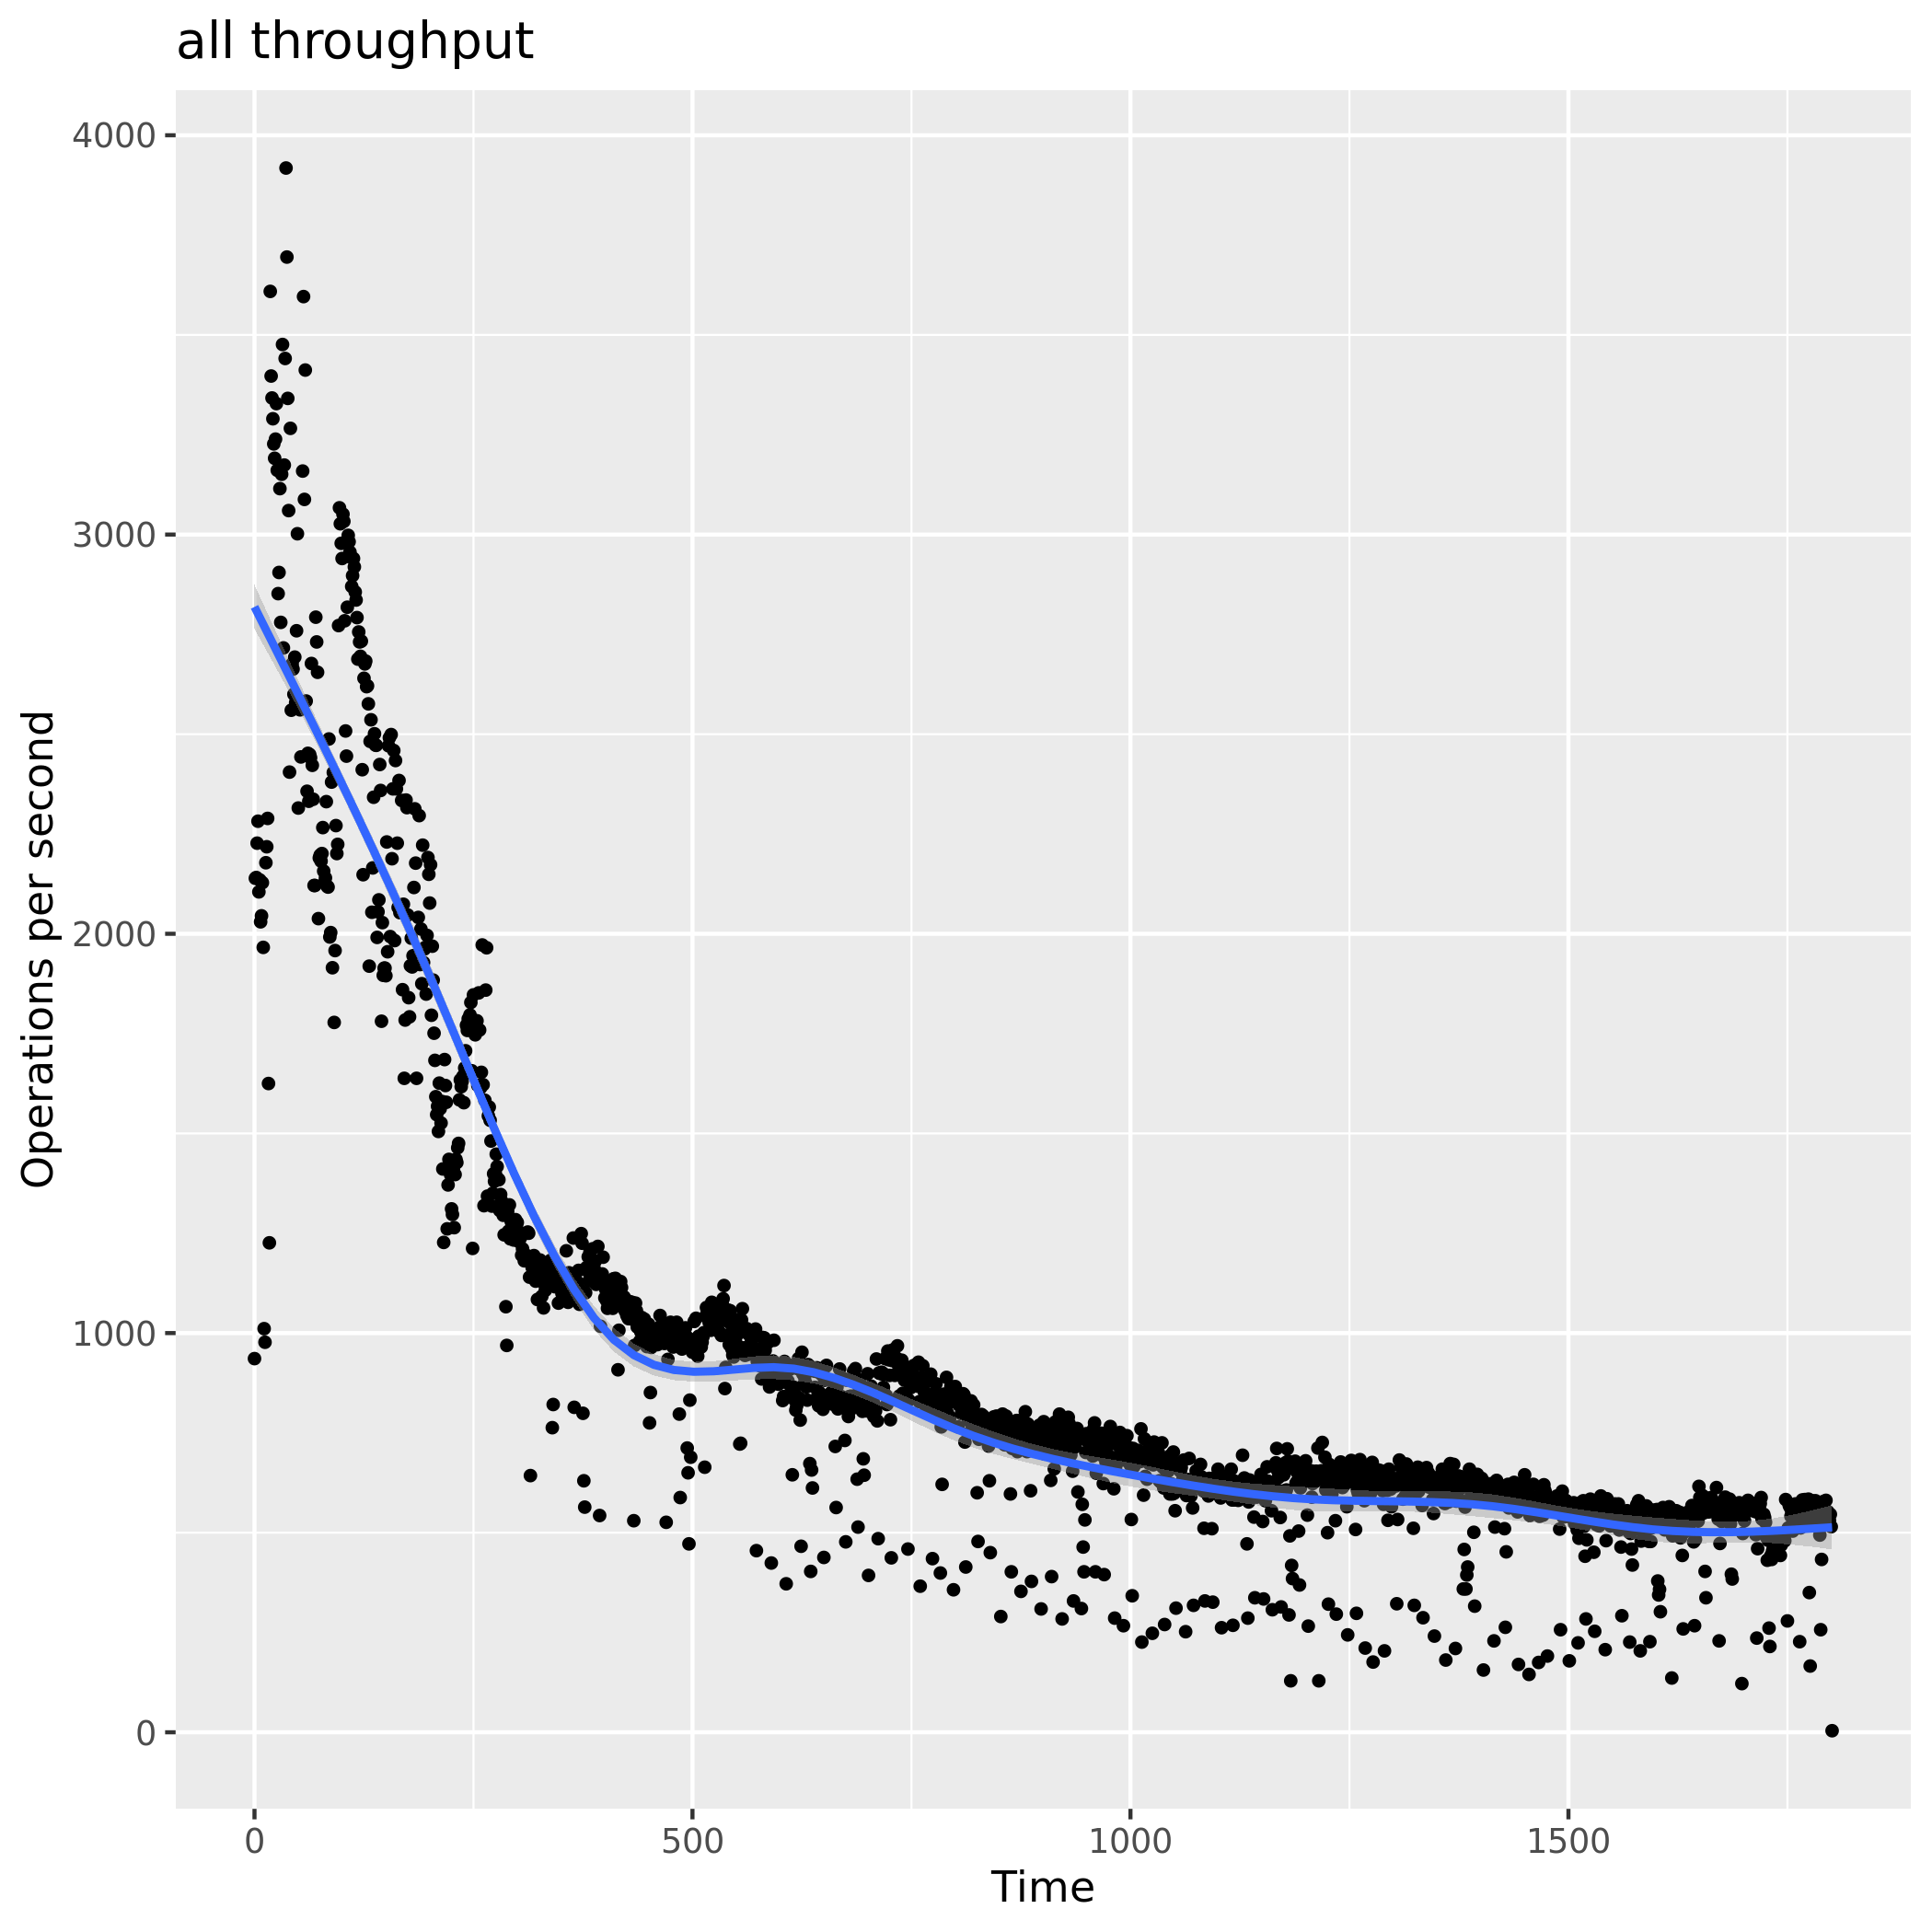
\includegraphics[width=0.5\textwidth]{RandomSlicing_Random_C0_write_heavy_throughput}
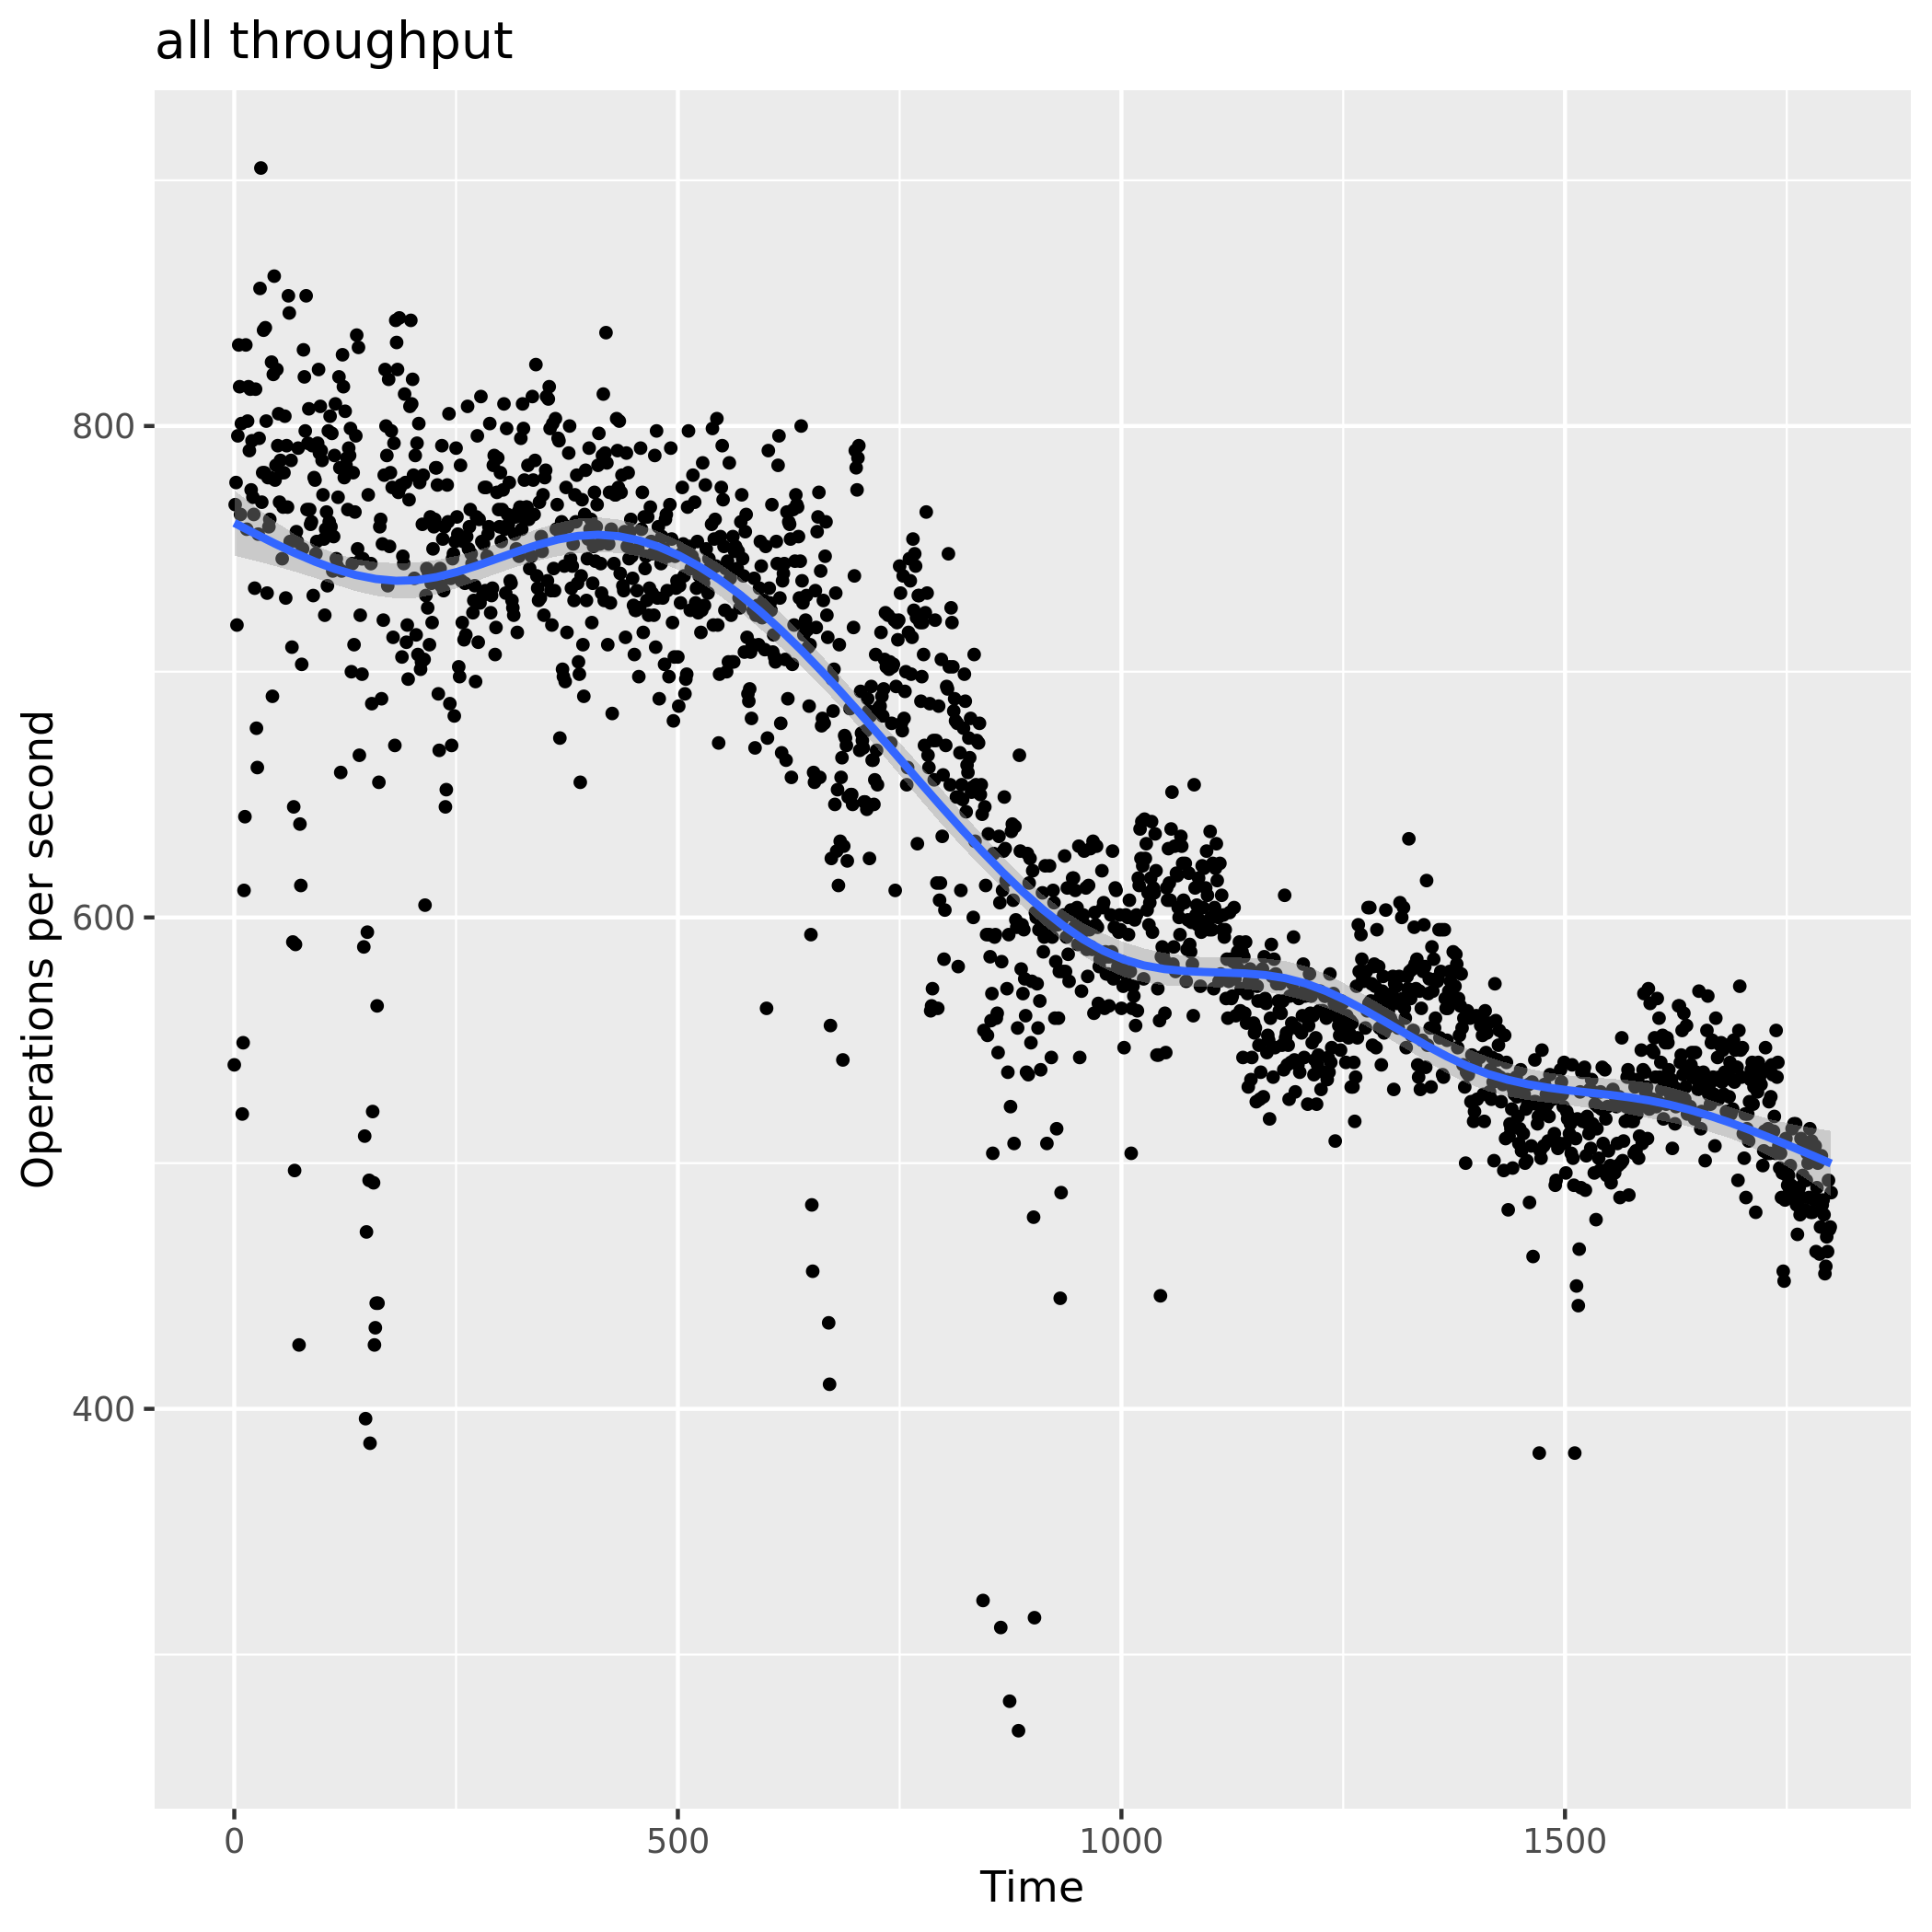
\includegraphics[width=0.5\textwidth]{RandomSlicing_Random_C2_write_heavy_throughput}
\caption[\ac{RS} with Ramdom Replication Throughput]{\ac{RS} with Ramdom Replication Throughput. Comparison of the throughput in C0 and C2.}
\label{fig:throughput_random_slicing_random}
\end{figure}

In the dynamic runs there seems to be a big difference in how the cluster changes are handled.
While the throughput seems to be quite similar in the sense that the second cluster change seems to have no big influence on the throughput the latency shows quite different images.
The latency plots of both workloads can be seen in \cref{fig:random_slicing_random_dynamic_latency}.
For the read-heavy workload there is an initial disruption at 600s and 1200s followed by a few smaller disruptions.
For the write-heavy workload there is a periodical occurrence of bigger disruptions starting at 600s and lasting up until 1000s.
These periodic disruptions do not show up as strongly after the second cluster change.
\begin{figure}
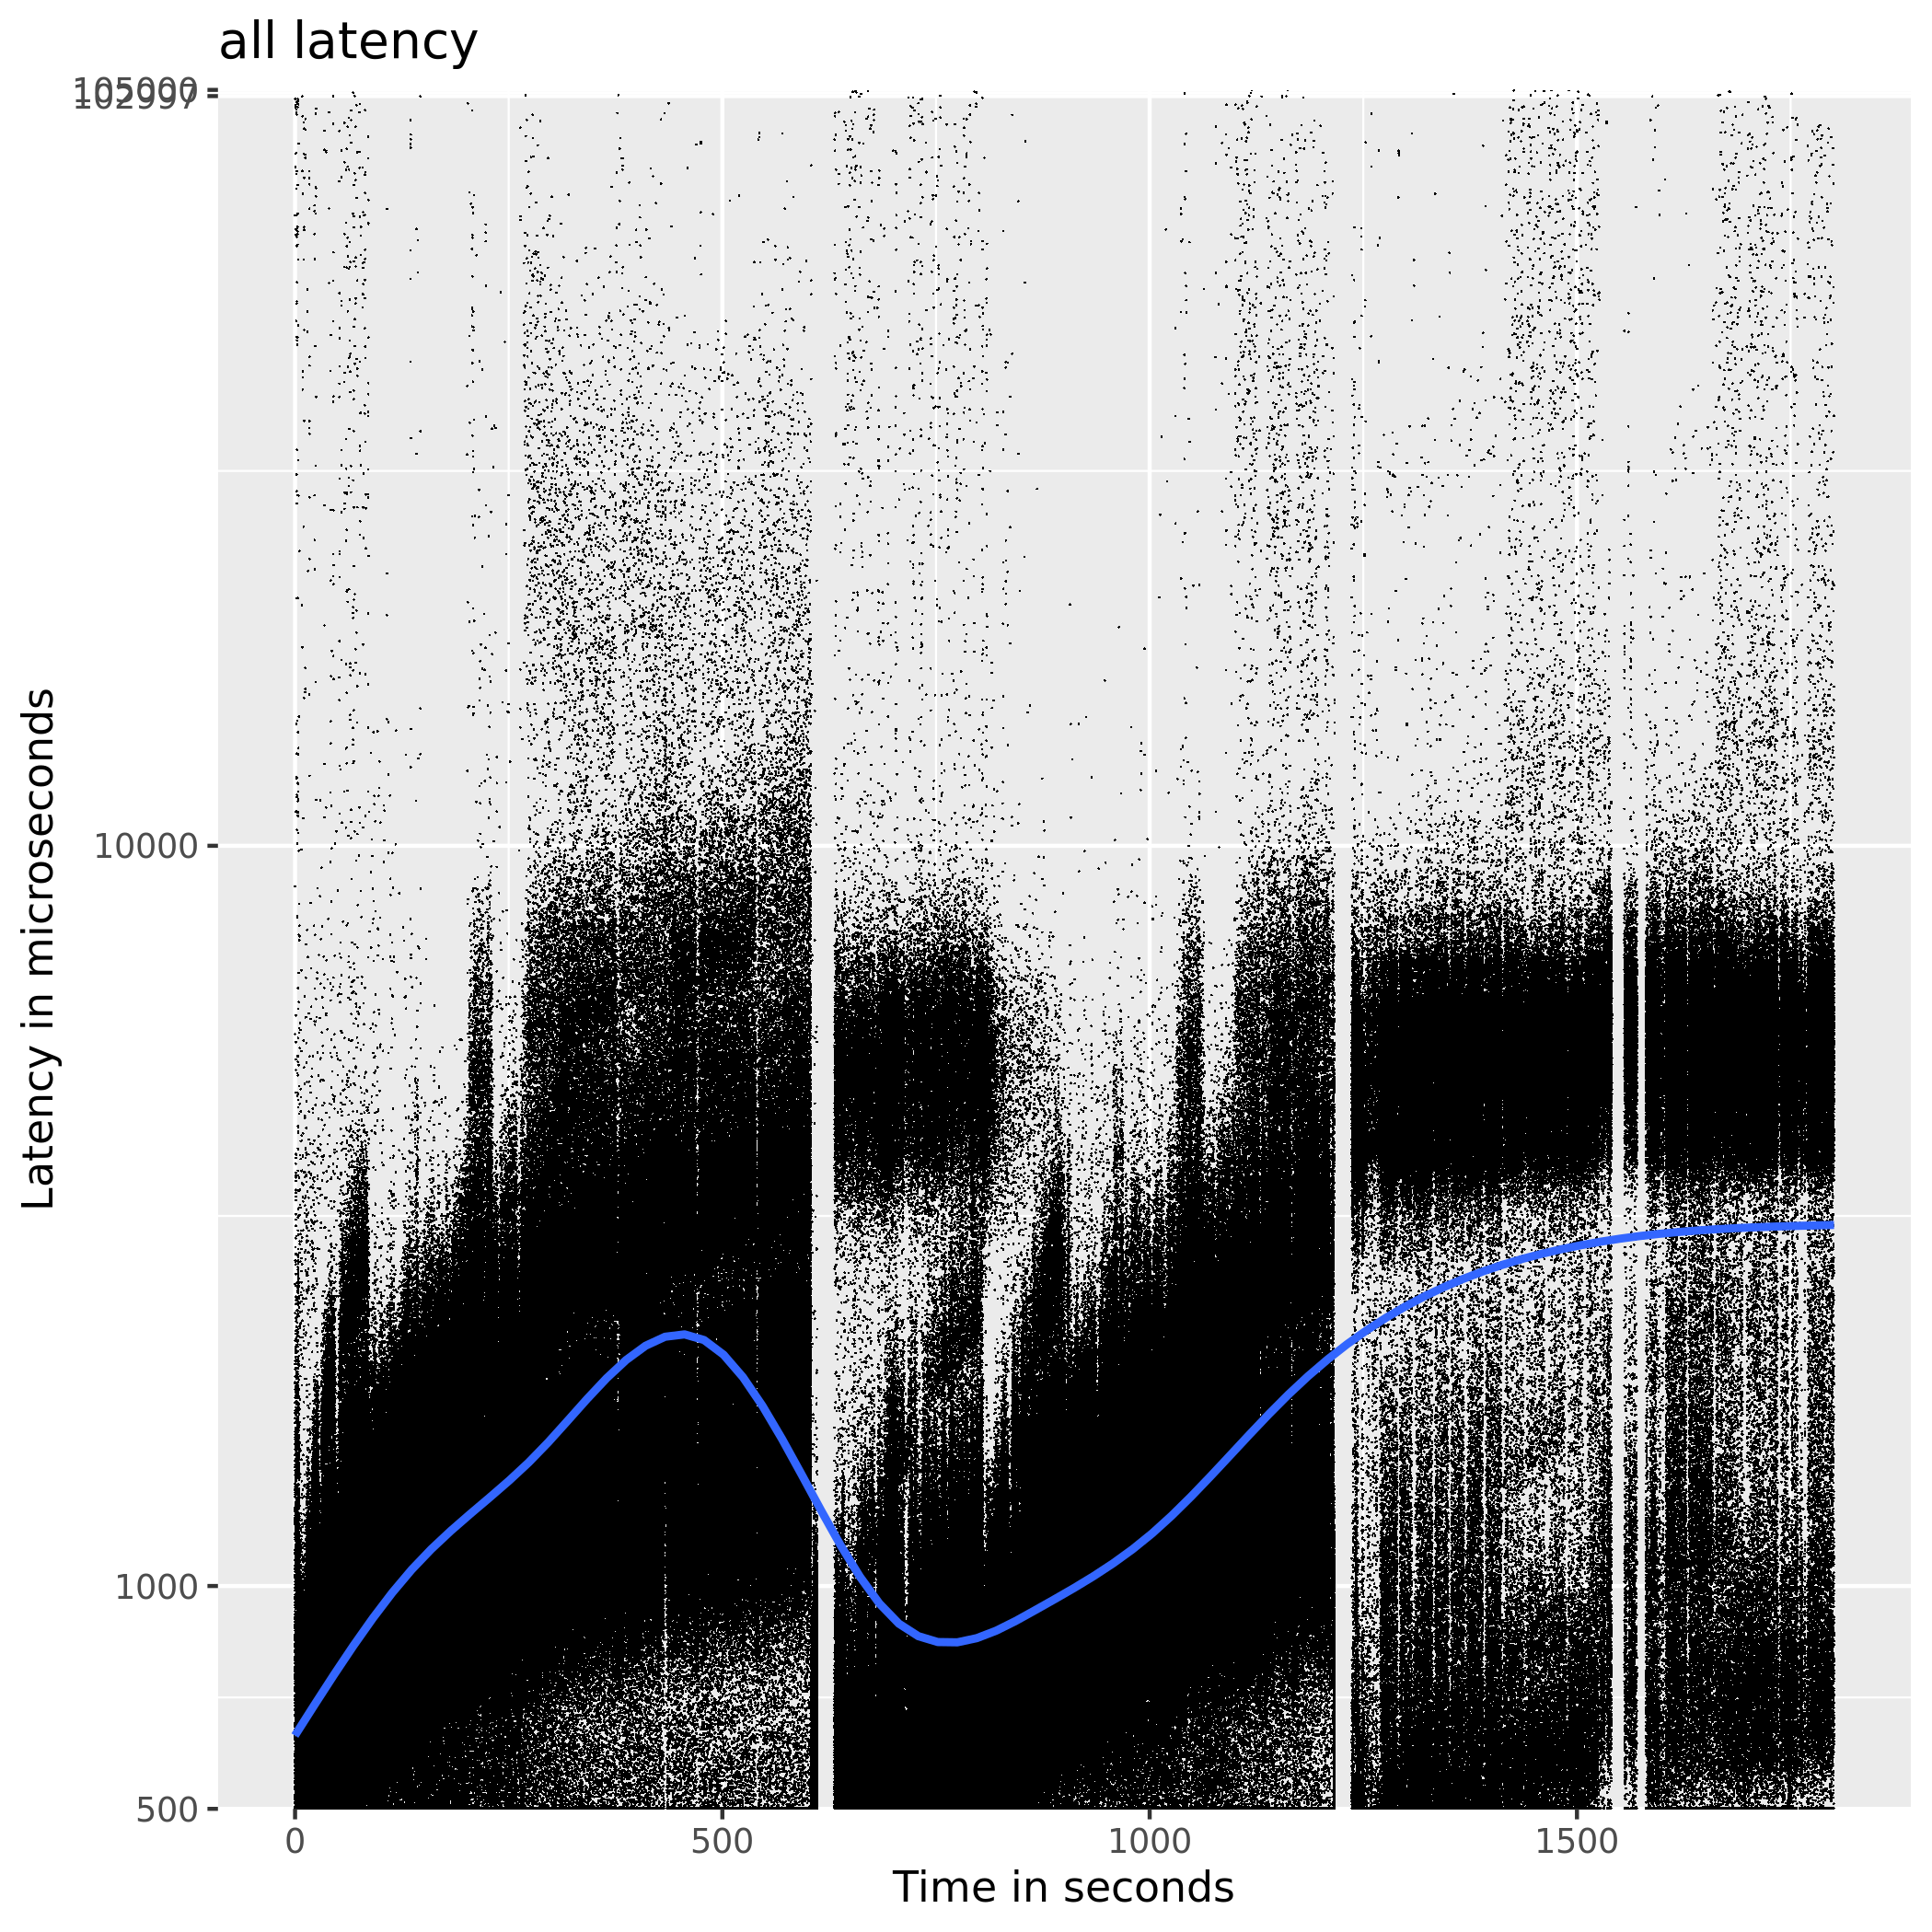
\includegraphics[width=0.5\textwidth]{RandomSlicing_Random_dynamic_read_heavy_latency}
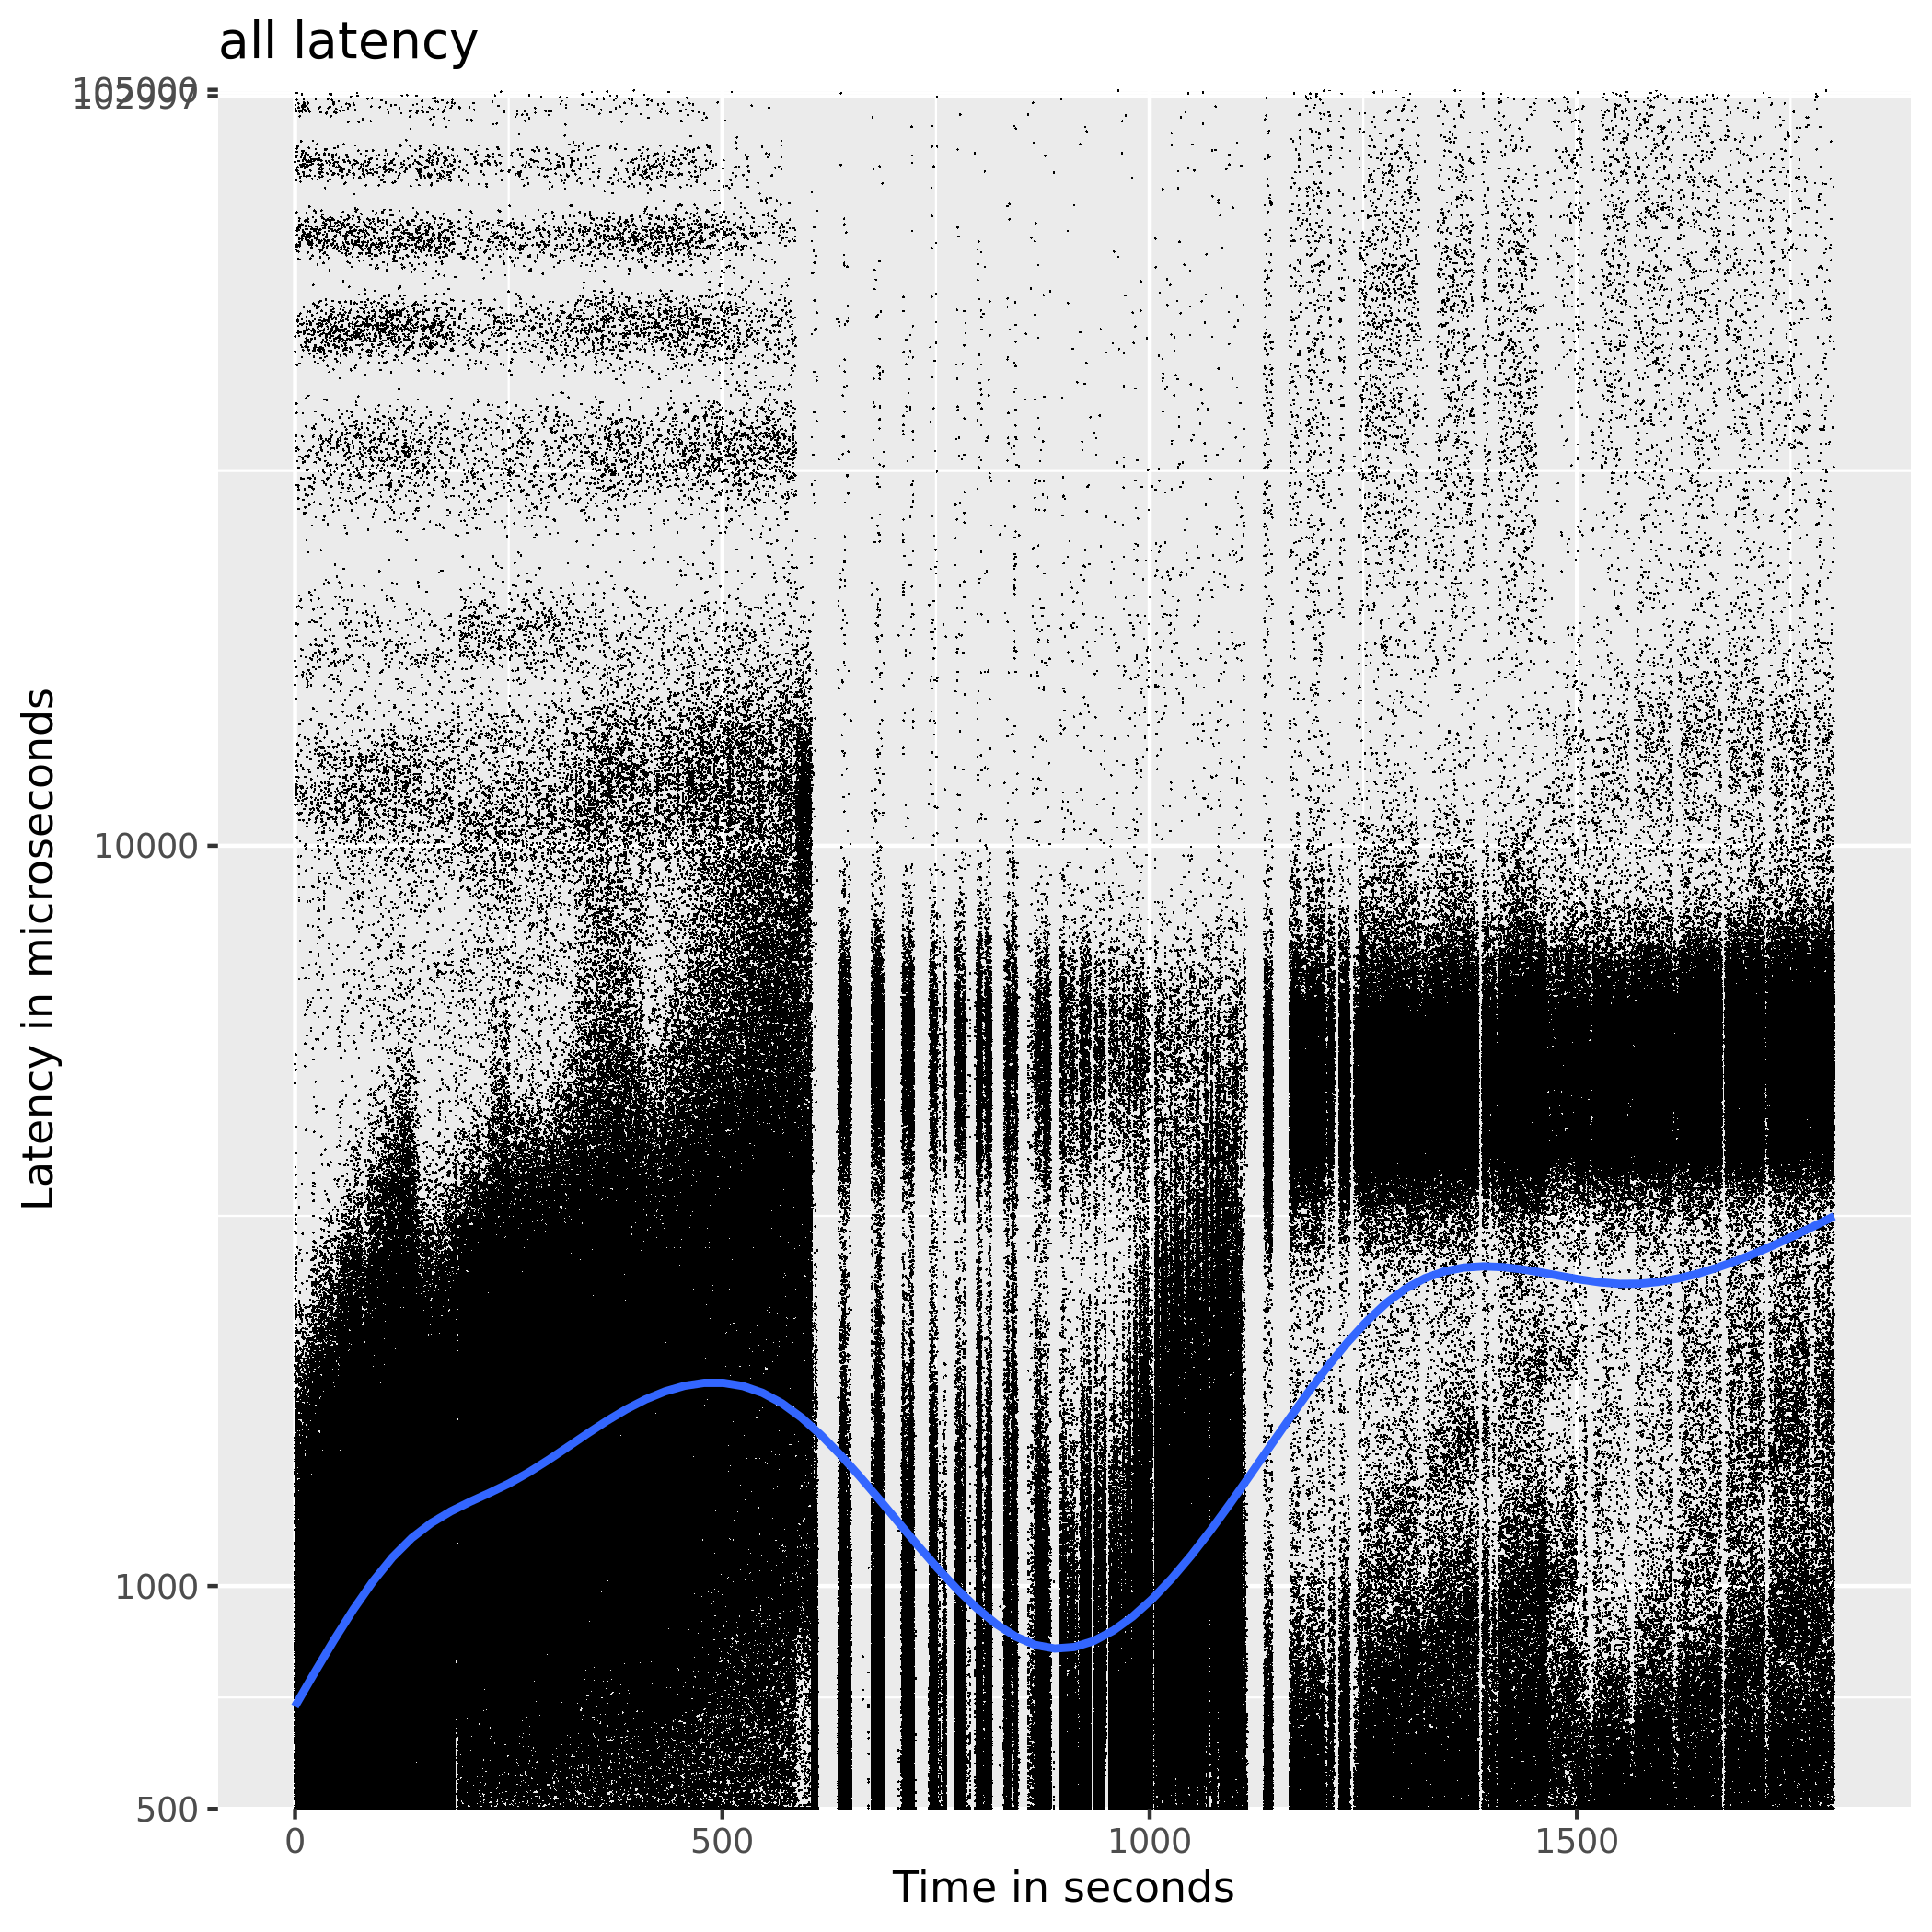
\includegraphics[width=0.5\textwidth]{RandomSlicing_Random_dynamic_write_heavy_latency}
\caption[\ac{RS} with Ramdom Replication Latency]{\ac{RS} with Ramdom Replication Latency. Comparison of the latency plots in the dynamic runs.}
\label{fig:random_slicing_random_dynamic_latency}
\end{figure}

Regarding the divergence from optimal load balance with \ac{RS} and Ring Jumping there is an absolute overall average divergence for key load of 0.022889616527552, for put load of 0.027008232485792, and for get load of 0.027078968645263.
Ignoring C0 with exactly three sections the highest divergence is measured in the dynamic configuration and the lowest is measured in C1.
This is quite intuitive as in C1 there are not many section and the sections are of a reasonable size while in the dynamic run the keys are potentially to the wrong node initially and will only be balanced after the repair operations are started for each key.

\subsection{Random Slicing Rotation}
The Ring Rotation \ac{RPS} implementation shows a lot of problems in the evaluation.
Apart from C0 and C1 every run with other configurations was far off any expected result or could not even be finished.
In C0 the throughput starts at about 3000 operations per second, steeply decreases to 1000 operations per second at 450s and from there slowly decreases to 500 operations per second.
In C1 the throughput starts at about 2100 operations per second, steeply decreases to 1000 operations per second at 500s and from there slowly decreases to 500 operations per second.
The first problematic run is the write-heavy run in C2, as the throughput stays at single-digit operations per second over the complete run, which can be seen in \cref{fig:random_slicing_rotation_throughput}.
\begin{figure}
\center
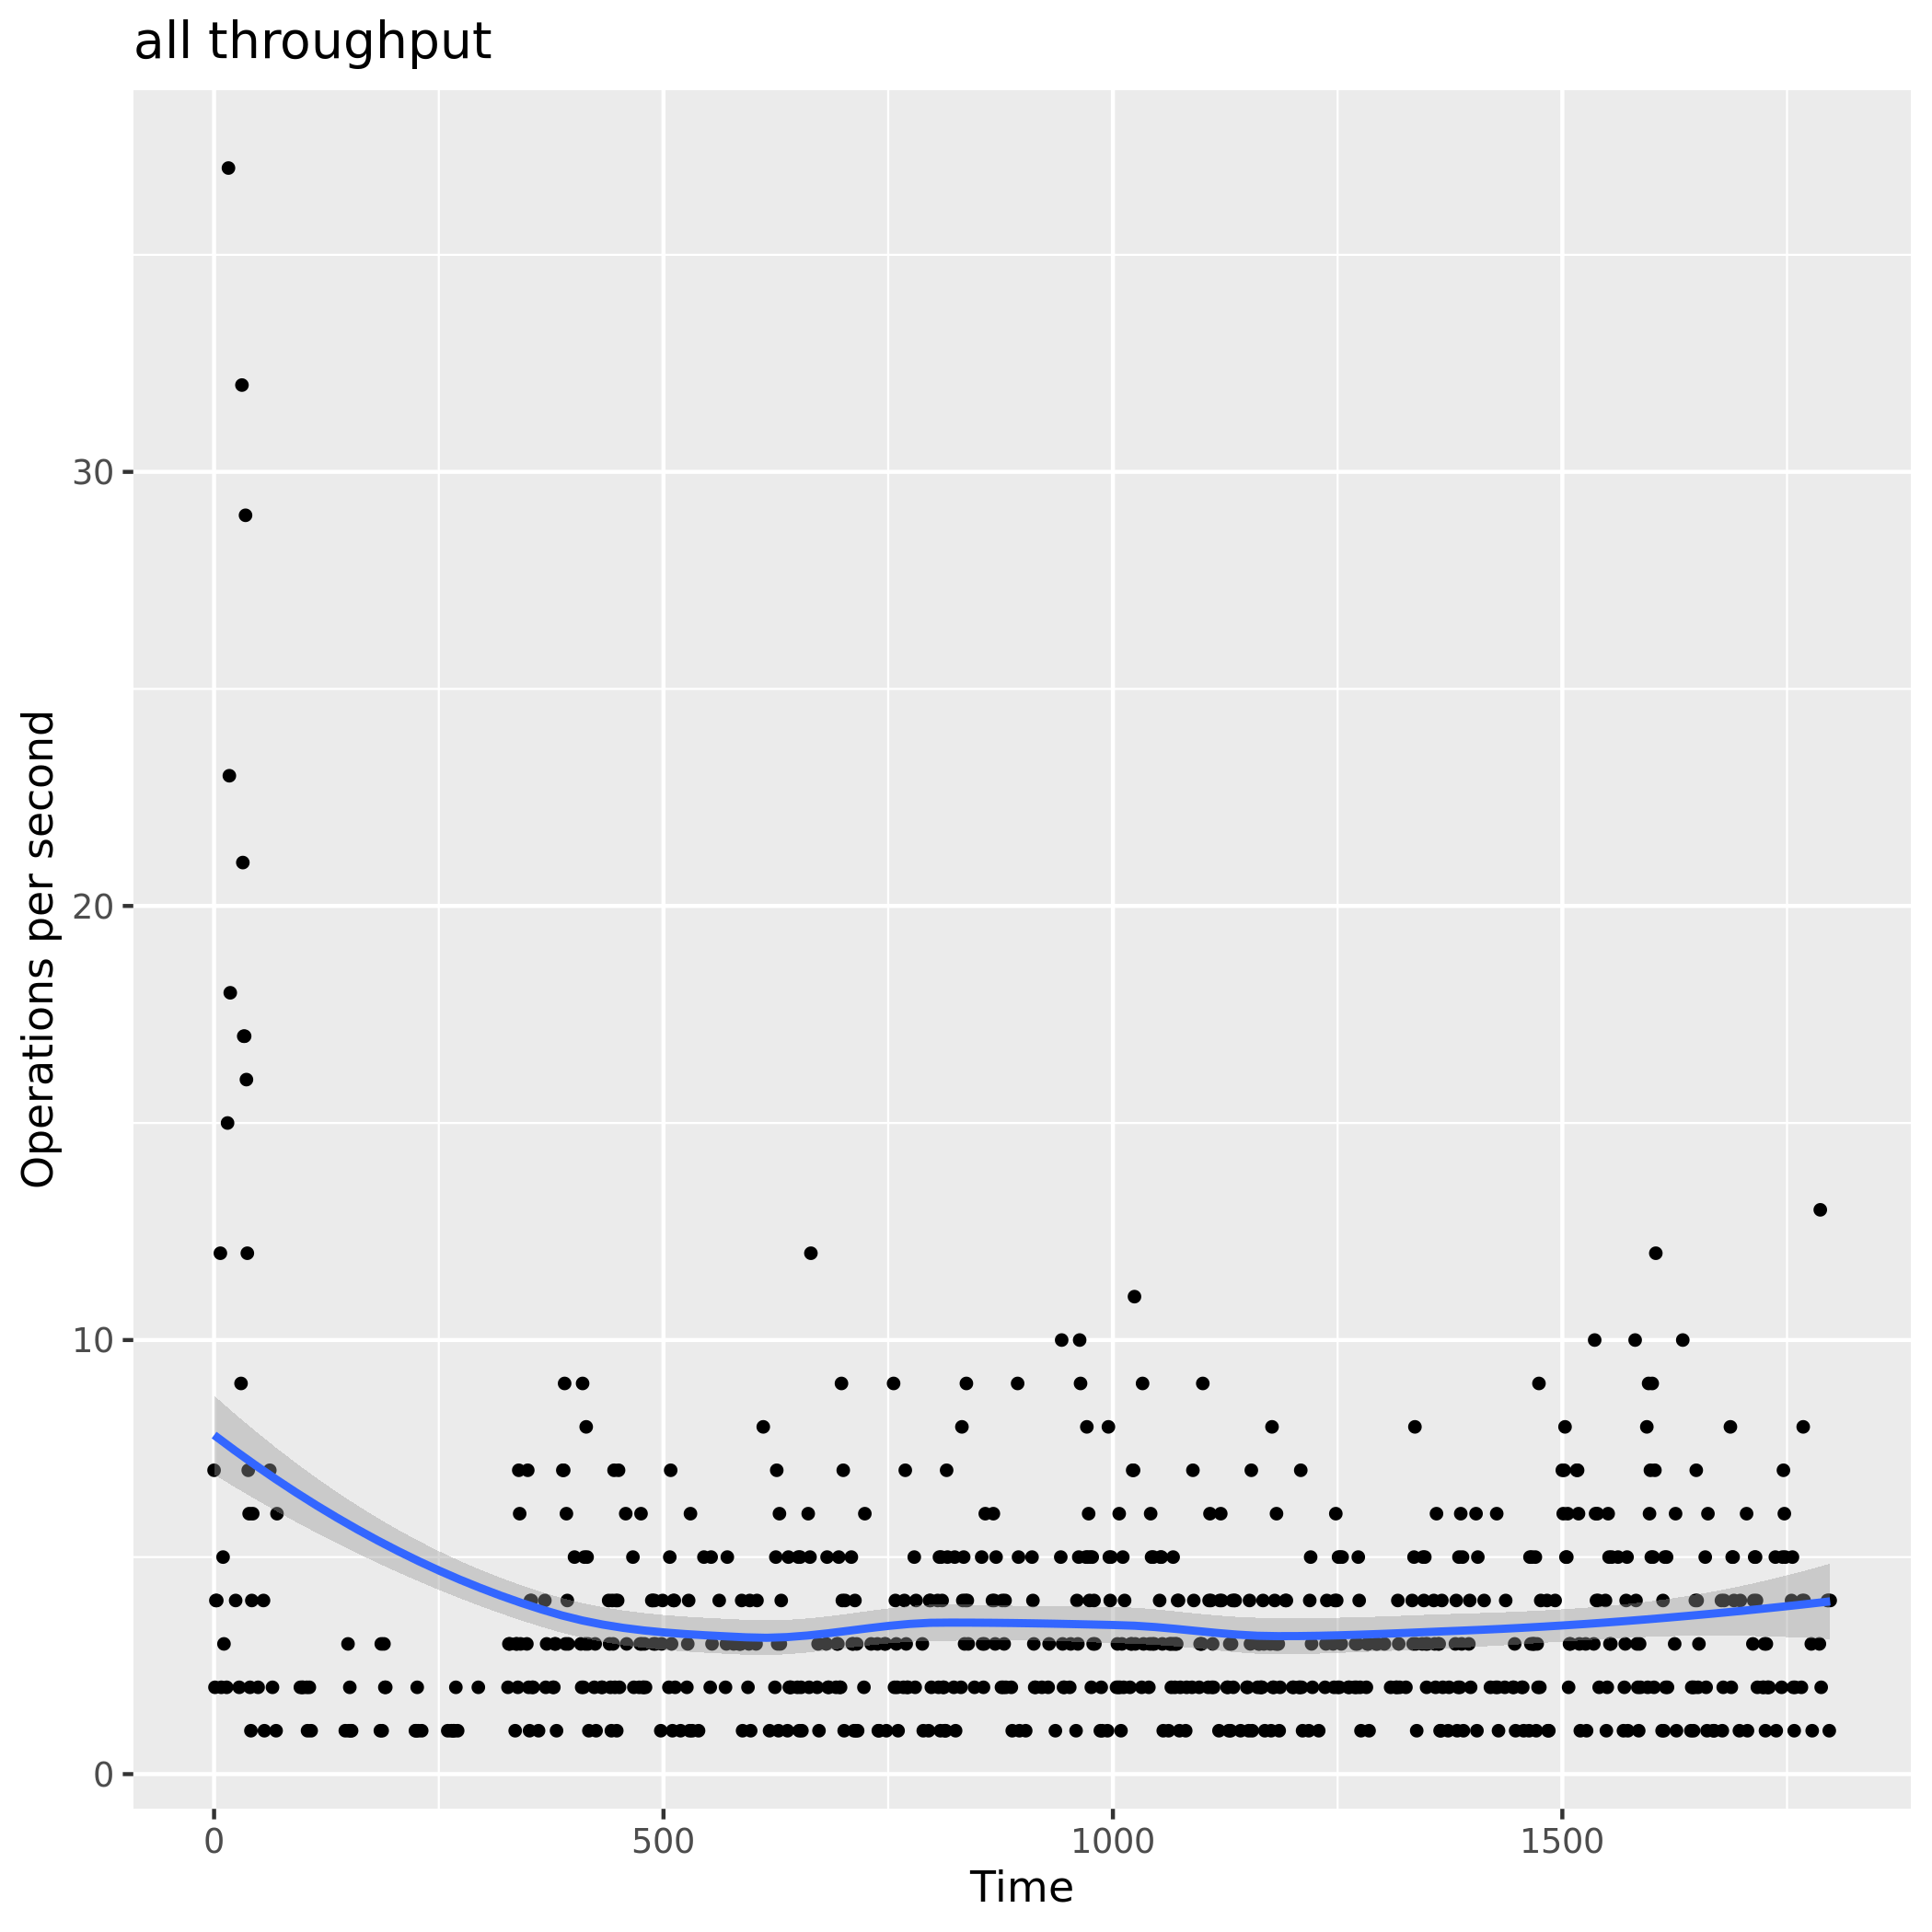
\includegraphics[width=0.5\textwidth]{RandomSlicing_Rotation_C2_write_heavy_throughput}
\caption[Low Throughput with Ring Rotation]{Low Throughput with Ring Rotation}
\label{fig:random_slicing_rotation_throughput}
\end{figure}
Trying to rerun this configuration to confirm the result showed a potential memory leak that seems to be occur more frequently with a higher number of sections.

This memory leak became quite apparent as even after multiple restarts the benchmark runs could not be finished in the dynamic configurations as the memory leak caused the run to crash each time.
An assertion on the overall load balance is also impossible through this.


\subsection{Comparison}
In this section we compare the evaluation results of the different \ac{RCL} configurations and focus on how our hypotheses are supported or contradicted.
As there is not enough data and configurations to properly test the hypotheses we use the available evaluation data to quantitatively compare the different approaches.

\subsubsection{Hypothesis 1}
Hypothesis 1 claims that \ac{RS} has the best load balance when Random Replication is used as the replication placement strategy.
As Random Replication produces the better overall load balance and also has a lower absolute divergence for every configuration and parameter than Ring Rotation and Ring Jumping we can assume Hypothesis 1 as plausible.

\subsubsection{Hypothesis 2}
Hypothesis 2 claims that \ac{RS} has the highest throughput when Random Replication is used as the replication placement strategy.
Apart from the Ring Rotation strategy, which shows a strong decline in throughput with a growing number of ring sections, the throughput plots have the same characteristics for the different \acp{RPS}.
They show that the throughput starts at about the same rate, decreases to similar values at equal times and also ends at the same rate.
Therefore there is no argument for or against the hypothesis with the available data and as is shown with Ring Rotation it may be a matter of scalability of the strategies.

\subsubsection{Hypothesis 3}
Hypothesis 3 claims that the load divergence of \ac{RS} with the best replication placement strategy is at most 10\% higher than with Consistent Hashing.
We use the results of \ac{RS} with Random Replication as this yielded the best balancing properties and a high throughput.
While the divergence of load concerning unique keys with \ac{RS} is nearly 6 times the one with Consistent Hashing, the divergence concerning operations is only slightly more than 10\% higher.
However, this clearly shows strong arguments against the presented hypothesis for the current integration of \ac{RS} with \ac{RCL}.
As a side remark it is interesting to see that \ac{RS} with Consistent Hashing achieves a way better load balance in configuration C2 than Consistent Hashing and it will be interesting to see how both systems scale for more nodes.

\subsubsection{Hypothesis 4}
Hypothesis 4 claims that \ac{RS} generates a throughput that is nearly as good as Consistent Hashing in a static cluster configuration.
As there is no clear difference in throughput we choose Random Replication as the replication placement strategy.
As can be seen in the side-to-side comparison in \cref{fig:throughput_comparison} there is no significant difference between Consistent Hashing and \ac{RS} in any static configuration.
\begin{figure}
\begin{subfigure}{0.5\textwidth}
	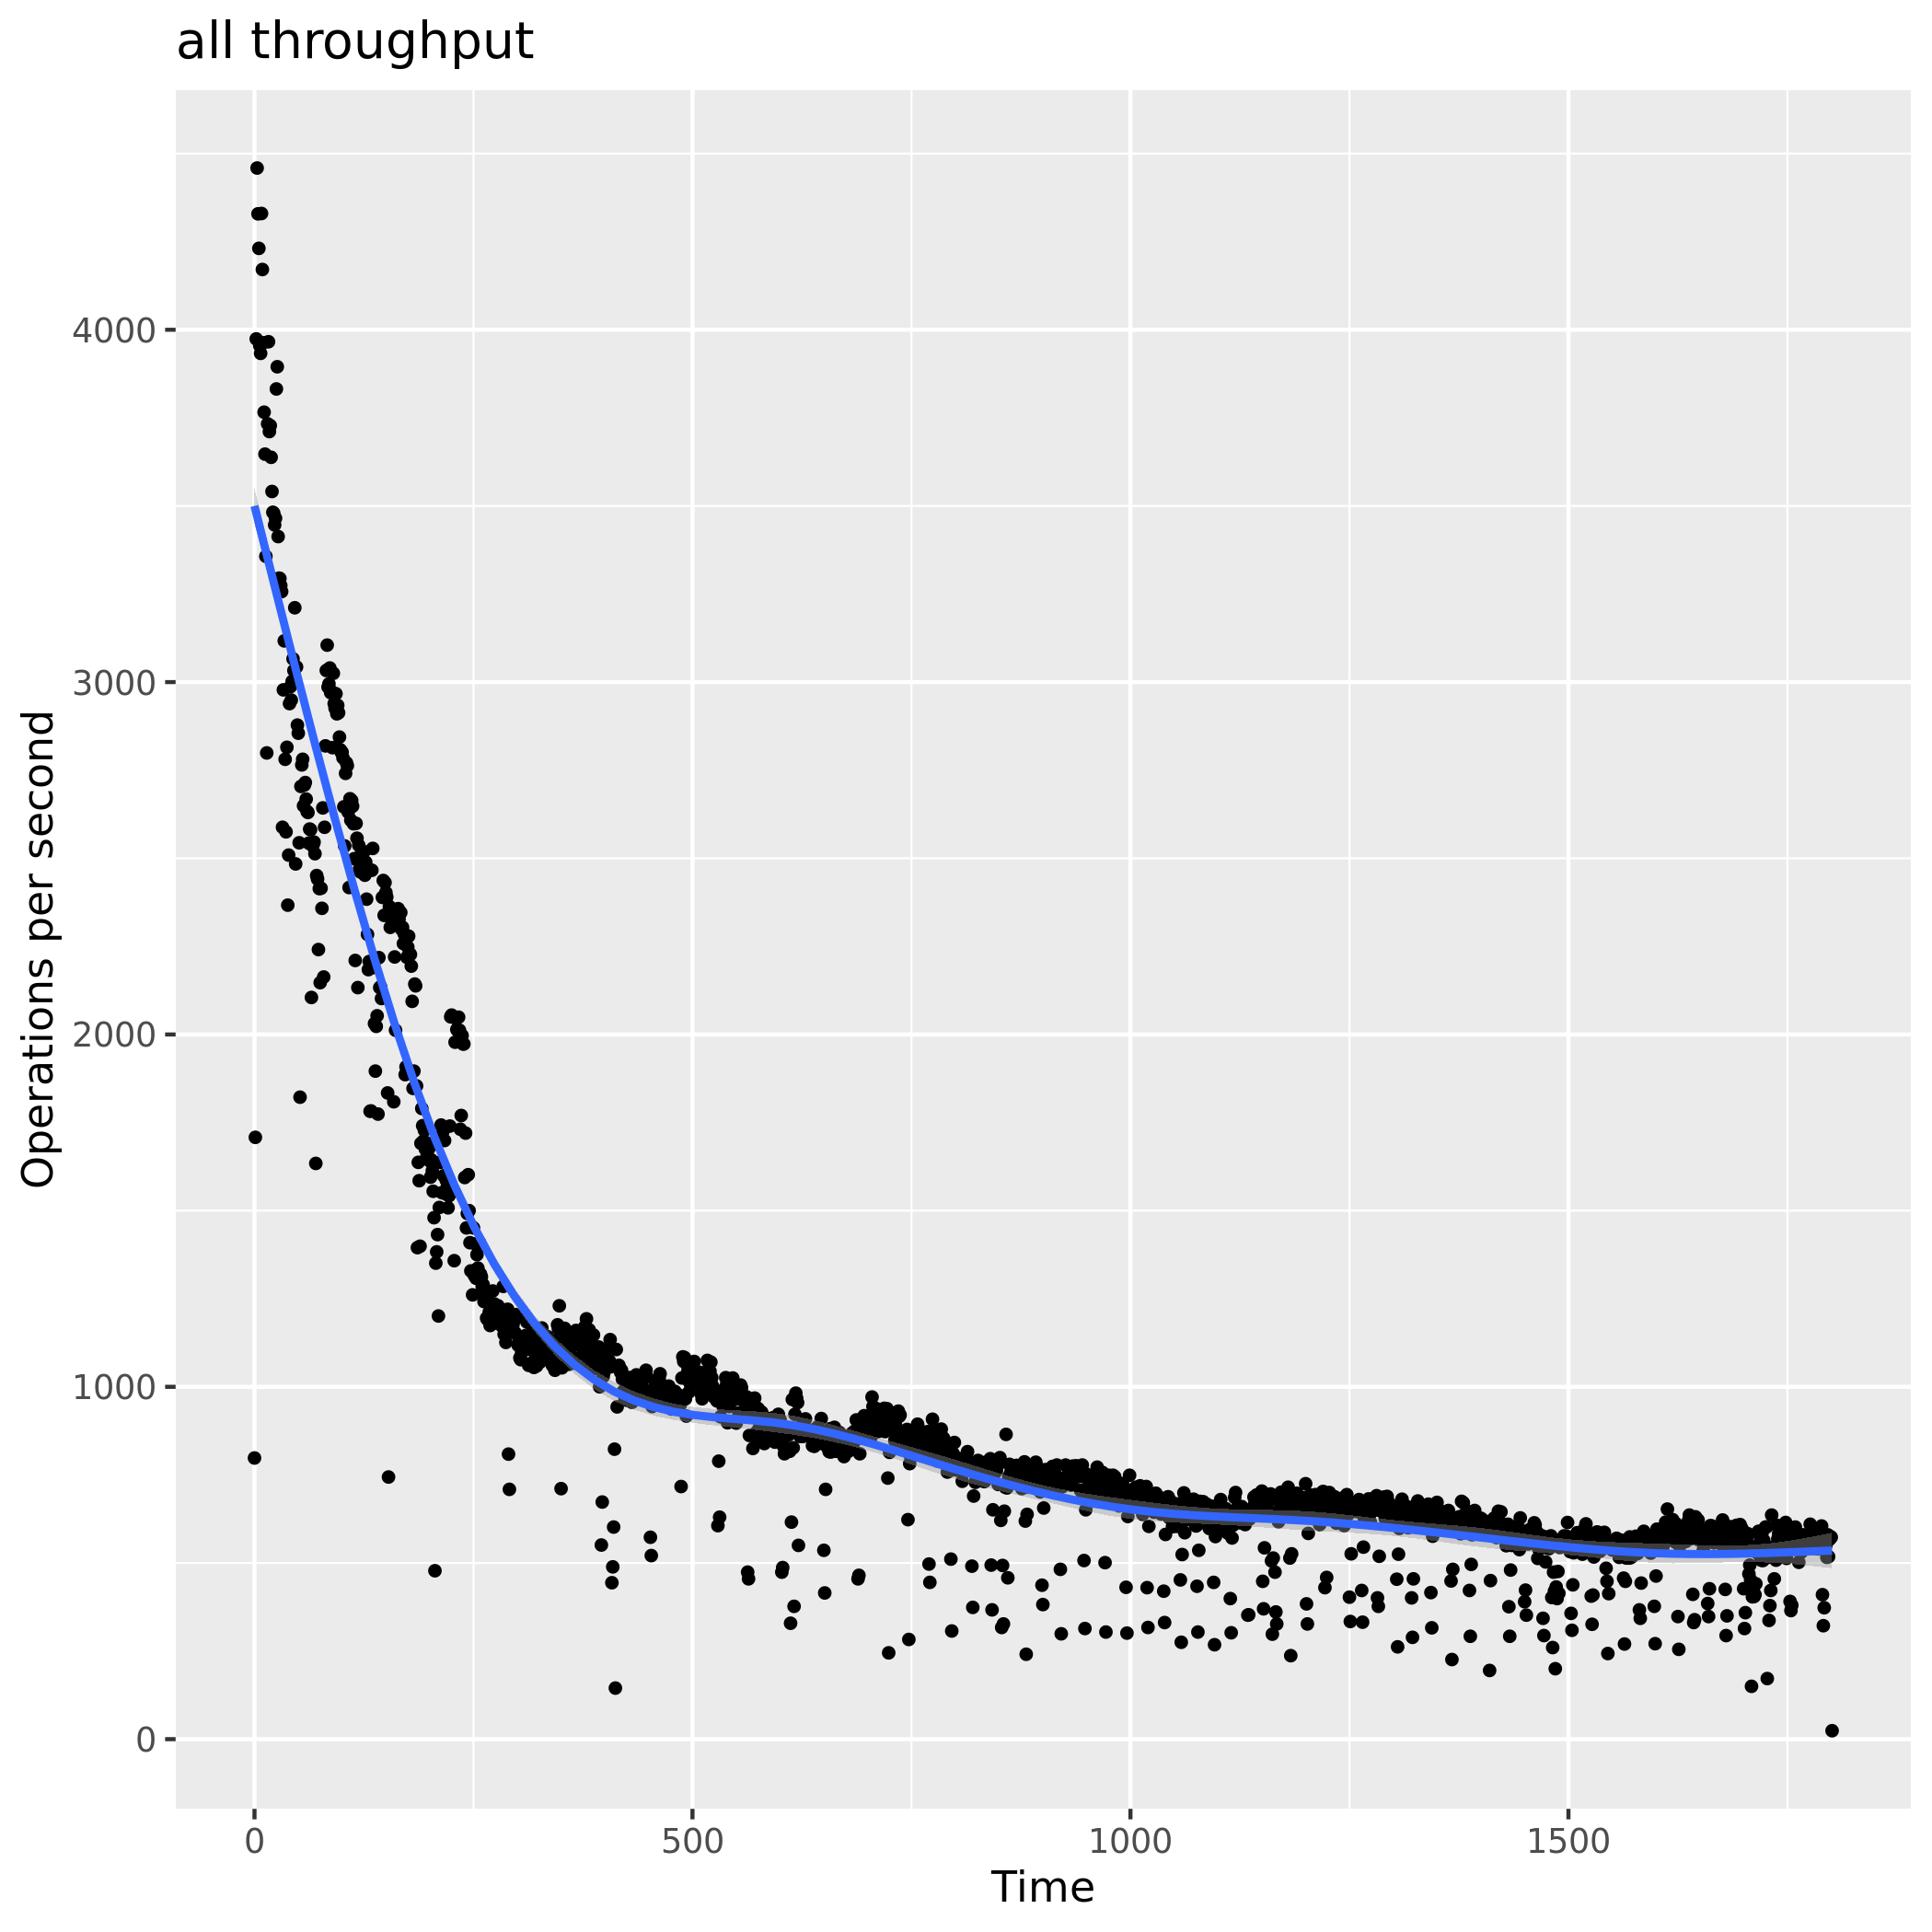
\includegraphics[width=0.8\textwidth]{ConsistentHashing_C0_write_heavy_throughput}
	\caption[Throughput for Consistent Hashing in C0]{Throughput for Consistent Hashing in C0}
\end{subfigure}
\begin{subfigure}{0.5\textwidth}
	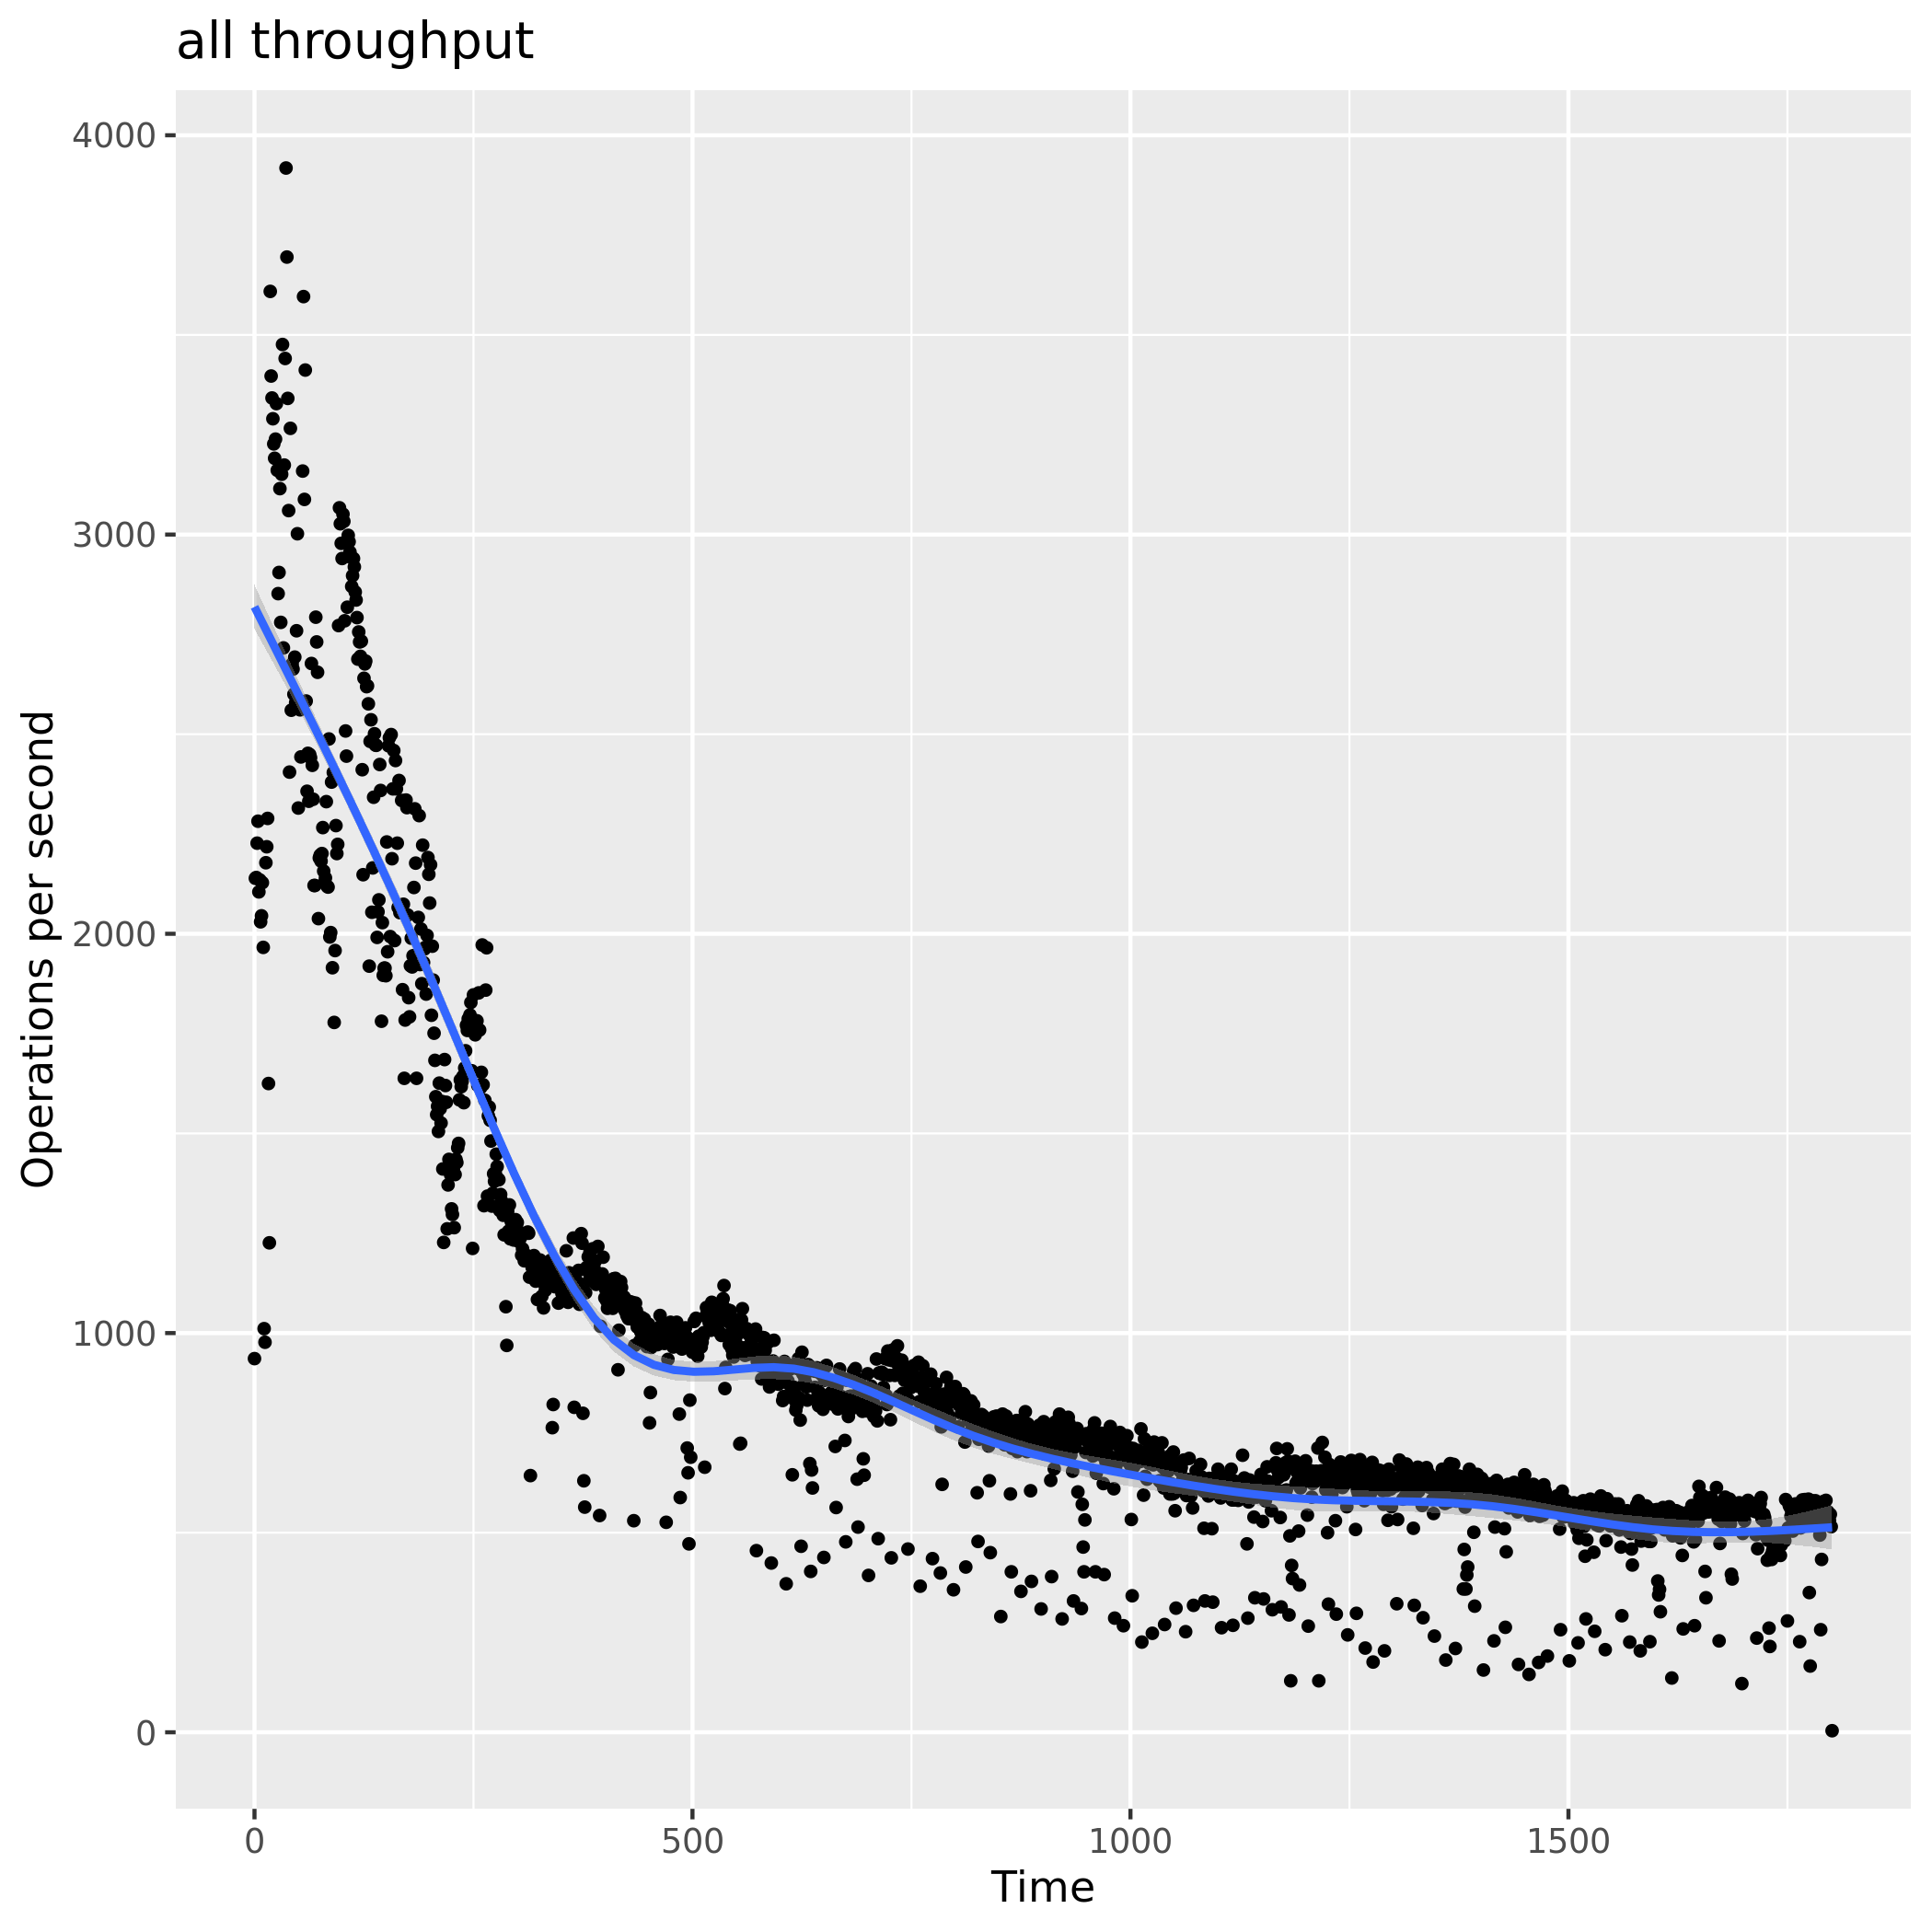
\includegraphics[width=0.8\textwidth]{RandomSlicing_Random_C0_write_heavy_throughput}
	\caption[Throughput for \ac{RS} in C0]{Throughput for \ac{RS} in C0}
\end{subfigure}
\begin{subfigure}{0.5\textwidth}
	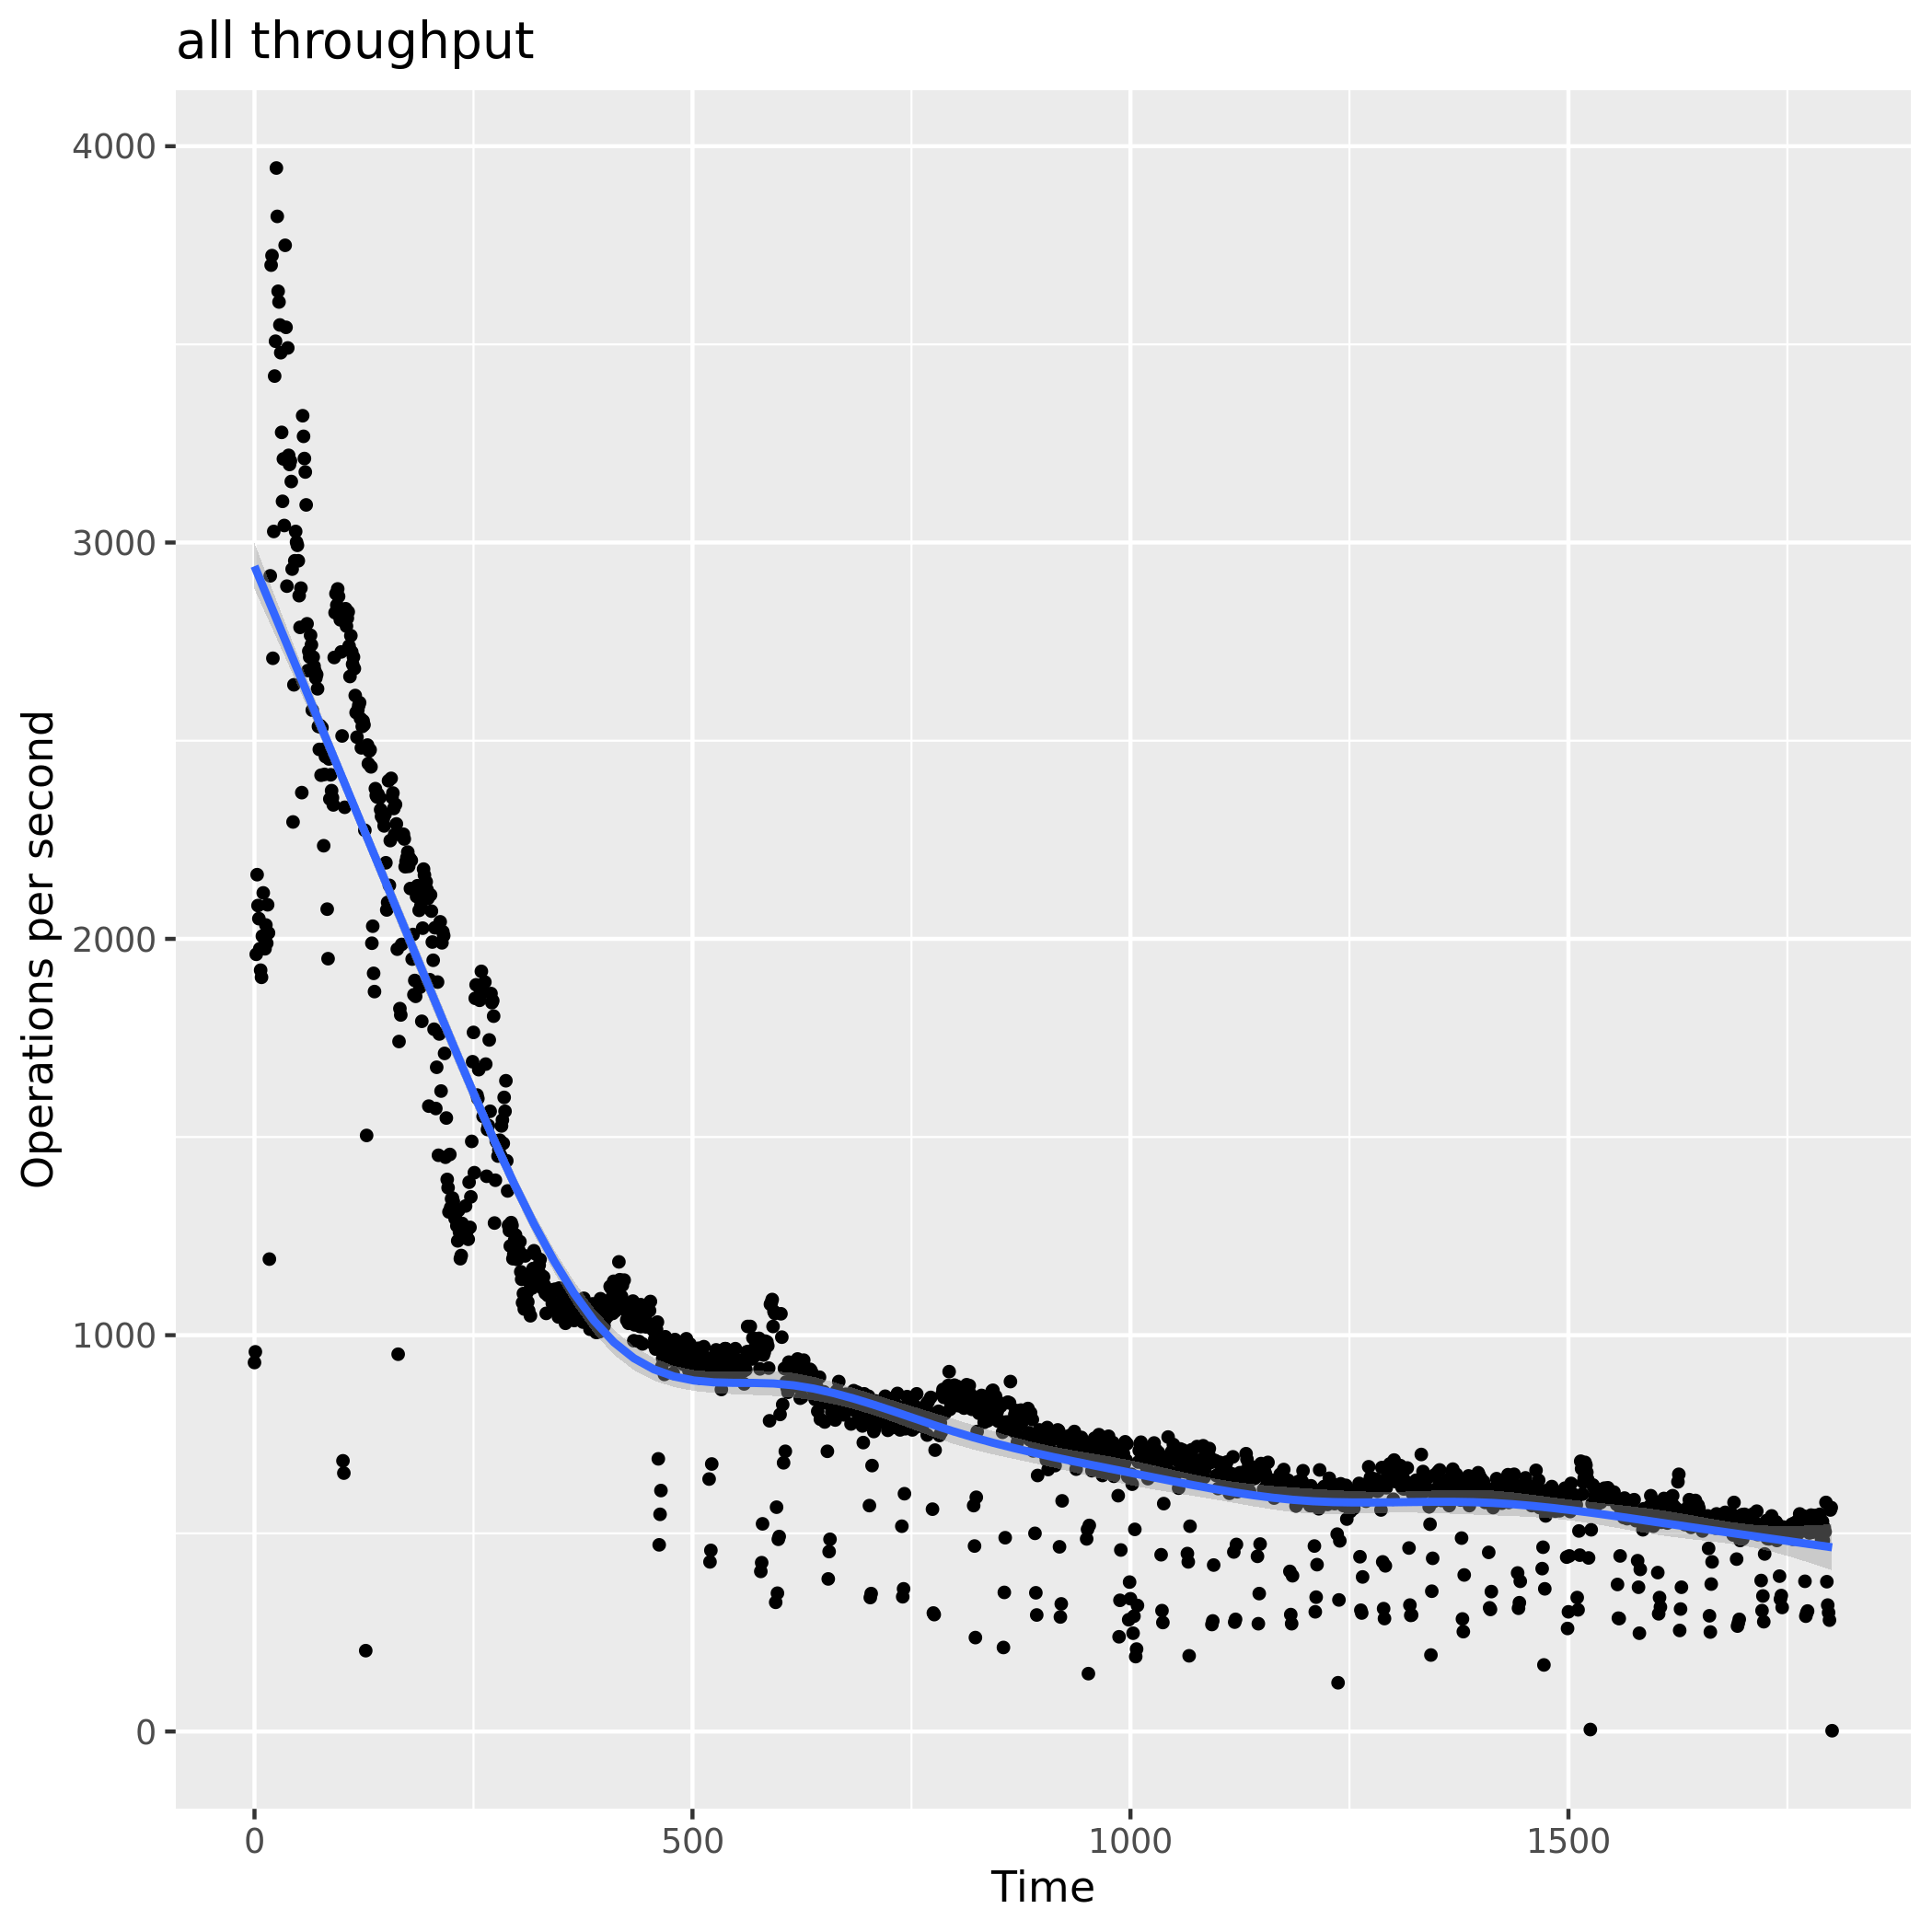
\includegraphics[width=0.8\textwidth]{ConsistentHashing_C1_read_heavy_throughput}
	\caption[Throughput for Consistent Hashing in C1]{Throughput for Consistent Hashing in C1}
\end{subfigure}
\begin{subfigure}{0.5\textwidth}
	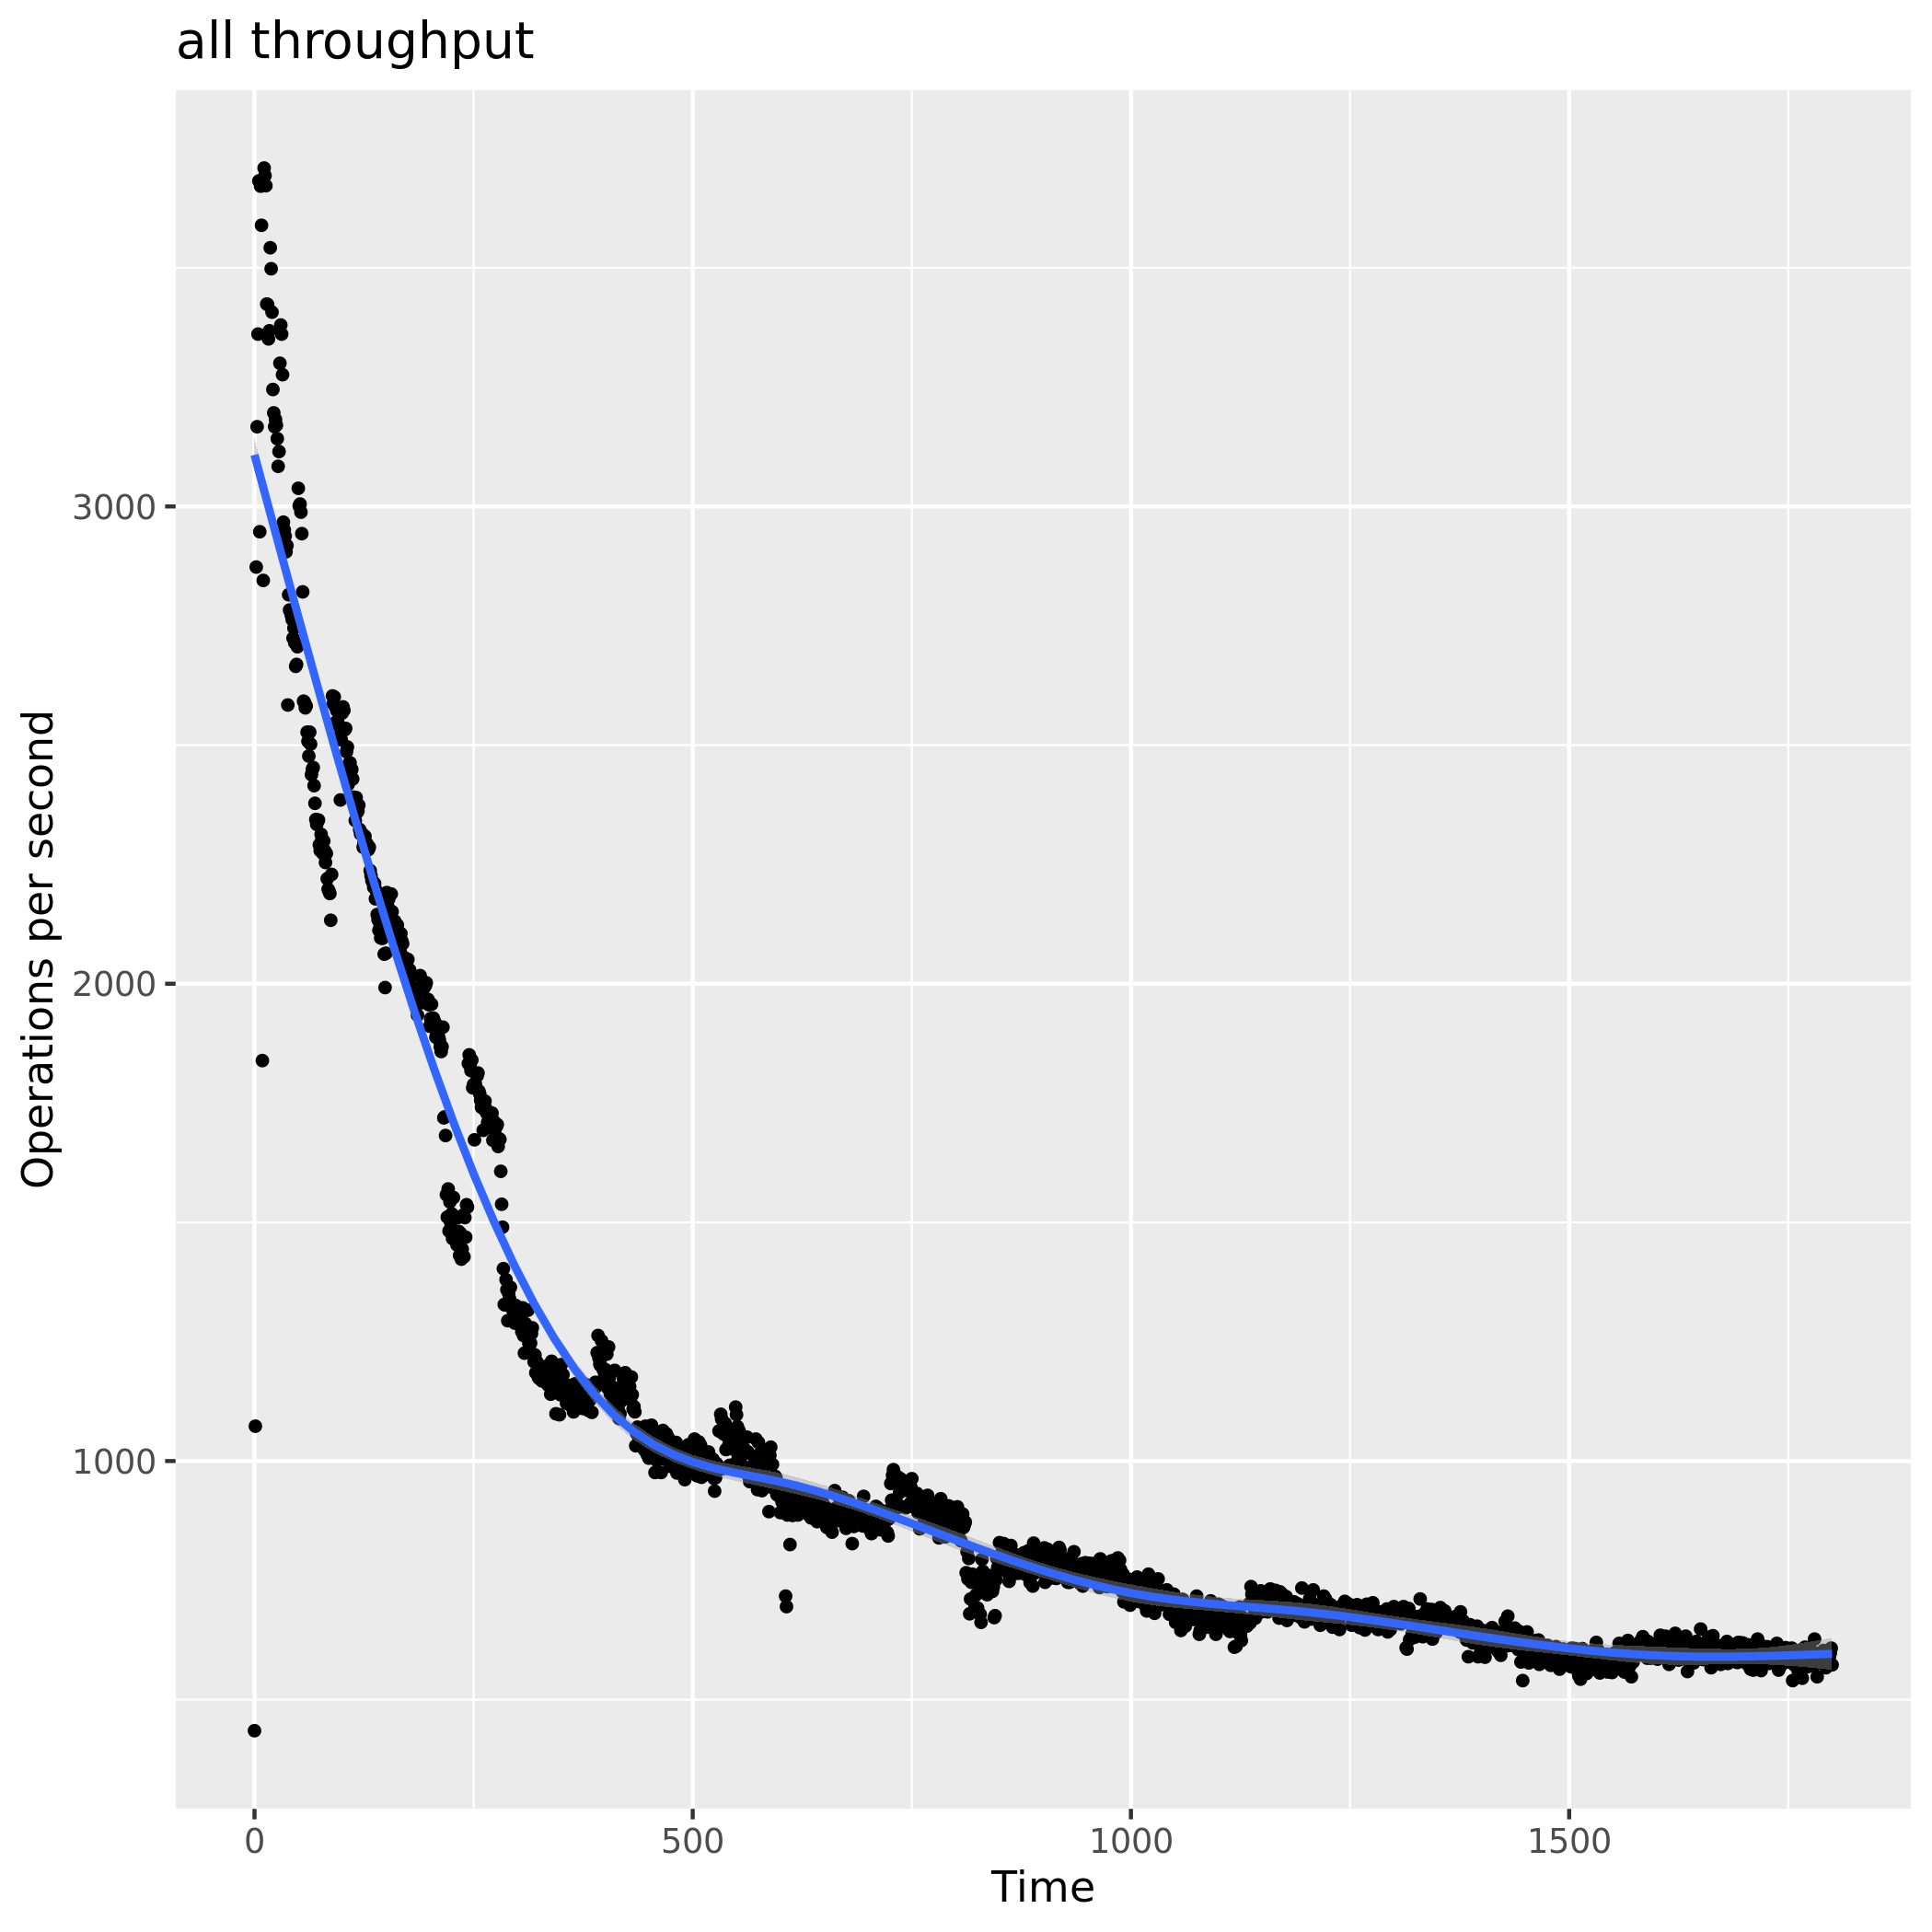
\includegraphics[width=0.8\textwidth]{RandomSlicing_Random_C1_read_heavy_throughput}
	\caption[Throughput for \ac{RS} in C1]{Throughput for \ac{RS} in C1}
\end{subfigure}
\begin{subfigure}{0.5\textwidth}
	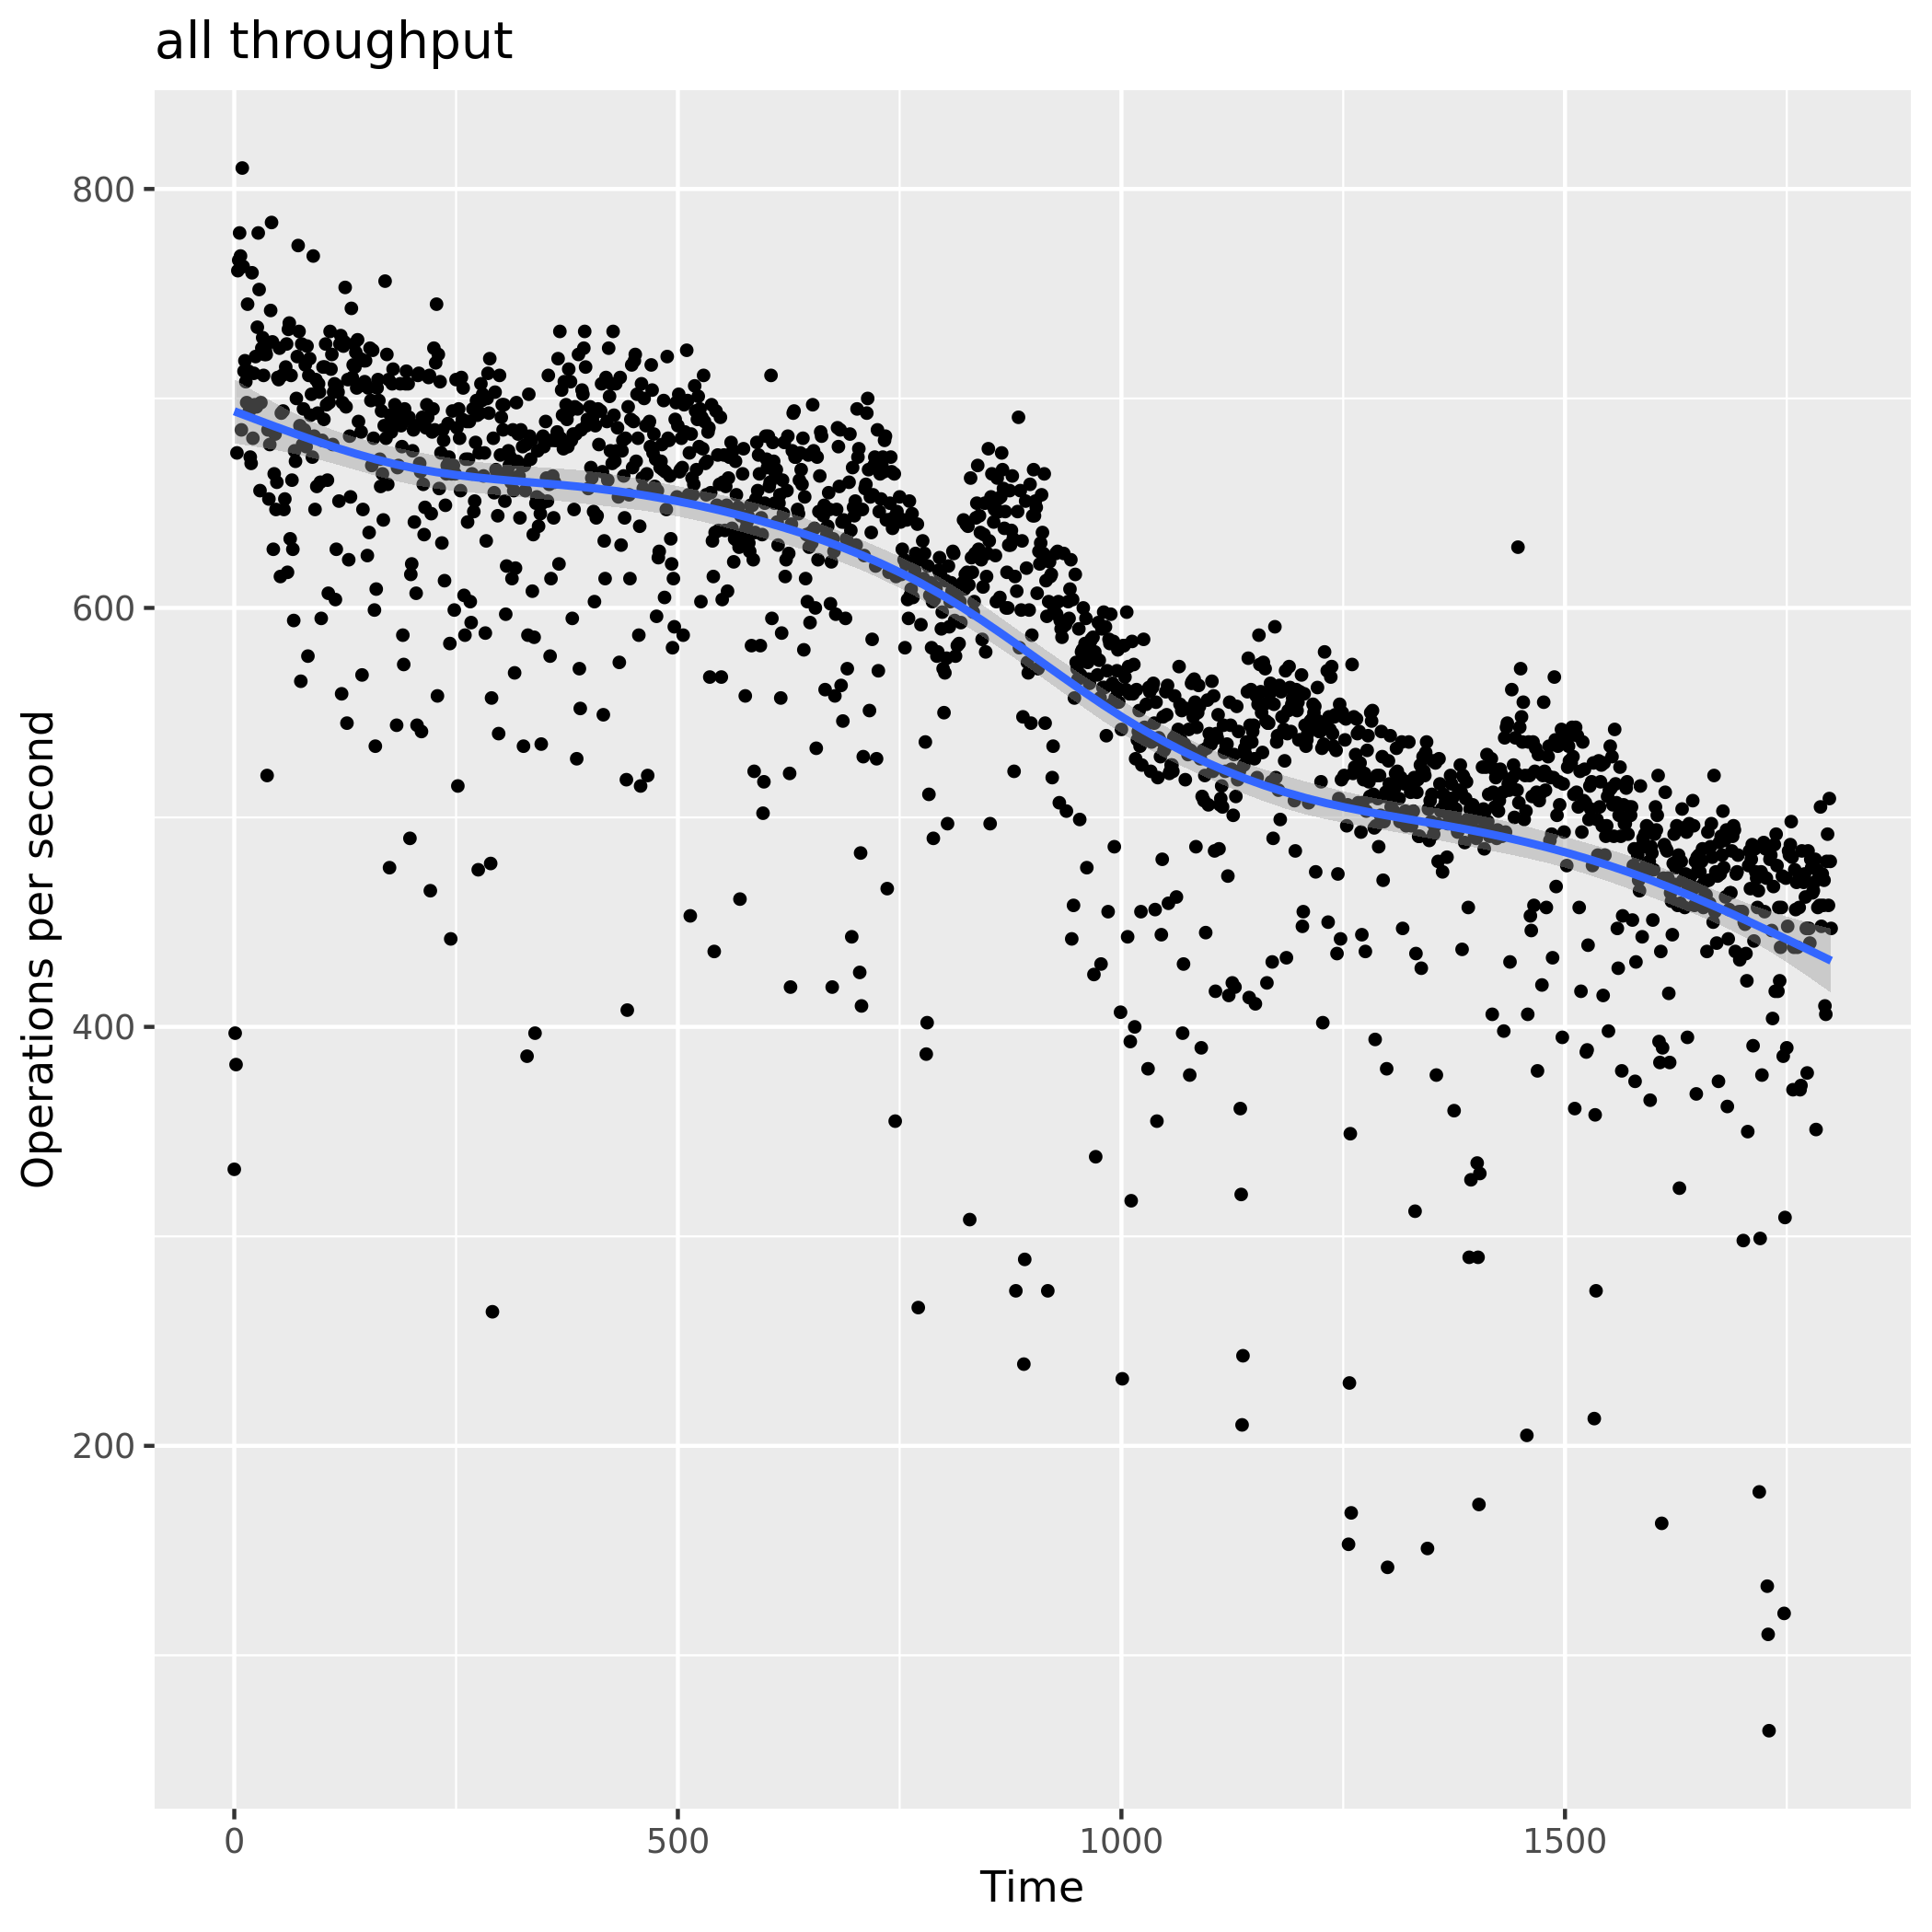
\includegraphics[width=0.8\textwidth]{ConsistentHashing_C2_write_heavy_throughput}
	\caption[Throughput for Consistent Hashing in C2]{Throughput for Consistent Hashing in C2}
\end{subfigure}
\begin{subfigure}{0.5\textwidth}
	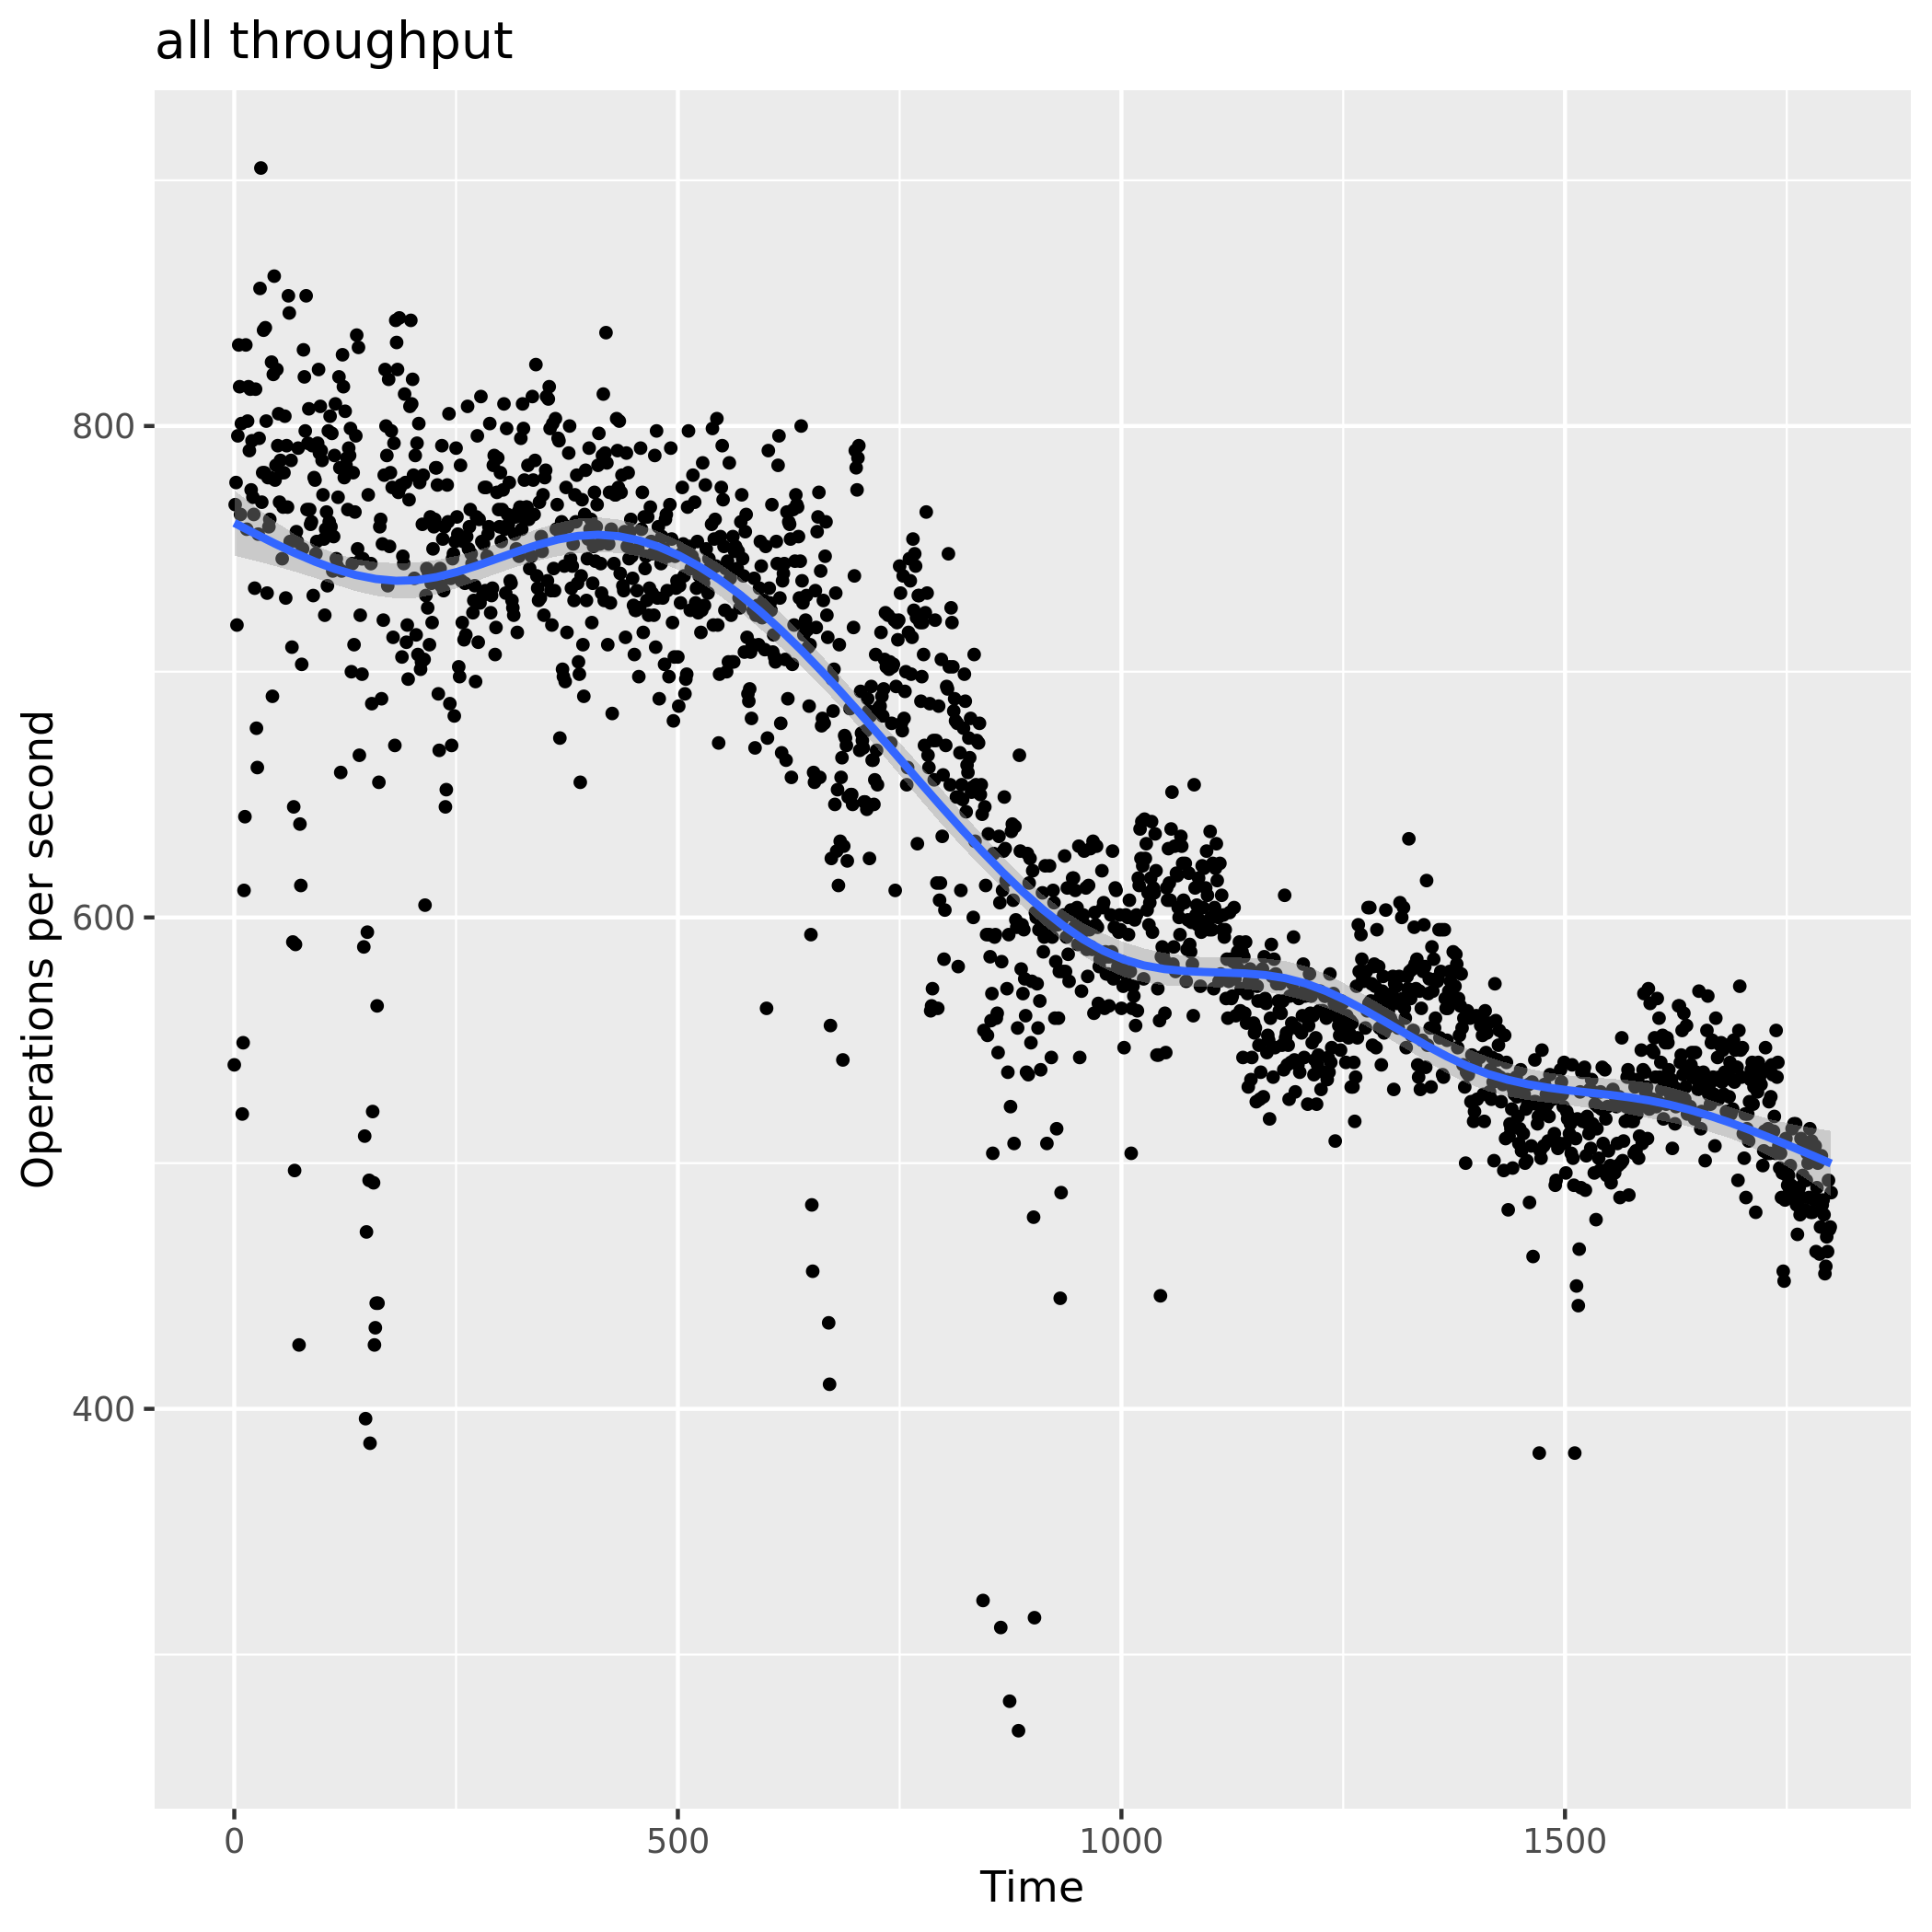
\includegraphics[width=0.8\textwidth]{RandomSlicing_Random_C2_write_heavy_throughput}
	\caption[Throughput for \ac{RS} in C2]{Throughput for \ac{RS} in C2}
\end{subfigure}
\caption[Throughput Comparison]{Throughput Comparison. On the left are the throughput plots of Consistent Hashing, on the right the ones of \ac{RS}.}
\label{fig:throughput_comparison}
\end{figure}
Therefore the hypothesis can be seen as plausible.

\subsubsection{Hypothesis 5}
Hypothesis 5 claims that a system with \ac{RS} will recover faster after a cluster change than with Consistent Hashing.
Again we are using Random Replication as the replication placement strategy to enable a fair comparison.
As the behavior of the throughput during handoff operations is quite unexpected it is hard to tell from its plot when a system has actually recovered.
However, there are clear edges in the latency plots that can be used to approximate the duration of system disruption.
The latency plots of the dynamic runs can be seen in \cref{fig:handoff_comparison}.
\begin{figure}
\begin{subfigure}{0.5\textwidth}
	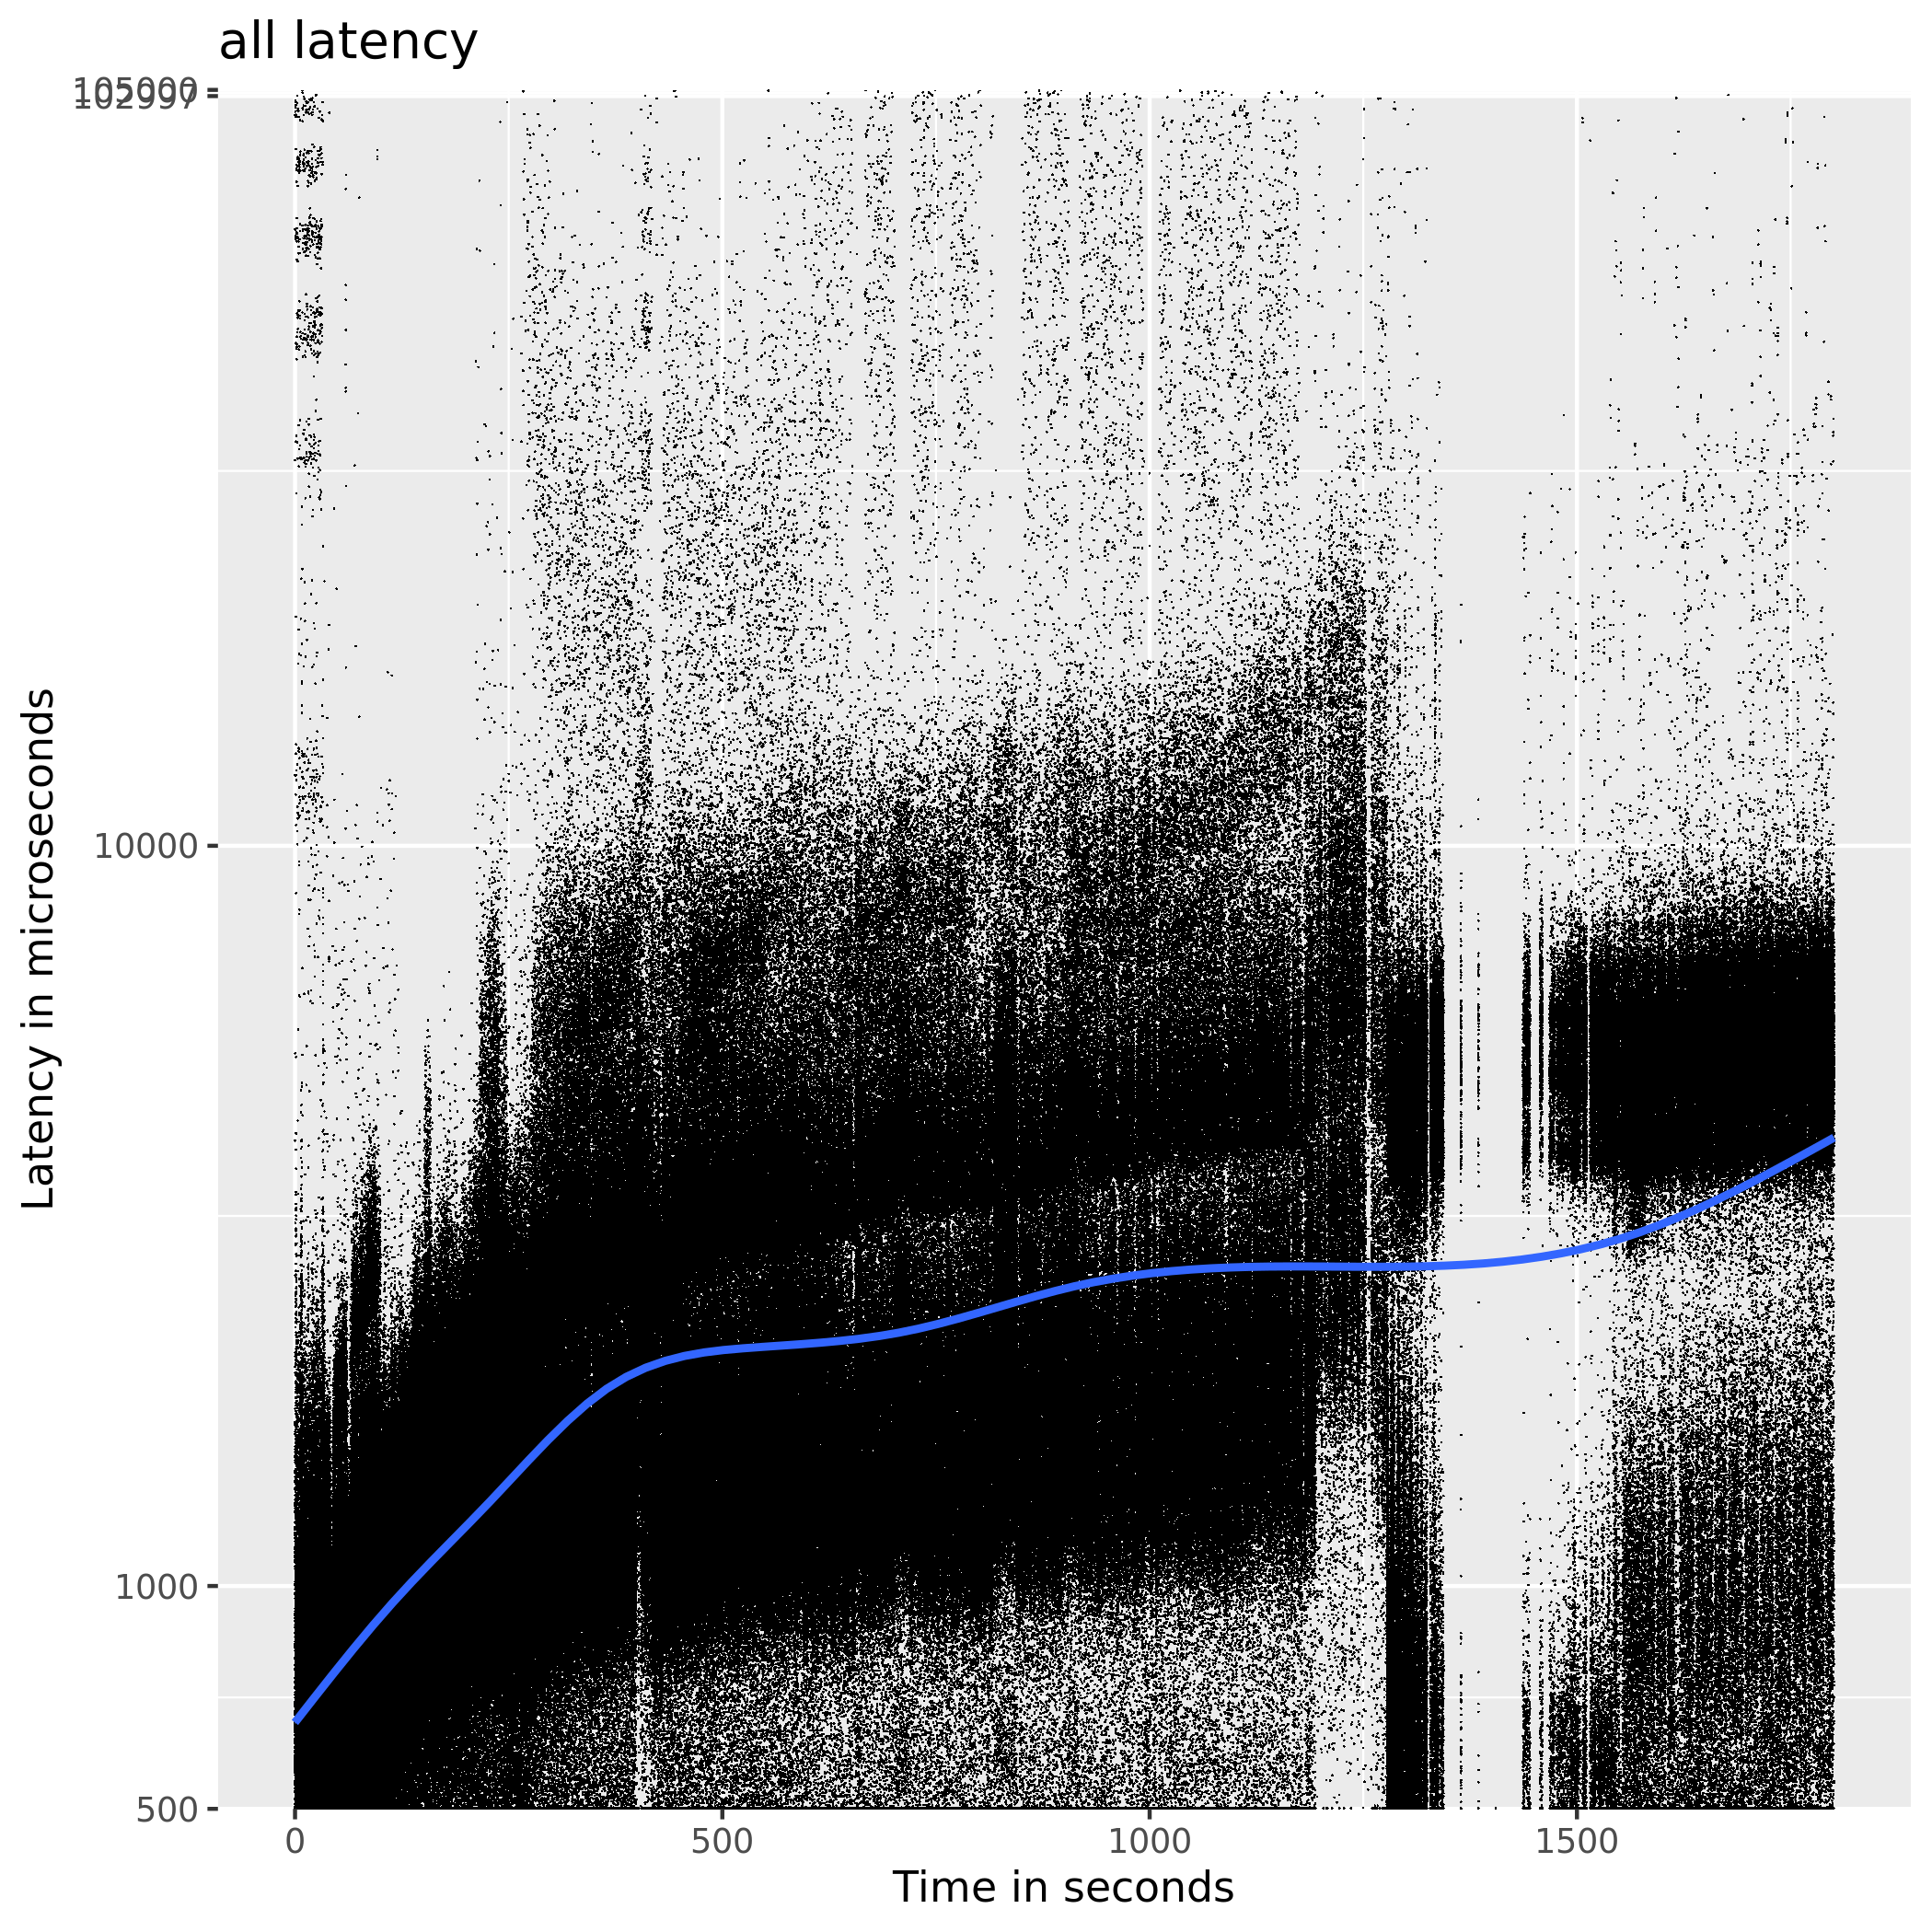
\includegraphics[width=0.8\textwidth]{ConsistentHashing_dynamic_read_heavy_latency}
	\caption[Latency for Consistent Hashing with Read-Heavy Workload]{Latency for Consistent Hashing with Read-Heavy Workload}
\end{subfigure}
\begin{subfigure}{0.5\textwidth}
	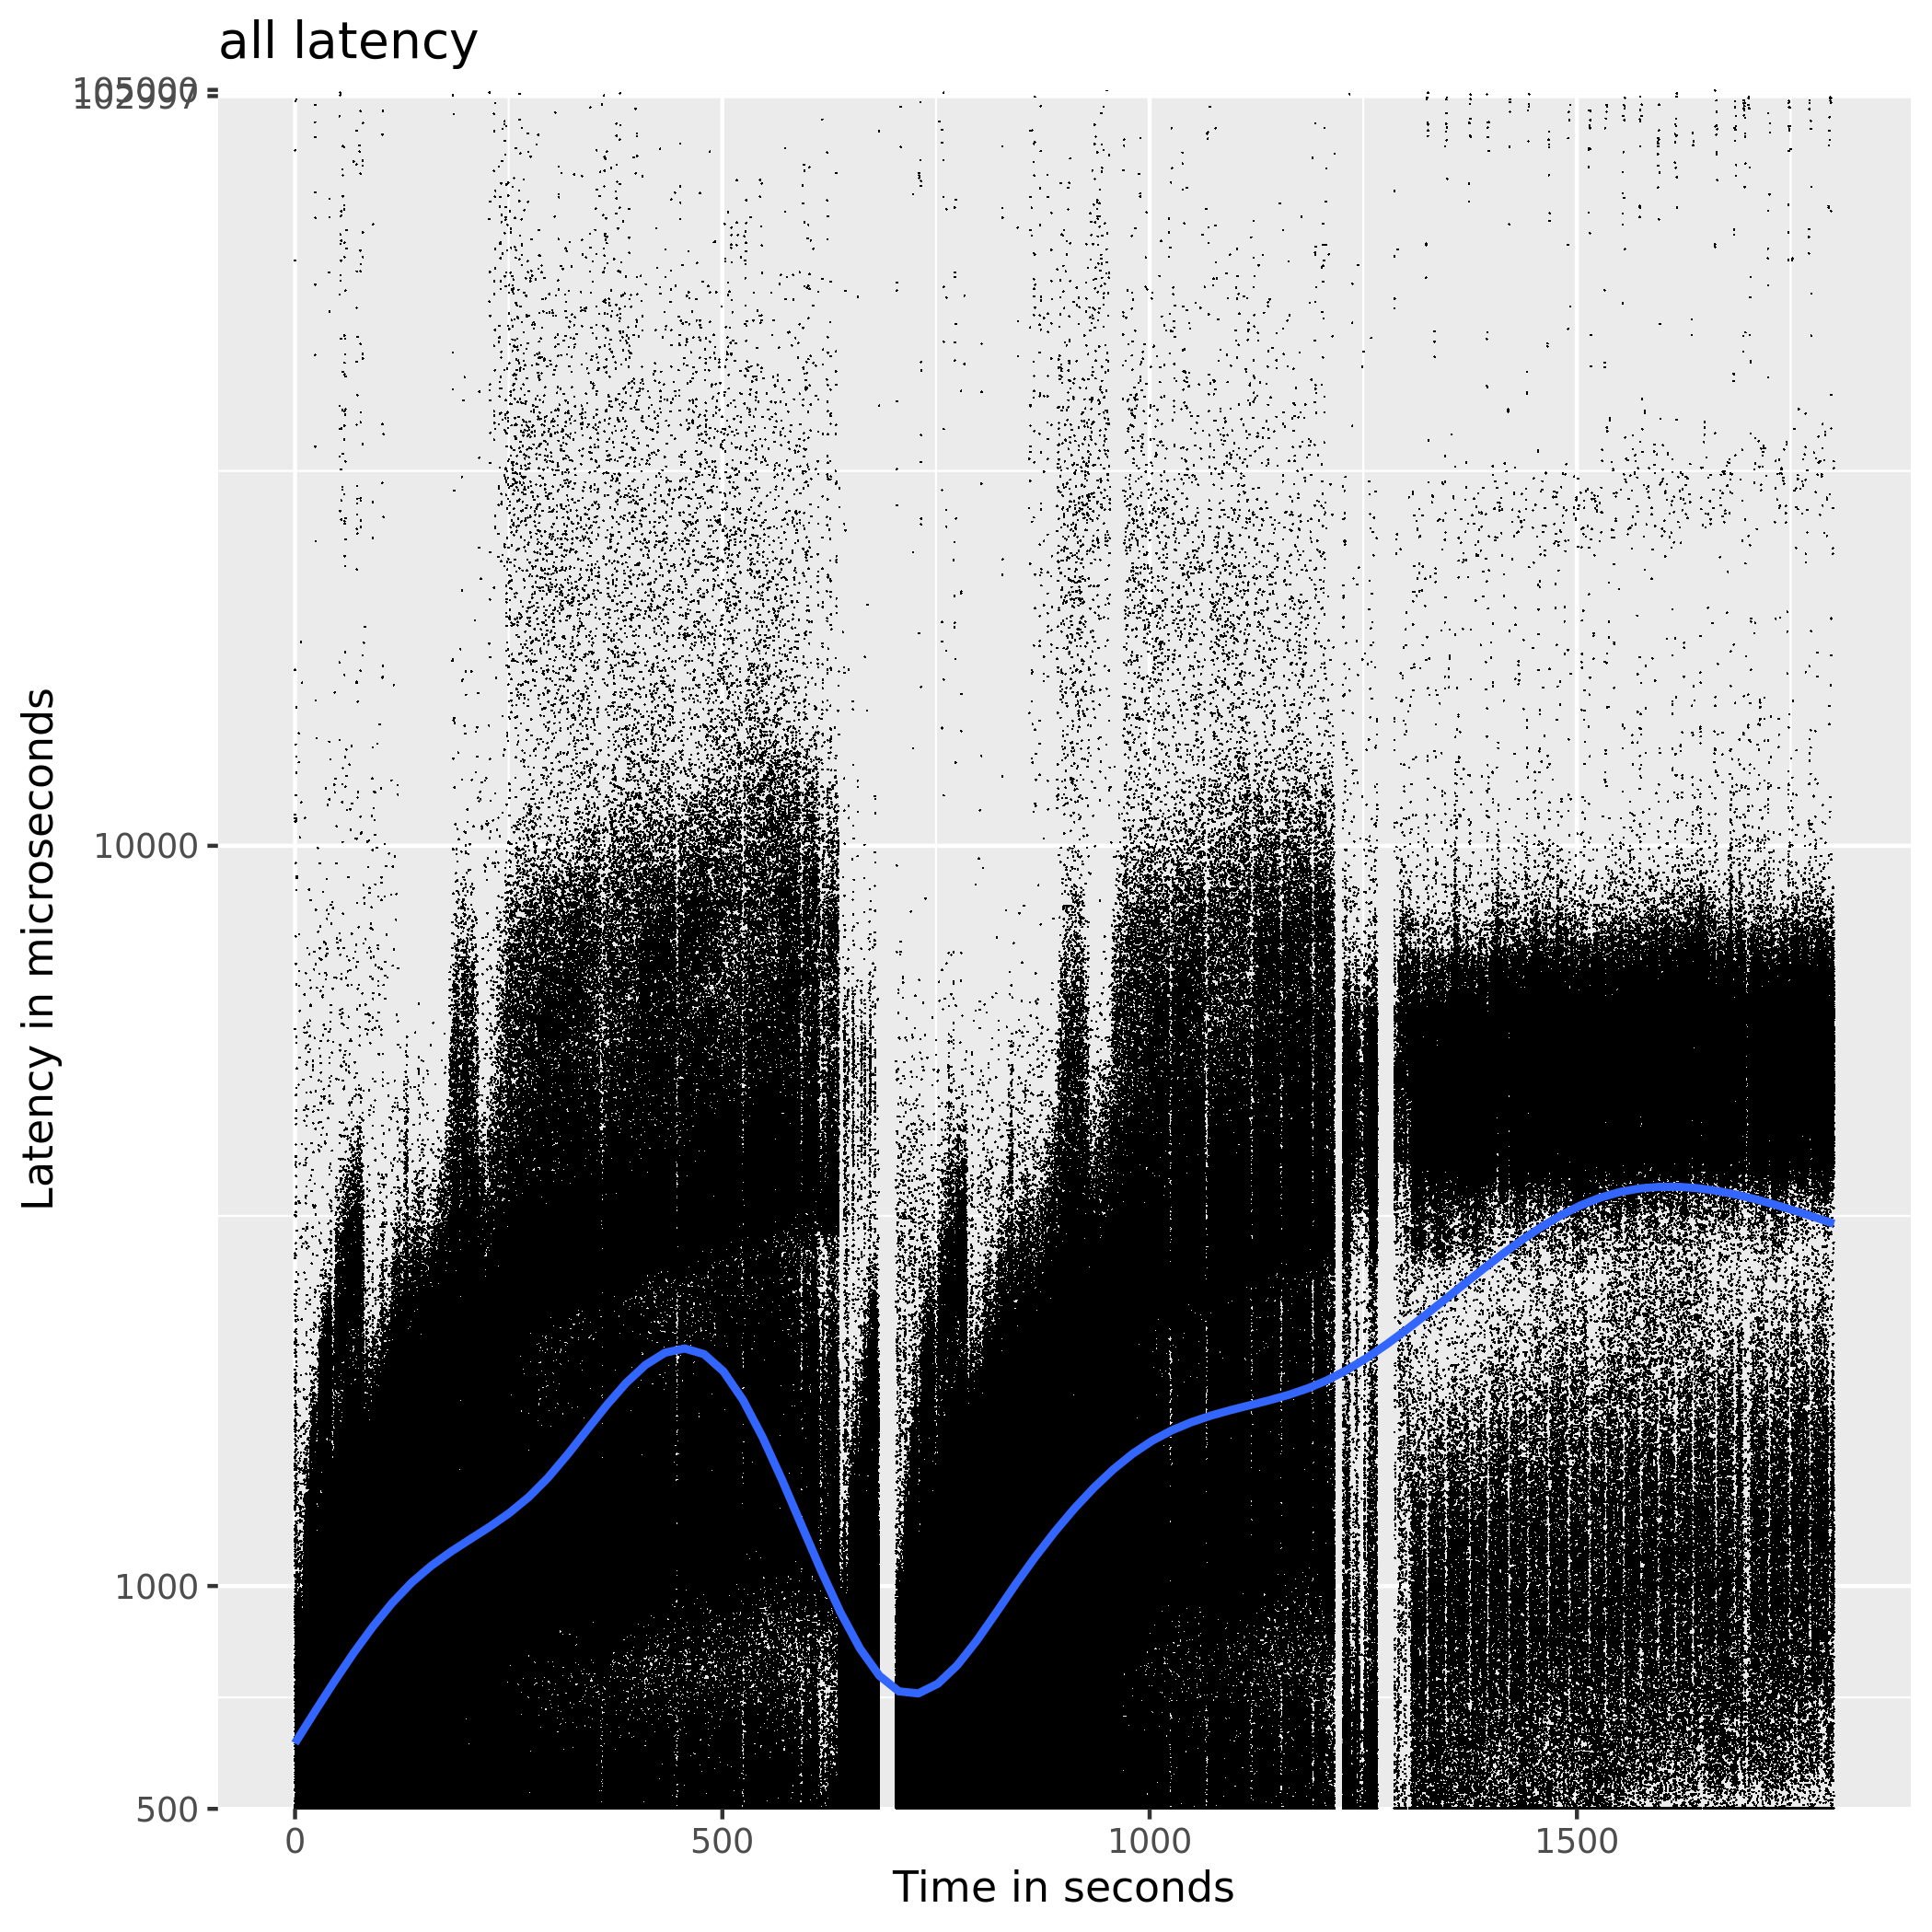
\includegraphics[width=0.8\textwidth]{ConsistentHashing_dynamic_write_heavy_latency}
	\caption[Latency for Consistent Hashing with Write-Heavy Workload]{Latency for Consistent Hashing with Write-Heavy Workload}
\end{subfigure}
\begin{subfigure}{0.5\textwidth}
	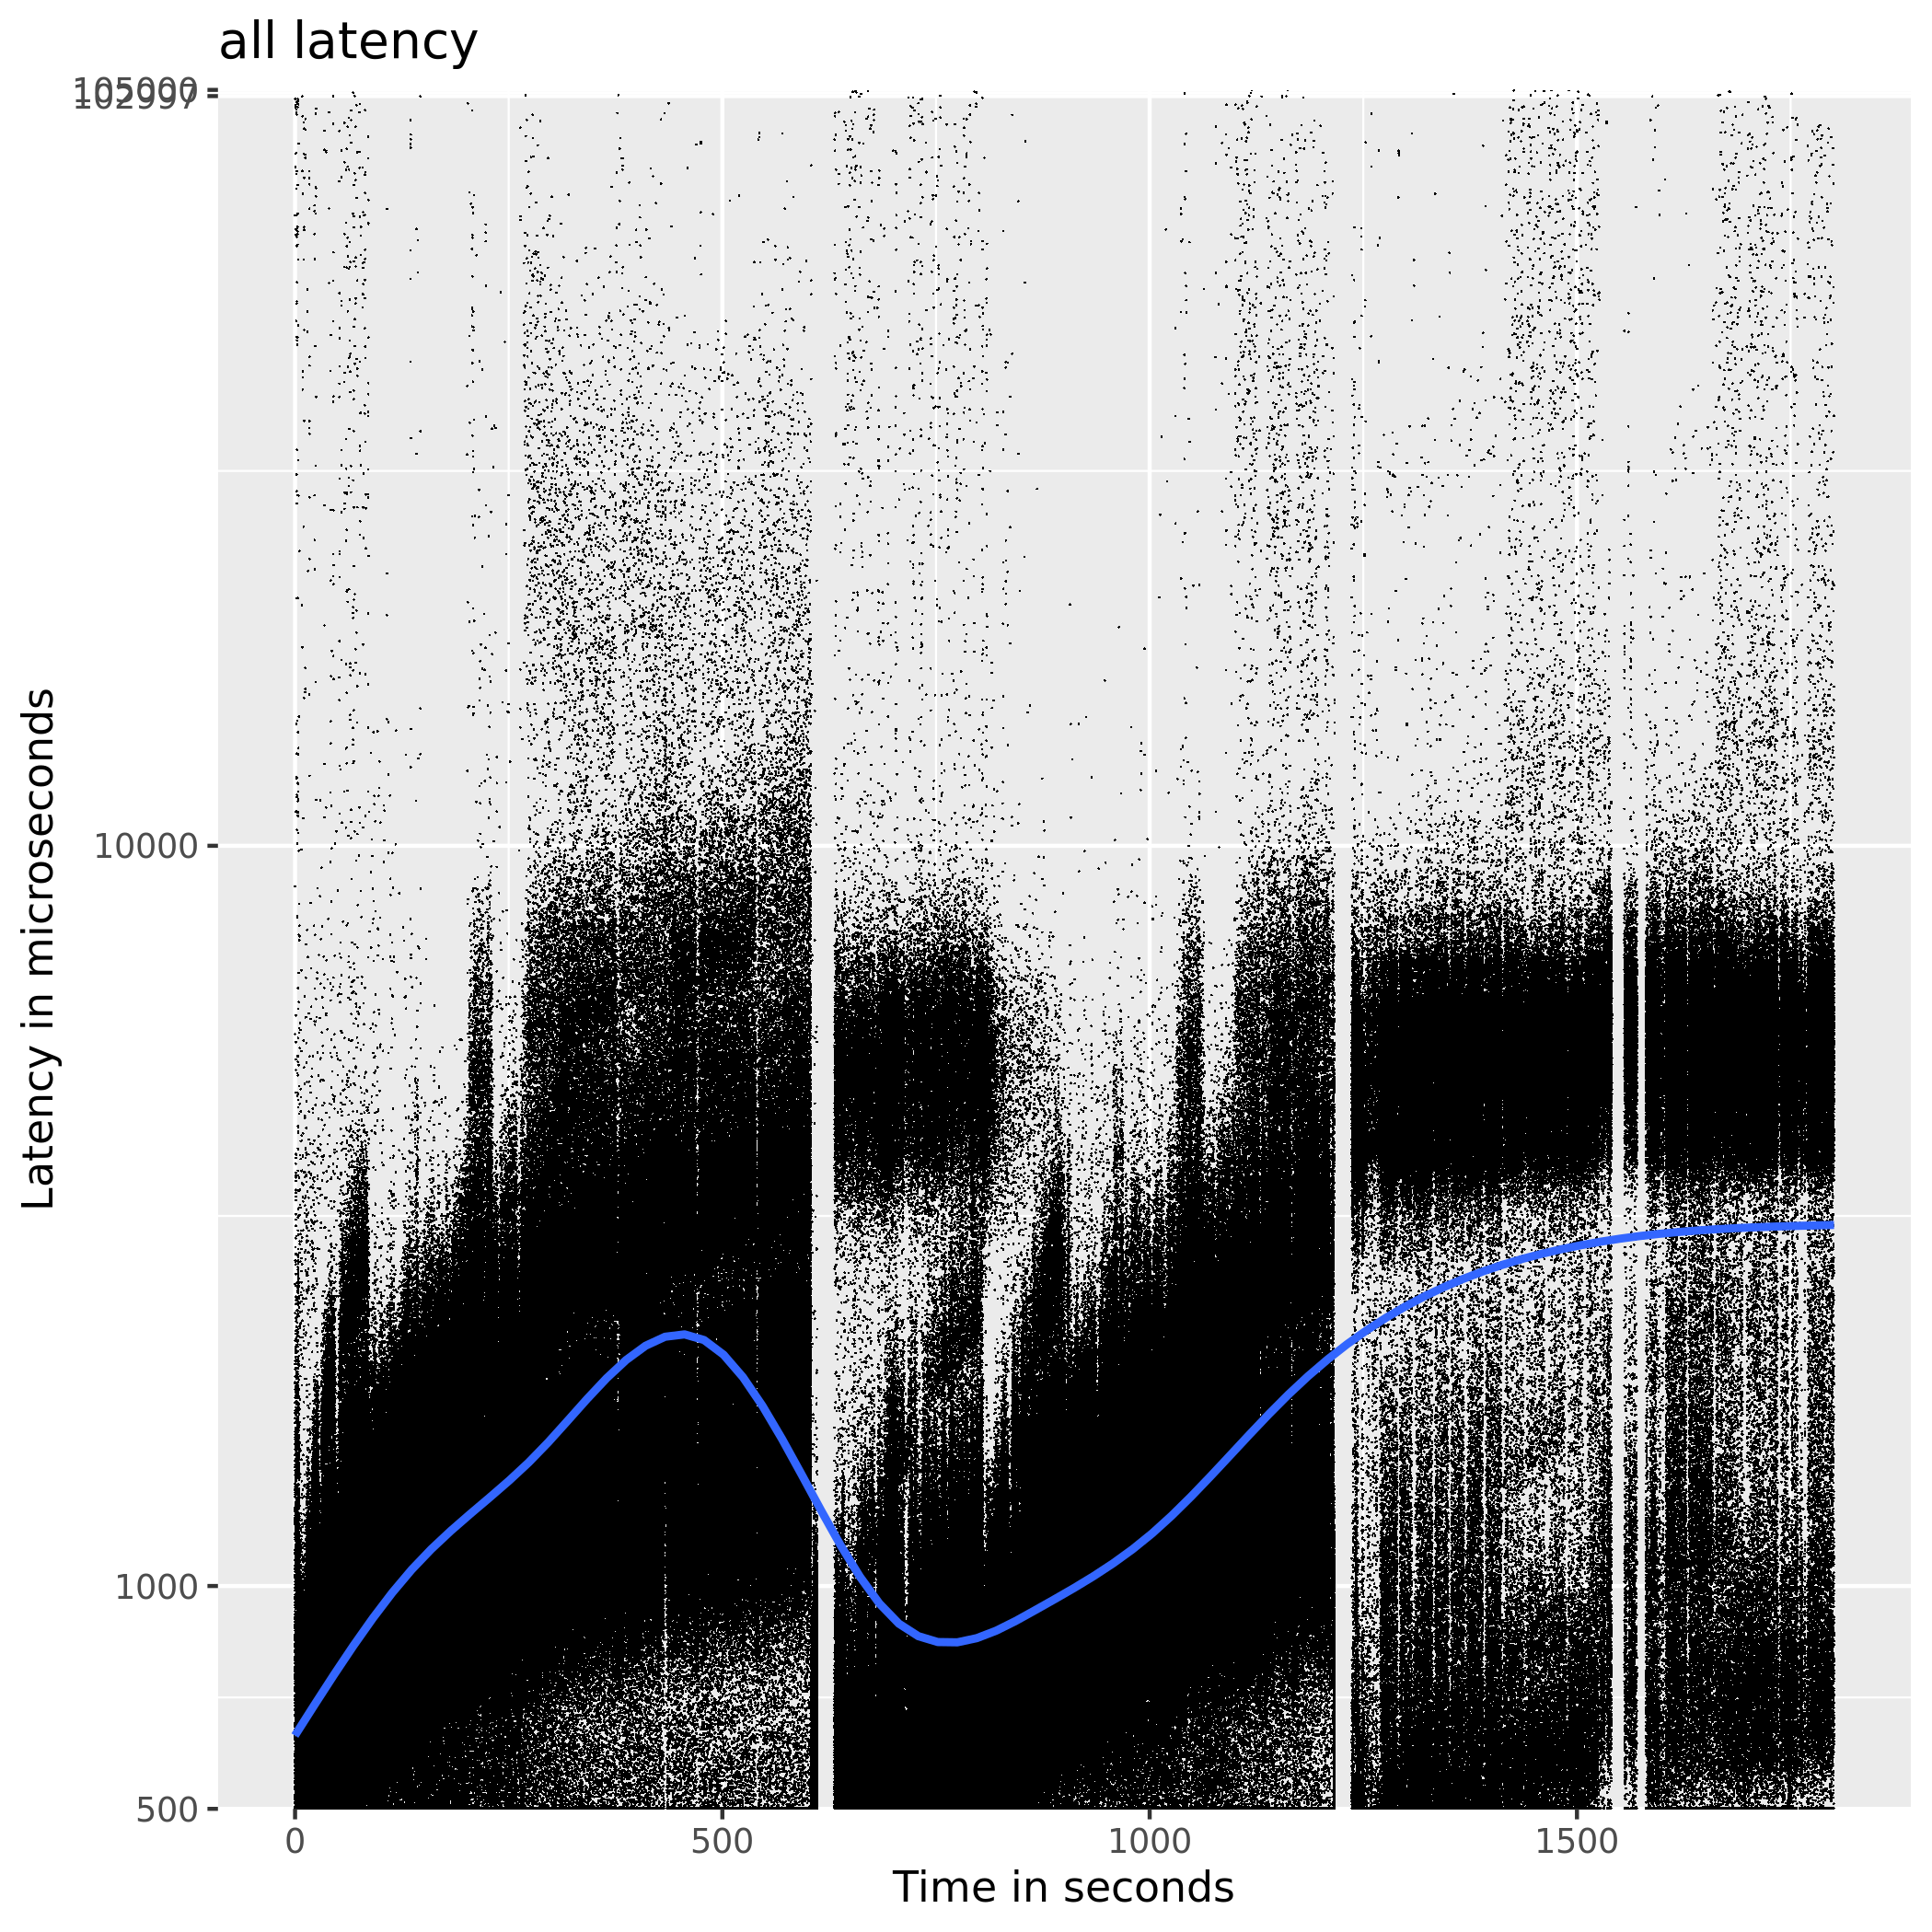
\includegraphics[width=0.8\textwidth]{RandomSlicing_Random_dynamic_read_heavy_latency}
	\caption[Latency for \ac{RS} with Read-Heavy Workload]{Latency for \ac{RS} with Read-Heavy Workload}
\end{subfigure}
\begin{subfigure}{0.5\textwidth}
	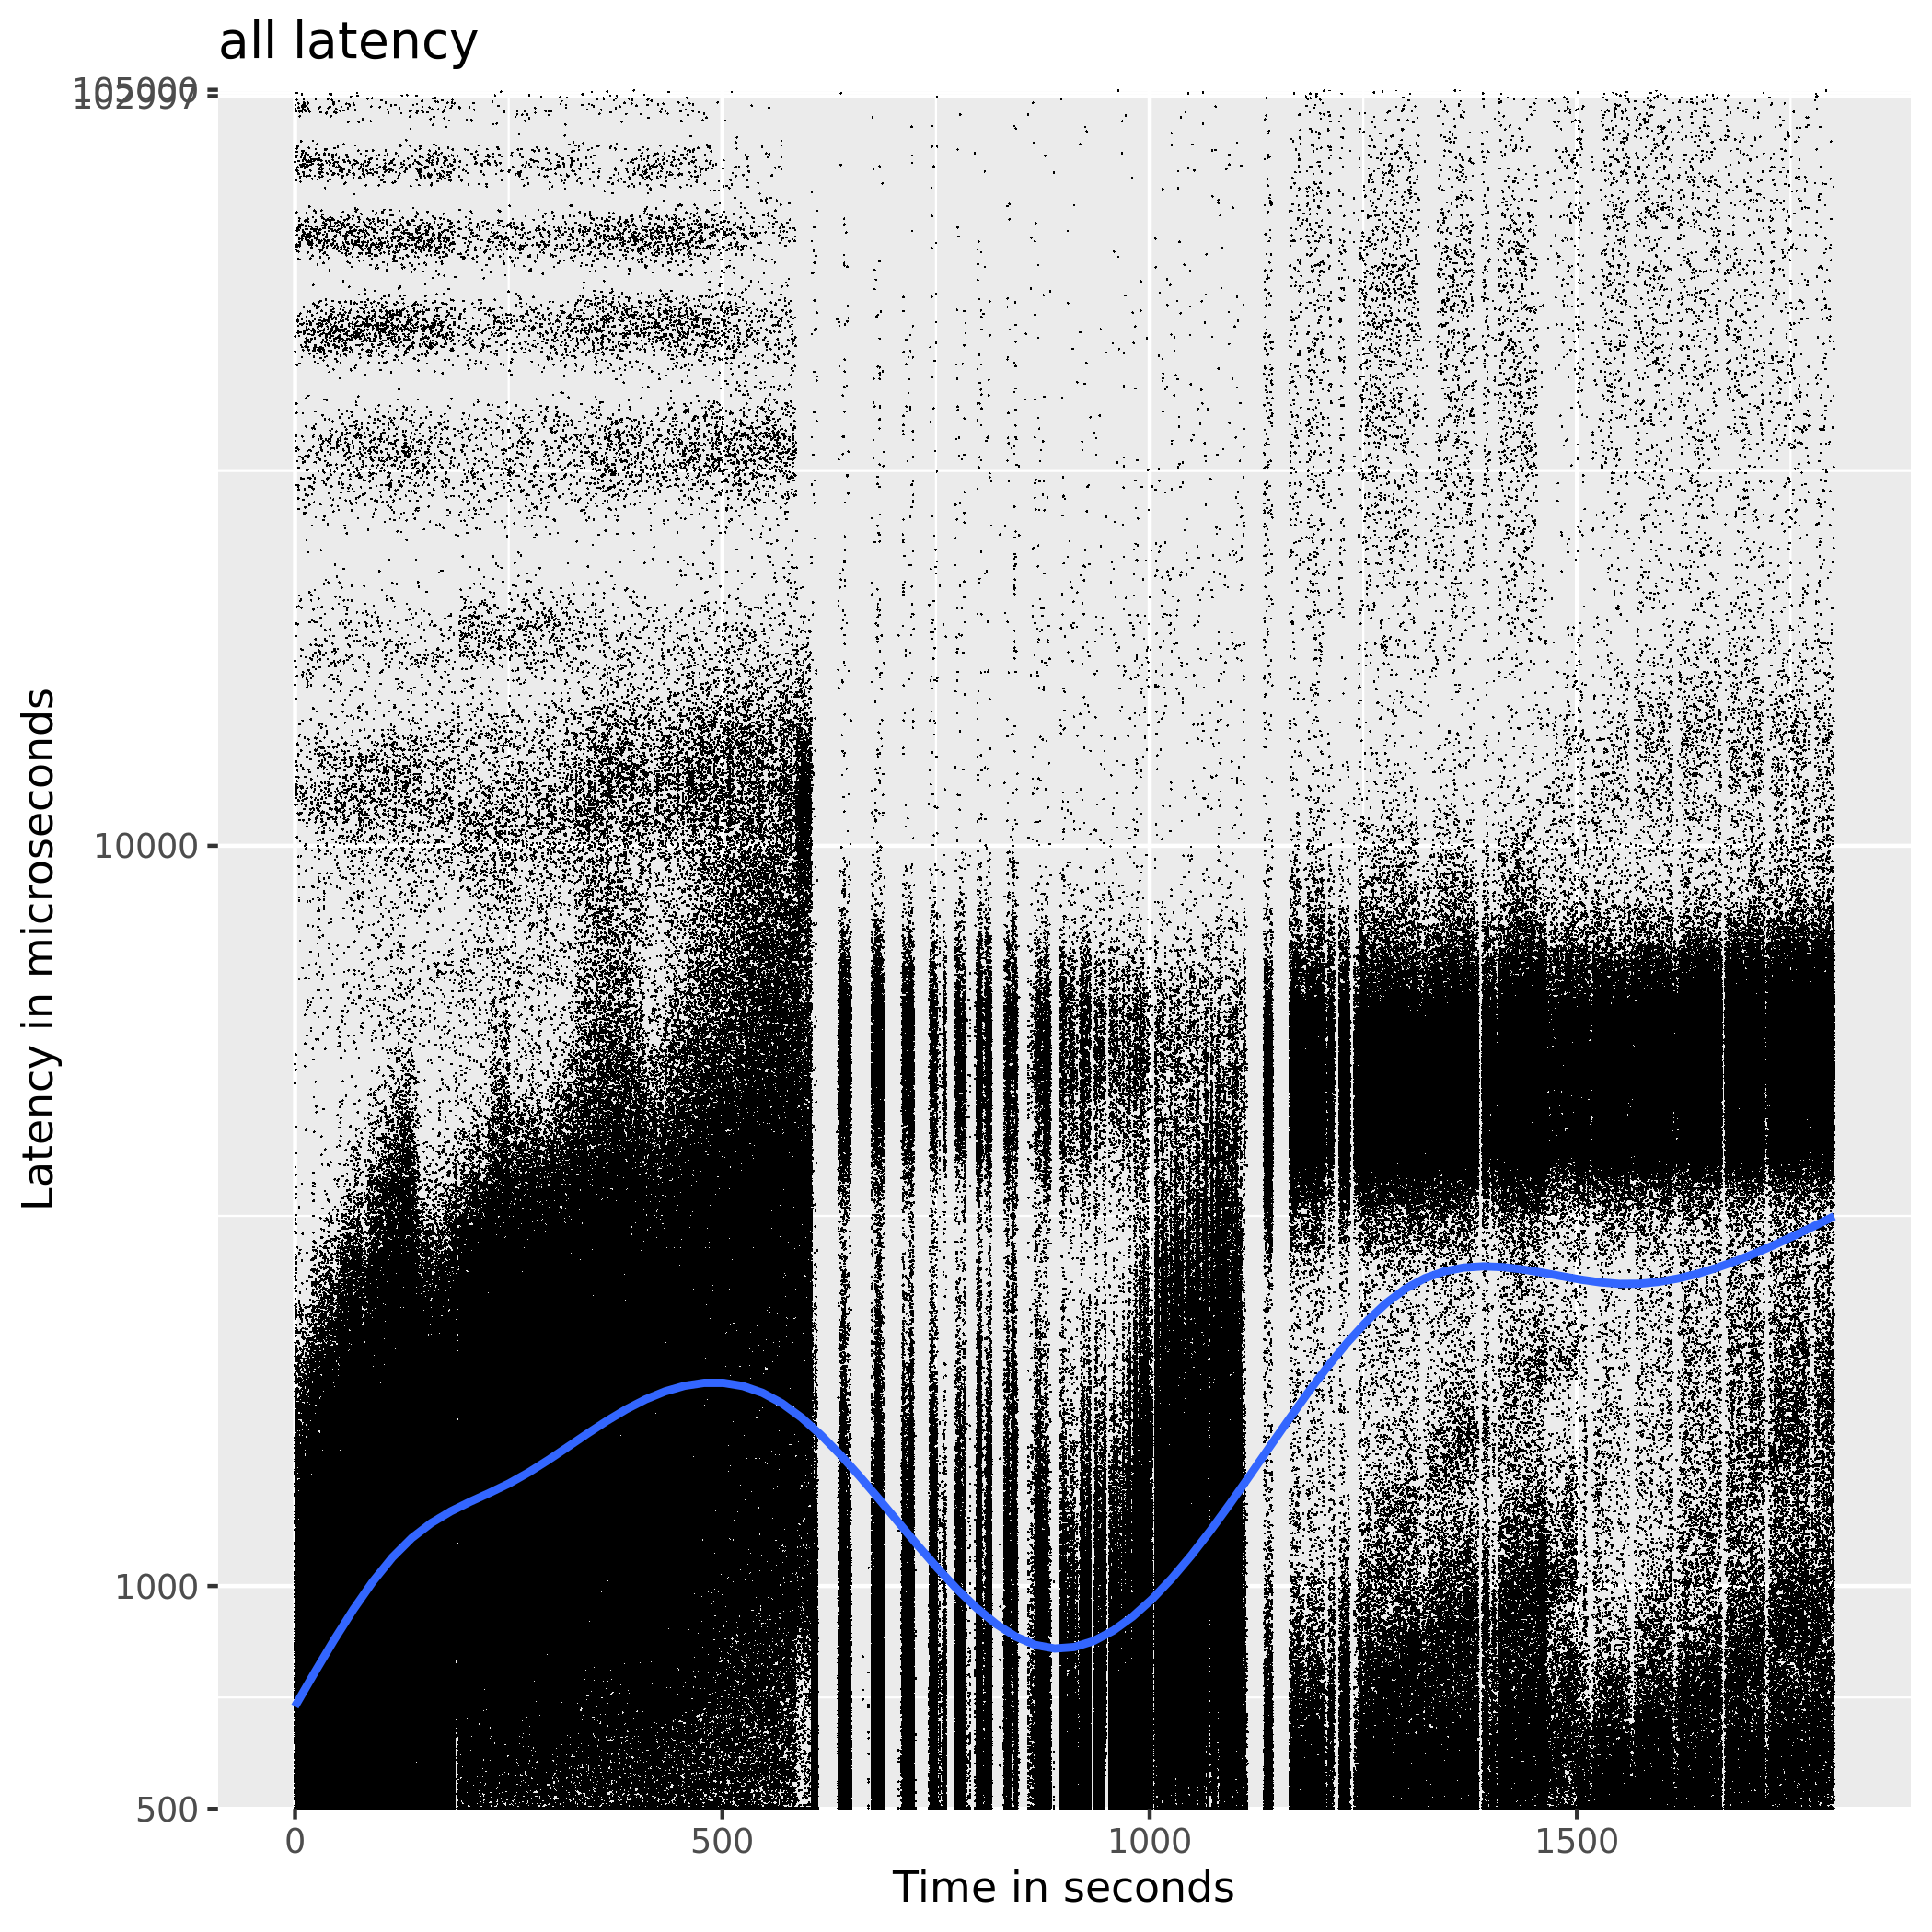
\includegraphics[width=0.8\textwidth]{RandomSlicing_Random_dynamic_write_heavy_latency}
	\caption[Latency for \ac{RS} with Write-Heavy Workload]{Latency for \ac{RS} with Write-Heavy Workload}
\end{subfigure}
\caption[Handoff Comparison]{Handoff Comparison. The hard edges in the latency plot can be used as an index to when the system is disrupted by handoff and repair operations.}
\label{fig:handoff_comparison}
\end{figure}
One can easily see that for the read-heavy workload the disruptions with \ac{RS} are way shorter than with Consistent Hashing.
However, with the write-heavy workload there are multiple small disruptions with \ac{RS} and less and shorter disruptions with Consistent Hashing.
Overall we can make no assertion on the hypothesis with the available data as the results are currently ambiguous and there is a need for more and different kinds of cluster changes to derive a conclusion.